


%###################################################################################################################################################
%###################################################################################################################################################
%######################################### FIRST CHAPTER ON PROBABILITY THEORY #####################################################################
%###################################################################################################################################################
%###################################################################################################################################################




%%%%%%%%%%%%%%%%%%%%%%%%%%%%%%%%%%%%%%%%%%%%%%%%%%%%%%%%%%%%%%%%%%%%%%%%%%%%%%%%%%%%%%%%%%%%%%%%%%%%%%%%%%%%%%%%%%%%%%%%%%%%%%%%%%%%%%%%%%%%%%%%%%%%%
%%%%%%%%%%%%%%%%%%%%%%%%%%%%%%%%%%%%%%%%%%%%%%%%%%%%%%%%%%%%%%%%%%%%%%%%%%%%%%%%%%%%%%%%%%%%%%%%%%%%%%%%%%%%%%%%%%%%%%%%%%%%%%%%%%%%%%%%%%%%%%%%%%%%%
%%%%%%%%%%%%%%%%%%%%%%%%%%%%%%%%%%%%%%%%%%%%%%%%%% FIRST LECTURE: EVENTS %%%%%%%%%%%%%%%%%%%%%%%%%%%%%%%%%%%%%%%%%%%%%%%%%%%%%%%%%%%%%%%%%%%%%%%%%%%%%
%%%%%%%%%%%%%%%%%%%%%%%%%%%%%%%%%%%%%%%%%%%%%%%%%%%%%%%%%%%%%%%%%%%%%%%%%%%%%%%%%%%%%%%%%%%%%%%%%%%%%%%%%%%%%%%%%%%%%%%%%%%%%%%%%%%%%%%%%%%%%%%%%%%%%


%%%%%%%%%%%%%%%%%%%%%%%%%%%%%%%%%%%%%%%%%%%%%%%%%%%%%%%%%%%%%%%%%%%%%%%%%%%%%%%%%%%%%%%%%%%%%%%%%%%%%%%%%%%%%%%%%%%%%%%%%%%%%%%%%%%%%%%%%%%%%%%%%%%%%%%%%%%%%%%%%%%%%%%%%%%%%%%%%%%%%%%%%%%%%%%%%%%%%%%%%%%%%%%%%%%%%%%%%%%
%%%%%%%%%%%%%%%%%%%%%%%%%%%%%%%%%%%%%%%%%%%%%%%%%%%%%%%%%%%%%%%%%%%%%%%%%%%%%%%%%%%%%%%%%%%%%%%%%%%%%%%%%%%%%%%%%%%%%%%%%%%%%%%%%%%%%%%%%%%%%%%%%%%%%%%%%%%%%%%%%%%%%%%%%%%%%%%%%%%%%%%%%%%%%%%%%%%%%%%%%%%%%%%%%%%%%%%%%%%
%%%%%%%%%%%%%%%%%%%%%%%%%%%%%%%%%%%%%%%%%%%%%% PROBABILITY THEORY %%%%%%%%%%%%%%%%%%%%%%%%%%%%%%%%%%%%%%%%%%%%%%%%%%%%%%%%%%%%%%%%%%%%%%%%%%%%>>>>>>>>>>>>%%%%%%%%%%%%%%%%%%%%%%%%%%%%%%%%%%%%%%%%%%%%%%%%%%%%%%%%%%%%%%%%
%%%%%%%%%%%%%%%%%%%%%%%%%%%%%%%%%%%%%%%%%%%%%%%%%%%%%%%%%%%%%%%%%%%%%%%%%%%%%%%%%%%%%%%%%%%%%%%%%%%%%%%%%%%%%%%%%%%%%%%%%%%%%%%%%%%%%%%%%%%%%%%%%%%%%%%%%%%%%%%%%%%%%%%%%%%%%%%%%%%%%%%%%%%%%%%%%%%%%%%%%%%%%%%%%%%%%%%%%%%
%%%%%%%%%%%%%%%%%%%%%%%%%%%%%%%%%%%%%%%%%%%%%%%%%%%%%%%%%%%%%%%%%%%%%%%%%%%%%%%%%%%%%%%%%%%%%%%%%%%%%%%%%%%%%%%%%%%%%%%%%%%%%%%%%%%%%%%%%%%%%%%%%%%%%%%%%%%%%%%%%%%%%%%%%%%%%%%%%%%%%%%%%%%%%%%%%%%%%%%%%%%%%%%%%%%%%%%%%%%

		

%%%%%%%%%%%%%%%%%%%%%%%%%%%%%%%%%%%%%%%%%%%%%%%%%%%%%%%%%%%%%%%%%%%%%%%%%%%%%%%%%%%%%%%%%%%%%%%%%%%%%%%%%%%%%%%%%%%%%%%%%%%%%%%%%%%%%%%%%%%%%%%%%%%%%%%%%%%%%%%%%%%%%%%%%%%%%%%%%%%%%%%%%%%%%%%%%%%%%
%%%%%%%%%%%%%%%%%%%%%%%%%%%%%%%%%%%%%%%%%%%%%%%%%%%%%%%%%%%%%%%%%%%%%%%%%%%%%%%%%%%%%%%%%%%%%%%%%%%%%%%%%%%%%%%%%%%%%%%%%%%%%%%%%%%%%%%%%%%%%%%%%%%%%%%%%%%%%%%%%%%%%%%%%%%%%%%%%%%%%%%%%%%%%%%%%%%%%
%%%%%%%%%%%%%%%%%%%%%%%%%%%%%%%%%%%%%%%%%%%%%%%%%%%%%%%%%%%%%%%%%%%%%%%%%%%%%%%%%%%%%%%%%%%%%%%%%%%%%%%%%%%%%%%%%%%%%%%%%%%%%%%%%%%%%%%%%%%%%%%%%%%%%%%%%%%%%%%%%%%%%%%%%%%%%%%%%%%%%%%%%%%%%%%%%%%%%
%%%%%%%%%%%%%%%%%%%%%%%%%%%%%%%%%%%%%%%%%%%%%%%% Measurable Space Category %%%%%%%%%%%%%%%%%%%%%%%%%%%%%%%%%%%%%%%%%%%%%%%%%%%%%%%%%%%%%%%%%%%%%%%%%%%%%%%%%%%%%%%%%%%%%%%%%%%%%%%%%%%%%%%%%%%%%%%%%%
%%%%%%%%%%%%%%%%%%%%%%%%%%%%%%%%%%%%%%%%%%%%%%%%%%%%%%%%%%%%%%%%%%%%%%%%%%%%%%%%%%%%%%%%%%%%%%%%%%%%%%%%%%%%%%%%%%%%%%%%%%%%%%%%%%%%%%%%%%%%%%%%%%%%%%%%%%%%%%%%%%%%%%%%%%%%%%%%%%%%%%%%%%%%%%%%%%%%%
%%%%%%%%%%%%%%%%%%%%%%%%%%%%%%%%%%%%%%%%%%%%%%%%%%%%%%%%%%%%%%%%%%%%%%%%%%%%%%%%%%%%%%%%%%%%%%%%%%%%%%%%%%%%%%%%%%%%%%%%%%%%%%%%%%%%%%%%%%%%%%%%%%%%%%%%%%%%%%%%%%%%%%%%%%%%%%%%%%%%%%%%%%%%%%%%%%%%%
%%%%%%%%%%%%%%%%%%%%%%%%%%%%%%%%%%%%%%%%%%%%%%%%%%%%%%%%%%%%%%%%%%%%%%%%%%%%%%%%%%%%%%%%%%%%%%%%%%%%%%%%%%%%%%%%%%%%%%%%%%%%%%%%%%%%%%%%%%%%%%%%%%%%%%%%%%%%%%%%%%%%%%%%%%%%%%%%%%%%%%%%%%%%%%%%%%%%%



	%%%%%%%%%%%%%%%%%%%%%%%%%%%%%%%%%%%%%%%%%%%%%%%%%%%%%%%%%%%%%%%%%%%%%%%%%%%%%%%%%%%%%%%%%%%%%%%%%%%%%%%%%%%%%%%%%%%%%%
	%%%%%%%%%%%%%%%%%%%%%%%%%%%%%%%%%%%%%%%%%%%%%%%%%%%%%%%%%%%%%%%%%%%%%%%%%%%%%%%%%%%%%%%%%%%%%%%%%%%%%%%%%%%%%%%%%%%%%%
	%%%%%%%%%%%%%%%%%%%%%%%%%%%% PROBABILITY SPACE CATEGORY %%%%%%%%%%%%%%%%%%%%%%%%%%%%%%%%%%%%%%%%%%%%%%%%%%
	%%%%%%%%%%%%%%%%%%%%%%%%%%%%%%%%%%%%%%%%%%%%%%%%%%%%%%%%I%%%%%%%%%%%%%%%%%%%%%%%%%%%%%%%%%%%%%%%%%%%%%%%%%%%%%%%%%%%%%%%
	%%%%%%%%%%%%%%%%%%%%%%%%%%%%%%%%%%%%%%%%%%%%%%%%%%%%%%%%%%%%%%%%%%%%%%%%%%%%%%%%%%%%%%%%%%%%%%%%%%%%%%%%%%%%%%%%%%%%%%

    %%%%%%%%%%%%%%%%%%%%%%%%%%%%%%%%%%%%%%%%%%%%%%%%%%%%%%%%%%%%%%%%%%%%%%%%%%%%%%%%%%%%%%%%%%%%%%%%%%%%%%%%%%%%%%%%%%%%%%%%%%%%%%%%%
    %%%%%%%%%%%%%%%%%%%%%%%%%%%%%%%%%%%%%%%%%%%%%%%%%%%%%%%%%%%%%%%%%%%%%%%%%%%%%%%%%%%%%%%%%%%%%%%%%%%%%%%%%%%%%%%%%%%%%%%%%%%%%%%%%
    %%%%%%%%%%%%%%%%%%%%%%%%%%%%%%%%%%% Section: Bernoulli Trials %%%%%%%%%%%%%%%%%%%%%%%%%%%%%%%%%%%%%%%%%%%%%%%%%%%%%%%%%%%%%%%%%%%
    %%%%%%%%%%%%%%%%%%%%%%%%%%%%%%%%%%%%%%%%%%%%%%%%%%%%%%%%%%%%%%%%%%%%%%%%%%%%%%%%%%%%%%%%%%%%%%%%%%%%%%%%%%%%%%%%%%%%%%%%%%%%%%%%%
    %%%%%%%%%%%%%%%%%%%%%%%%%%%%%%%%%%%%%%%%%%%%%%%%%%%%%%%%%%%%%%%%%%%%%%%%%%%%%%%%%%%%%%%%%%%%%%%%%%%%%%%%%%%%%%%%%%%%%%%%%%%%%%%%%

	

%%%%%%%%%%%%%%%%%%%%%%%%%%%%%%%%%%%%%%%%%%%%%%%%%%%%%%%%%%%%%%%%%%%%%%%%%%%%%%%%%%%%%%%%%%%%%%%%%%%%%%
    %%%%%%%%%%%%%%%%%%%%%%%%%%%%%%%%%%%%%%%%%%%%%%%%%%%%%%%%%%%%%%%%%%%%%%%%%%%%%%%%%%%%%%%%%%%%%%%%%%%%%%%%%%%%%%%%%%%%%%%%%%%%%%%%%
    %%%%%%%%%%%%%%%%%%%%%%%%%%%%%%%%%%%%%   SECTION: RANDOM VARIABLES %%%%%%%%%%%%%%%%%%%%%%%%%%%%%%%%%%%%%%%%%%%%%%%%%%%%%%%%%%%%%%%
    %%%%%%%%%%%%%%%%%%%%%%%%%%%%%%%%%%%%%%%%%%%%%%%%%%%%%%%%%%%%%%%%%%%%%%%%%%%%%%%%%%%%%%%%%%%%%%%%%%%%%%%%%%%%%%%%%%%%%%%%%%%%%%%%%
    %%%%%%%%%%%%%%%%%%%%%%%%%%%%%%%%%%%%%%%%%%%%%%%%%%%%%%%%%%%%%%%%%%%%%%%%%%%%%%%%%%%%%%%%%%%%%%%%%%%%%%%%%%%%%%%%%%%%%%%%%%%%%%%%%






\chapter{ Statistics}

	\section{Introduction: Data and Models}

\subsection{Data}
	\label{ss:data}
	
	One of scopes of statistics is to infer knowledge from data, which often comes in the form of many differnt instances of the same variables. Next we briefly introduce the kind of data we will deal with and the corresoponding types in R. First we differentiate between numerical variables and non-numerical variables. In between numerical variables we distinguish integer variables and real (continuous) variables. Integer variables usually come from counting procedures, e.g. the number of children, and real variables can be seen as those that require to fix a precision to truncate the decimal expansion, e.g. height in cm , which otherwise would go on indefinitely. 

\begin{knitrout}
\definecolor{shadecolor}{rgb}{0.969, 0.969, 0.969}\color{fgcolor}\begin{kframe}
\begin{alltt}
\hlkwd{typeof}\hldef{(}\hlnum{2}\hldef{)}
\end{alltt}
\begin{verbatim}
## [1] "double"
\end{verbatim}
\begin{alltt}
\hlkwd{class}\hldef{(}\hlnum{2}\hldef{)}
\end{alltt}
\begin{verbatim}
## [1] "numeric"
\end{verbatim}
\begin{alltt}
\hlkwd{typeof}\hldef{(}\hlnum{2L}\hldef{)}
\end{alltt}
\begin{verbatim}
## [1] "integer"
\end{verbatim}
\begin{alltt}
\hlkwd{class}\hldef{(}\hlnum{2L}\hldef{)}
\end{alltt}
\begin{verbatim}
## [1] "integer"
\end{verbatim}
\begin{alltt}
\hldef{sample_size} \hlkwb{<-} \hlnum{10000}
\hlcom{# We generate artificially a sample of integers}
\hldef{Age} \hlkwb{<-} \hlkwd{sample}\hldef{(}\hlnum{15}\hlopt{:}\hlnum{70}\hldef{, sample_size,} \hlkwc{replace} \hldef{= T )}
\hlkwd{typeof}\hldef{(Age)}
\end{alltt}
\begin{verbatim}
## [1] "integer"
\end{verbatim}
\begin{alltt}
\hlkwd{class}\hldef{(Age)}
\end{alltt}
\begin{verbatim}
## [1] "integer"
\end{verbatim}
\begin{alltt}
\hlcom{# We generate artificially a sample of continuous data }
\hldef{Income} \hlkwb{<-} \hlkwd{rexp}\hldef{( sample_size)}
\hlkwd{typeof}\hldef{(Income)}
\end{alltt}
\begin{verbatim}
## [1] "double"
\end{verbatim}
\begin{alltt}
\hlkwd{class}\hldef{(Income)}
\end{alltt}
\begin{verbatim}
## [1] "numeric"
\end{verbatim}
\end{kframe}
\end{knitrout}

Among non-numerical variables we are particularly interested in categorical variables, that is, in those variables that can assume only a finite number of values, e.g., the gender. The set of possible choices for the variable is denoted the set of levels, and this can be ordered or unordered. Ordered categorical variables are stored as an ordered factor in R and unorderd categorical variables in factors 
\begin{knitrout}
\definecolor{shadecolor}{rgb}{0.969, 0.969, 0.969}\color{fgcolor}\begin{kframe}
\begin{alltt}
\hldef{levels} \hlkwb{<-} \hlkwd{c}\hldef{(}\hlsng{'Formal'}\hldef{,} \hlsng{'Informal'}\hldef{)}
\hldef{Variant_char} \hlkwb{<-} \hlkwd{sample}\hldef{( levels, sample_size,} \hlkwc{replace} \hldef{= T,} \hlkwc{prob} \hldef{=} \hlkwd{c}\hldef{(}\hlnum{0.7}\hldef{,}\hlnum{0.3}\hldef{) )}
\hldef{Variant} \hlkwb{<-} \hlkwd{factor}\hldef{( Variant_char,} \hlkwc{levels} \hldef{= levels)}
\hlkwd{typeof}\hldef{(Variant)}
\end{alltt}
\begin{verbatim}
## [1] "integer"
\end{verbatim}
\begin{alltt}
\hlkwd{class}\hldef{(Variant)}
\end{alltt}
\begin{verbatim}
## [1] "factor"
\end{verbatim}
\begin{alltt}
\hlkwd{typeof}\hldef{(Variant_char)}
\end{alltt}
\begin{verbatim}
## [1] "character"
\end{verbatim}
\begin{alltt}
\hlkwd{class}\hldef{(Variant_char)}
\end{alltt}
\begin{verbatim}
## [1] "character"
\end{verbatim}
\begin{alltt}
\hldef{Education_levels} \hlkwb{<-} \hlkwd{c}\hldef{(}\hlsng{'Diploma'}\hldef{,} \hlsng{' Bachelor\textbackslash{}'s Degree'}\hldef{,} \hlsng{'Master\textbackslash{}'s Degree'}\hldef{,} \hlsng{'Ph.D.'}\hldef{)}
\hldef{Education_char} \hlkwb{<-} \hlkwd{sample}\hldef{(Education_levels, sample_size,} \hlkwc{replace} \hldef{= T )}
\hldef{Education} \hlkwb{<-} \hlkwd{factor}\hldef{( Education_char,} \hlkwc{levels} \hldef{= Education_levels,} \hlkwc{ordered} \hldef{= T )}
\hlkwd{typeof}\hldef{(Education)}
\end{alltt}
\begin{verbatim}
## [1] "integer"
\end{verbatim}
\begin{alltt}
\hlkwd{class}\hldef{(Education)}
\end{alltt}
\begin{verbatim}
## [1] "ordered" "factor"
\end{verbatim}
\end{kframe}
\end{knitrout}

	The  data in the previous chuck of code can be seen as the result of a linguistic experiment that consists in collecting data on the freqency with which one of the two variants, one formal and the onhter one informal, is used.  The data structure that we use to collect the data is the \emph{data fram}, whose ccolumns consist on different variables and whose rows are the different bservations of the same variable. Therefore, the  output of a linguistic experiment might look like 
\begin{knitrout}
\definecolor{shadecolor}{rgb}{0.969, 0.969, 0.969}\color{fgcolor}\begin{kframe}
\begin{alltt}
\hlkwd{library}\hldef{(uuid)}
\hldef{Informant_id} \hlkwb{=}\hlkwd{replicate}\hldef{(sample_size,} \hlkwd{UUIDgenerate}\hldef{( ))}
\hldef{Experiment_result} \hlkwb{<-}  \hlkwd{tibble}\hldef{(} \hlkwc{Informant_id} \hldef{= Informant_id,}  \hlkwc{Age} \hldef{= Age,} \hlkwc{Income} \hldef{= Income ,} \hlkwc{Education} \hldef{= Education, Variant  )}
\end{alltt}


{\ttfamily\noindent\bfseries\color{errorcolor}{\#\# Error in tibble(Informant\_id = Informant\_id, Age = Age, Income = Income, : non trovo la funzione "{}tibble"{}}}\begin{alltt}
\hlkwd{head}\hldef{(Experiment_result )}
\end{alltt}


{\ttfamily\noindent\bfseries\color{errorcolor}{\#\# Error in head(Experiment\_result): oggetto 'Experiment\_result' non trovato}}\end{kframe}
\end{knitrout}
The different columns represent the different variables  we are observing, while different rows correspond to different observations
	
% Here the problem is: How do I justify that the data that I am collecting are different instances of the same variable? 


\subsection{Models}
	\label{ss:models}
	Once the data into the tibble
\begin{knitrout}
\definecolor{shadecolor}{rgb}{0.969, 0.969, 0.969}\color{fgcolor}\begin{kframe}
\begin{alltt}
        \hlkwd{head}\hldef{(Experiment_result)}
\end{alltt}


{\ttfamily\noindent\bfseries\color{errorcolor}{\#\# Error in head(Experiment\_result): oggetto 'Experiment\_result' non trovato}}\end{kframe}
\end{knitrout}
	the crucial question becomes how to use it to infer knowledge about the variables. This is at its core a complicated question of epistemiology. Narrowing our scopes, recall form Subsection~\ref{ss:probability_motivation} that an empirical, probabilistic model for the data is the most we can hope for. Statistics uses the probability theory framework to see the observed data as an instance of all the different possible tibbles that we could have obtained, which constitutes the sample space
	\begin{equation}
		\Omega = \text{ The set of all possible tibbles}.
	\end{equation}
	The observed tibble is therefore an element of $\Omega$, and we can evaluate the probability, or degree of belief, of other possible tibbles. Denote by $\mathcal P= \{\mathbb P \,,\, \mathbb P \text{ is a probability over $\Omega$} \}$ the set of probability measures on $\Omega$. Rather counterintuitively, to make any use of the data we first need to make assumptions on it, as outlined in the following scheme
	\begin{itemize}
		\item We define our \emph{model}, that is, we make assumptions on the data $\Omega$. Formally, we fix a subset $ \mathcal Q \subset \mathcal P$, and we assume that the obtained tibble is extracted according to some distribution in $\mathcal Q$ . In other words, we restrict to consider not all the possible probabilities on $\Omega$, but only subset $\mathcal Q$ of them. Typically the subset $\mathcal Q$ is of the form $\mathcal Q = \{ \mathbb P_\theta, \theta \in \Theta\}$, where $\Theta$ is a set of indexes. In this case $\theta$ is said to be the parameter of the model, see Example~\ref{ex:Bernoulli_model} for an example where $\theta \equiv p$ and  $\Theta = [0,1]$. 
		\item 	Once we observe the data, we can try to guess which of the $\theta \in \Theta$ is more likely to have generated the data. That is, we \emph{infer} information on the parameter $\theta$. 
 \end{itemize}
	The above abstract framework requires an example

	\begin{example}[ Sampling]
		\label{ex:sampling_model}
		The model that it is used for sampling $k$ individuals from a population of $n$ individuals $\{a_1,\ldots a_n\}$ is the one of extractions with or without replacements. We consider for simplicity the case where replacement occurs, and the model consists in considering the people from the population you are extracting from as balls in an urn, see also Example~\ref{ex:balls_urn} and Example~\ref{ex:extractions_independence???}. The model consists on one single probability $\mathcal Q  = \{ \mathbb P\}$, the uniform probability on each one of the outcomes, collected in the sample space 
		\bel{}{
		\Omega = \{ x_1...x_n\}
		}
	We recall that this choice is due to the independence of the choice of each single person and on the fair (uniform) choice of each person,  see Example~\ref{e:}. However, this conditions are not so straightforward to achieve and statisticians organizing polls have to find ways to choose a person among the others in a way as uniform as possible. For instance, polls made by cell phone calls in the early 2000 would miss a good portion of the population. In Example~\ref{ex:sampling_feature}  that this sampling model when we restrict to look not at the individual but at a feature that culd be common between individuals, say the eye color, gives rise to different models.  
	\end{example}

	\begin{example}[Bernoulli trials]
		\label{ex:Bernoulli_model}
		Consider the vector \textit{ Variants } defined in Subsection~\ref{ss:data}, which consists in position $i$ the variant of the word used by the $i$-th informant. In non mathematical terms, the Bernoulli trials model for the vector \textit{ Variants} is the following. Each informant, independently one from another, tosses a coin of parameter $p \in [0,1]$ and uses the formal variant if the coin shows heads.
		To put this model in a more formal way, consider the vector $\underline X = (X_1, \ldots , X_n)$, where $n \in \mathbb N$ is the numbser of informants and $X_i$ indicates whether the formal variant has been used :   
	\begin{equation}
		\label{e:Bernoulli}
		X_i = \begin{cases}
			1 & \text{ if $i-$th informant used the Formal variant}\\
			0 & \text{otherwise},
			\end{cases}
		\end{equation}
for $i = 1, \ldots, n$. In the next chuck of code we define the vector $\underline X$ 
\begin{knitrout}
\definecolor{shadecolor}{rgb}{0.969, 0.969, 0.969}\color{fgcolor}\begin{kframe}
\begin{alltt}
\hldef{Variant_numeric} \hlkwb{=} \hlkwd{as.numeric}\hldef{( Variant} \hlopt{==} \hlsng{"Formal"}\hldef{)}
\hldef{Varian_numeric[}\hlnum{1}\hlopt{:}\hlnum{10}\hldef{]}
\end{alltt}


{\ttfamily\noindent\bfseries\color{errorcolor}{\#\# Error: oggetto 'Varian\_numeric' non trovato}}\end{kframe}
\end{knitrout}
The model consists in assuming that the real world data $\underline X$ has been extracted according to one of the distributions contained in the set $\mathcal Q = \{\mathbb P_p, p \in [0,1]\}$, where $\mathbb P_p$ is the Bernoulli trial measure defined in ~\ref{d:Bernoulli_trial}, which, for the sake of readibility, we recall next. 
Under this model, the probability of seeing the result $\underline x = (x_1, \ldots, x_n)$, where $x_{i} \in \{0,1\}$ for each $i =1,\ldots, n$,  is
\begin{equation}
	\label{e:Bernoulli1}
	\mathbb P_p( \underline X = \underline x ) =  p^{ x_1 + \ldots + x_n }(1-p )^{n - (x_1 + \ldots + x_n )}, 
\end{equation}
	Now, and only now, the question of which one of the $\mathbb P \in \mathcal Q $ is more likely to have generated the data is well posed. In the present case one is tempted to say that the data has been generated according to $\mathbb P_{\hat p}$, for $\hat p=$"The proportion of times the formal variant has been used". This intuitive claim, if $H_0$ is true, is a consequence of Theorem~\ref{t:LLN}, see Corollary~\ref{} 

\begin{knitrout}
\definecolor{shadecolor}{rgb}{0.969, 0.969, 0.969}\color{fgcolor}\begin{kframe}
\begin{alltt}
\hlkwd{mean}\hldef{(Variant_numeric)}
\end{alltt}
\begin{verbatim}
## [1] 0.6995
\end{verbatim}
\begin{alltt}
\hlcom{# This is a good guess for the coin parameter $p$. }
\end{alltt}
\end{kframe}
\end{knitrout}
Note that, in this case, the data has been actually generated using a Bernoulli trial measure of parameter $p = 0.7$ (compare it with the estimated one!) and, therefore, the model $\mathcal Q$ contains the actual distriution that has generated the data. 
	\end{example}

	 Despite being false in general, models are often useful. In some cases, as in the sampling case Example~\ref{ex:sampling_model} and the following, are even close to reality 
	 \begin{example}[Sampling 2]
		\label{ex:sampling_features}
	Assume we are sampling from a population, see Example~\ref{ex:sampling_model}, and that we are looking at some features rather than at the exact person extracted. If the feature is has only  two possibilities, 0 or 1, then the Bernoulli measure model, see Example~\ref{ex:Bernoulli_model} is a good model. As an example, consider we are performing a statistical analysis on the number of languages known by the Moscow population.  The whole population of Moscow is saved in the factor \textit{Moscow\_population}
\begin{knitrout}
\definecolor{shadecolor}{rgb}{0.969, 0.969, 0.969}\color{fgcolor}\begin{kframe}
\begin{alltt}
\hldef{levels} \hlkwb{<-} \hlkwd{c}\hldef{(}\hlsng{'Bilingual'}\hldef{,}\hlsng{'Not Bilingual'}\hldef{)}
\hldef{Moscow_population_char} \hlkwb{<-} \hlkwd{sample}\hldef{( levels,}  \hlkwc{size} \hldef{=}  \hlnum{1000000}\hldef{,} \hlkwc{replace} \hldef{= T,} \hlkwc{prob} \hldef{=} \hlkwd{c}\hldef{(}\hlnum{0.7}\hldef{,} \hlnum{0.3}\hldef{)  )}
\hldef{Moscow_population} \hlkwb{<-} \hlkwd{factor}\hldef{(Moscow_population_char,} \hlkwc{levels} \hldef{= levels)}
\hlcom{# This is the whole Moscow population  }
\end{alltt}
\end{kframe}
\end{knitrout}
	The whole population is unaccessible to us, and, in particular, we cannot see how many people are bilingual by the simple command
\begin{knitrout}
\definecolor{shadecolor}{rgb}{0.969, 0.969, 0.969}\color{fgcolor}\begin{kframe}
\begin{alltt}
\hldef{real_p} \hlkwb{<-} \hlkwd{mean}\hldef{( Moscow_population} \hlopt{==} \hlsng{'Bilingual'}\hldef{)}
\hldef{real_p}
\end{alltt}
\begin{verbatim}
## [1] 0.70049
\end{verbatim}
\end{kframe}
\end{knitrout}
	However we can take samples (where we allow to select the same person twice, even if this happens with small probability)
\begin{knitrout}
\definecolor{shadecolor}{rgb}{0.969, 0.969, 0.969}\color{fgcolor}\begin{kframe}
\begin{alltt}
\hldef{sample_size} \hlkwb{=} \hlnum{100}
\hldef{Sampled_results} \hlkwb{<-} \hlkwd{sample}\hldef{(Moscow_population, sample_size,} \hlkwc{replace} \hldef{= T)}
\hlkwd{head}\hldef{(Sampled_results)}
\end{alltt}
\begin{verbatim}
## [1] Not Bilingual Bilingual     Bilingual     Bilingual     Bilingual    
## [6] Bilingual    
## Levels: Bilingual Not Bilingual
\end{verbatim}
\end{kframe}
\end{knitrout}
		Each extraction is independent from another, and we extract a Bilingual citizen with probability \textit{ real\_p}, so that, denoting as usual a bilingual by 1 and a non bilingual by 0,  the corresponding vector of 0s and 1s follows a Bernoulli trial distribution $\mathbb P_{\text{p\_real}}$, see Definition~\ref{d:Bernoulli_trial}. The parameter $p_{\text{real}}$ is unknown to us, but we known that the distribution is one from the Bernoulli model  $\mathcal Q = \{ \mathbb P_p , p \in [0,1]\}$. 
	In more computational terms, by saying that the Bernoulli model is a good model for this experiment, we mean that the two  samples generated by the following code
\begin{knitrout}
\definecolor{shadecolor}{rgb}{0.969, 0.969, 0.969}\color{fgcolor}\begin{kframe}
\begin{alltt}
\hlcom{# The two commands }
\hldef{sample_size} \hlkwb{<-} \hlnum{100}
\hlkwd{sample}\hldef{(  Moscow_population,} \hlkwc{size} \hldef{= sample_size ,}  \hlkwc{replace} \hldef{= T)}
\end{alltt}
\begin{verbatim}
##   [1] Bilingual     Bilingual     Not Bilingual Bilingual     Bilingual    
##   [6] Bilingual     Not Bilingual Bilingual     Not Bilingual Bilingual    
##  [11] Not Bilingual Not Bilingual Bilingual     Not Bilingual Bilingual    
##  [16] Bilingual     Bilingual     Bilingual     Not Bilingual Not Bilingual
##  [21] Bilingual     Bilingual     Bilingual     Bilingual     Bilingual    
##  [26] Not Bilingual Not Bilingual Bilingual     Not Bilingual Bilingual    
##  [31] Bilingual     Bilingual     Bilingual     Bilingual     Not Bilingual
##  [36] Bilingual     Not Bilingual Bilingual     Not Bilingual Bilingual    
##  [41] Not Bilingual Bilingual     Bilingual     Bilingual     Bilingual    
##  [46] Bilingual     Bilingual     Bilingual     Not Bilingual Bilingual    
##  [51] Not Bilingual Bilingual     Bilingual     Bilingual     Bilingual    
##  [56] Bilingual     Bilingual     Bilingual     Bilingual     Bilingual    
##  [61] Bilingual     Bilingual     Bilingual     Bilingual     Bilingual    
##  [66] Bilingual     Not Bilingual Bilingual     Bilingual     Bilingual    
##  [71] Not Bilingual Bilingual     Not Bilingual Bilingual     Bilingual    
##  [76] Bilingual     Bilingual     Bilingual     Bilingual     Bilingual    
##  [81] Bilingual     Bilingual     Not Bilingual Bilingual     Bilingual    
##  [86] Bilingual     Bilingual     Bilingual     Not Bilingual Bilingual    
##  [91] Not Bilingual Not Bilingual Not Bilingual Bilingual     Not Bilingual
##  [96] Bilingual     Not Bilingual Bilingual     Bilingual     Bilingual    
## Levels: Bilingual Not Bilingual
\end{verbatim}
\begin{alltt}
\hlcom{# and}
\hlkwd{rbinom}\hldef{(} \hlkwc{n} \hldef{= sample_size,} \hlkwc{size} \hldef{=} \hlnum{1}\hldef{,} \hlkwc{prob} \hldef{=} \hlkwd{mean}\hldef{(}\hlkwd{as.numeric}\hldef{(Moscow_population} \hlopt{==} \hlsng{'Bilingual'}\hldef{)))}
\end{alltt}
\begin{verbatim}
##   [1] 0 1 0 1 0 0 1 1 1 1 1 1 1 0 1 1 1 0 1 0 1 1 1 1 1 1 1 1 1 0 1 1 1 1 1 1 1
##  [38] 0 1 1 1 1 0 1 1 0 1 1 1 1 0 0 1 0 0 0 1 0 0 0 0 0 1 0 1 1 1 1 0 1 0 0 0 1
##  [75] 0 0 0 0 1 0 1 0 1 0 1 1 1 1 0 1 1 1 1 1 1 1 0 1 1 1
\end{verbatim}
\begin{alltt}
\hlcom{# have the same distribuition. rbinom samples from an abstract population}
\end{alltt}
\end{kframe}
\end{knitrout}
	have the same distribution. Since the sampling model from the whole population in Example~\ref{e:sampling_model} is a good model for, then also, the 
	\end{example}

	Note the similarity between the two examples. In both cases we do not have access to the object we are sampling from, either if it is a real population or a generalized population (a distribution), but we can take samples from them. To summarise this section, what statistics does is to consider data as a sample from a set of possible distributions ($\mathcal Q$), and try to infer knowledge on teh distribution. 


	\begin{example}{Eugene Onegin 2 }
		\label{e:Eugene_Onegin2}
		In Example~\ref{ex:Eugene_Onegin1} we have introduced a sequence of 0s and 1s coming from drama texts, replacing the vowels therein by 0 and the consonants by 1, and we have saved it into the variable \textit{text\_01}. In the same Section~\ref{s:bernoulli_beyond} we also have introduced the following two models
		\begin{enumerate}
			\item \label{item:model_bernoulli} $H_0$  The sequence is extracted from a Bernoulli measure, that is, $\mathcal Q = \{ \mathbb P_p, p \in [0,1]\}$, see Definition~\ref{d:Bernoulli????}.
			\item \label{item:model_markov} $H_1$ The sequence is extracted from a Markov measure, that is, $\mathcal Q = \{ \mathbb P_{a,b}, a, b \in [0,1]\}$, see Definition~\ref{d:}
		\end{enumerate} 
		Once we have defined the models in plain terms, we can proceed estimating the parameters. As will be proved in Example~\ref{ex:} If $H_0$ is true a good estimate for $p$, denoted by  $\hat p$, is the proportion of 1s in the string, that is 
\begin{knitrout}
\definecolor{shadecolor}{rgb}{0.969, 0.969, 0.969}\color{fgcolor}\begin{kframe}
\begin{alltt}
\hldef{hat_p} \hlkwb{<-} \hlkwd{mean}\hldef{(text_01)}
\end{alltt}


{\ttfamily\noindent\bfseries\color{errorcolor}{\#\# Error in mean(text\_01): oggetto 'text\_01' non trovato}}\end{kframe}
\end{knitrout}
		Example~\ref{ex:} shows that, if $H_1$ is true, a good estimate for $a$ and $b$ are the proportion of jumps from 0 to 1 among all the jumps from 0 and the proportion of jumps from 1 to 0, among the total number of jumps from 1, respectively:  
\begin{knitrout}
\definecolor{shadecolor}{rgb}{0.969, 0.969, 0.969}\color{fgcolor}\begin{kframe}
\begin{alltt}
\hldef{n_01} \hlkwb{<-} \hlkwd{sum}\hldef{(from} \hlopt{==} \hlnum{0} \hlopt{&} \hldef{to} \hlopt{==} \hlnum{1}\hldef{)}
\end{alltt}


{\ttfamily\noindent\bfseries\color{errorcolor}{\#\# Error: oggetto 'from' non trovato}}\begin{alltt}
\hldef{n_00} \hlkwb{<-} \hlkwd{sum}\hldef{(from} \hlopt{==} \hlnum{0} \hlopt{&} \hldef{to} \hlopt{==} \hlnum{0}\hldef{)}
\end{alltt}


{\ttfamily\noindent\bfseries\color{errorcolor}{\#\# Error: oggetto 'from' non trovato}}\begin{alltt}
\hldef{n_10} \hlkwb{<-} \hlkwd{sum}\hldef{(from} \hlopt{==} \hlnum{1} \hlopt{&} \hldef{to} \hlopt{==} \hlnum{0}\hldef{)}
\end{alltt}


{\ttfamily\noindent\bfseries\color{errorcolor}{\#\# Error: oggetto 'from' non trovato}}\begin{alltt}
\hldef{n_11} \hlkwb{<-} \hlkwd{sum}\hldef{(from} \hlopt{==} \hlnum{1} \hlopt{&} \hldef{to} \hlopt{==} \hlnum{1}\hldef{)}
\end{alltt}


{\ttfamily\noindent\bfseries\color{errorcolor}{\#\# Error: oggetto 'from' non trovato}}\begin{alltt}
\hlcom{# Compute the proportions }
\hldef{a_hat} \hlkwb{<-} \hldef{n_01} \hlopt{/} \hldef{(n_00} \hlopt{+} \hldef{n_01)}  \hlcom{# P(1 | 0)}
\end{alltt}


{\ttfamily\noindent\bfseries\color{errorcolor}{\#\# Error: oggetto 'n\_01' non trovato}}\begin{alltt}
\hldef{b_hat} \hlkwb{<-} \hldef{n_10} \hlopt{/} \hldef{(n_10} \hlopt{+} \hldef{n_11)}  \hlcom{# P(0 | 1)}
\end{alltt}


{\ttfamily\noindent\bfseries\color{errorcolor}{\#\# Error: oggetto 'n\_10' non trovato}}\end{kframe}
\end{knitrout}

	We can also see the distriution of $Y$ under hteThe above two claims are, once more, a consequence of the Law of Large numbers~\ref{t:LLN}, see Corollary~\ref{c:}??
	Finally, notice that models are an oversimplification of reality, so that $\mathbb P(H_0) = \mathbb P(H_1)$. However, we are not interested in absolute probabilities but in relative probabilities, such as, for instance, the odds $\mathbb P(H_1)/\mathbb P(H_0)$, which tell you which of the two models you regard as more likely.  
	\end{example}

	

	\section{ Testing}
	
	Let $\Omega$ be the sample space of all the possible data we could have obtained in an experiment and assume we have modelled it according probabilistically by assigning probability measure $\mathbb P$, which also weights the probabilities of obtaining different data. However, the same data could be possibly have arisen from various other alternative models. We denote denote the initial probabilistic model $H_0$, and, byh theoretical considerations that are behind the system of study, we formulate alternative hypotheses $H_1$. Tests give you a decision rule and a frameork that allow to say that there is enough evidence to reject the null hypothesis and to say that the   and we wonder whether other alternative models might fit betteThe same data could have been obtained even if it were sampled from a different probability measure $\mathbb Q$. How to decide which model is more likely to be true? 
	\subsection{ A simple example: Deciding which distribution is more likely to have generated the data }
	\label{}
	Assume we are observing a random variable $X$, so that $\Omega$ is the set of all the possible values for it. To fix the ideas, think of $X$ as the logarithm of the reaction time to a linguistic stimulus. Imagine that reasearcher have long established the model

which constitutes the \emph{null hypothesis} $H_0$: $X$ distributes according to a normal of parameters $\mu = 1$ and $\sigma = 2$.  Your own research suggests that $X$ would rather follow the distribution

Assume that we obser	
		\begin{example}[T]
			
		\end{example}

	\subsection{ Ideas and Terminology}
	Every statistical test follows the same intuitive framework, which we introduce by means of a simple example. A magician claims to have magical abilities and we decide to test whether it is true or not by the following \emph{experiment}. I will toss a fair coin $n$ times, each time making the coin hit the table and then falling to the floor (in this way the tosses are independent). In the meantime, the magician will try to use his abilities to make the coin show more often heads than tails.
	The hypotheses we want to test are two, the \emph{null hypothesis} $H_0$, which is the conservative one, which states that he is not a magician and \emph{alternative} hypothesis $H_1$, that tells us that he is a magician. This, however, is unprecise, since the hypotheses are precise statements on the model, that is, the probability, with which the data obtained in the experiment distribute: 
	\begin{itemize}
		\item  $H_0$ The coin tosses follow a Bernoulli trial measure of parameter $p = 1/2$ (independent tosses of a fair coin)
		\item $H_1$: $p>1/2$
	\end{itemize}
	Would the result $HHH$ be sufficient to \emph{reject $H_0$ } in favour of $H_1$? No, the result could be due to chance, that is, it is an "unlikely" result of $H_0$ even if it would be less unlikely under $H_1$. 
	On the other extremum, $HHHHHHHHHHHHHHHHHTTTHHHHHHHHHTHHHHH$ would suffice. The reason is that the result seems so unlikely under $H_0$ that maybe $H_0$ is not true. A test is a sort of statistical proof by contraddiction: we cannot say that the results are impossible if $H_0$ is true, but we can say that they are very unlikely. \\
	However we must make precise what unlikely means, since every string has the same probability. We define the \emph{statistic} of the number of heads as 
	\begin{equation}
		\label{e:heads_numbers}
		H(\underline X) = X_1 + \ldots + X_n
	\end{equation}
	where $X_i$ is $1$ if the $i$-th toss gave heads and $0$ otherwise and $\underline X= (X_1, \ldots, X_n)$ denotes the vector of the coin tosses. $H$ behaves differently whether $H_0$ or $H_1$ holds, and in the second case tends to be bigger. We recognize that in the long sequence the statistic $H(\underline X)$ attains a value that is not typical if $H_0$ were true.\\
	Having fixed a statistic and a notion of extremality ( extremal results are the ones where $H>> n/2$ ), the decision rule is therefore to fix a $h_{\text{crit}}$ and say that if $H(\underline X ) > h_{\text{crit}}$ we reject $H_0$ in favour of $H_1$. The scheme is given in Figure~\ref{f:type_errors} and the test is defined once we fix $h_{\text{crit}}$. \\
	\begin{figure}[h]
			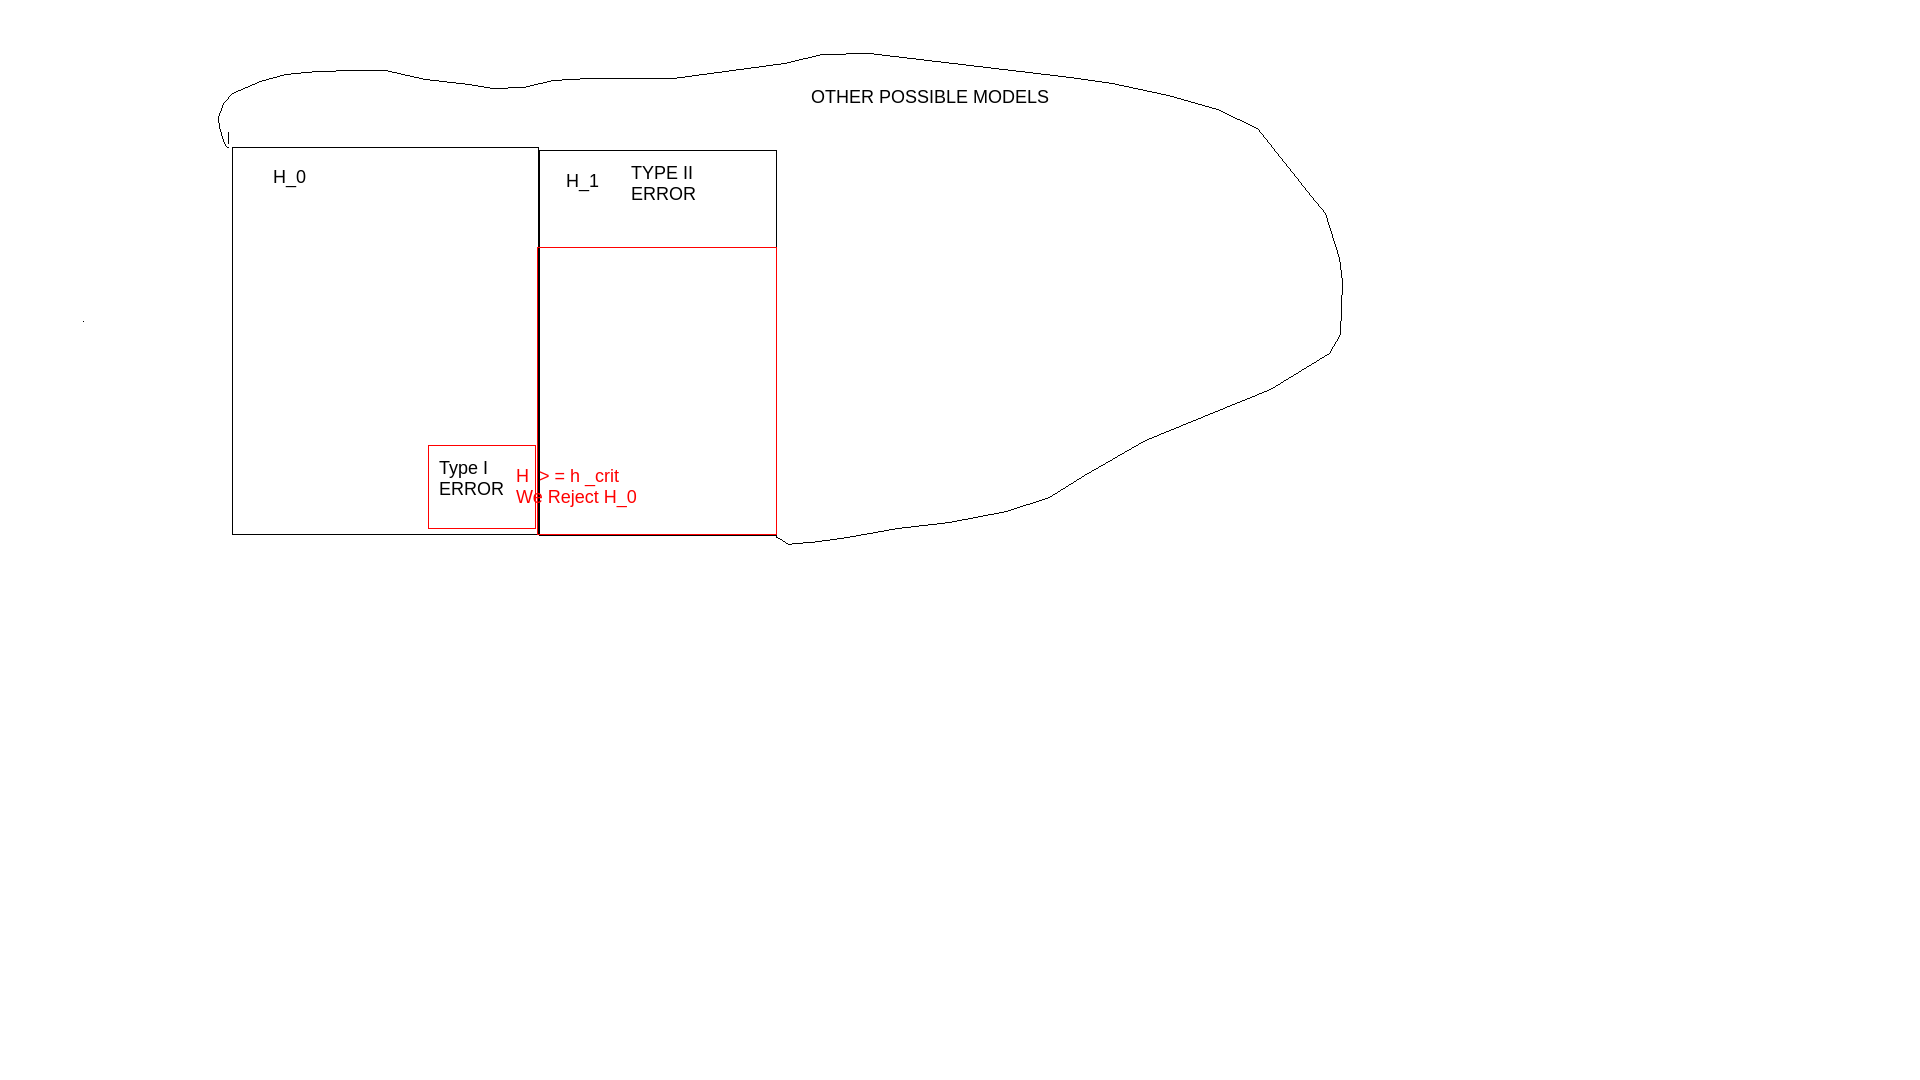
\includegraphics[width=14cm]{test.png}
		\label{f:type_errors}
	\end{figure}
This decistion rule, however, cannot lead out ( by the statistical nature of the two hypotheses) the possibility of two kind of errors, see Figure~\ref{f:type_errors}: type I error, where we reject $H_0$ in favour of $H_1$ while $H_0$ is true, and type II error, where we keep $H_0$, while $H_1$ is true.
That is, if $H > h_{\text{crit}}$,  while $H_0$ is true, we say that $H$ is extremal due to randomness and we are committing a type I error. Otherwise, if $H < h_{\text{crit}}$ and $H_1$ holds, we fail to see a real effect and we speak about type II error. 
	Since it is arguabilty more dangerous to arrogate to a normal person the condition of magicianthan not recognizing that a person is a magician, we would like to have a control on the type I error. We therefore fix a \emph{significance level} $\alpha$, usually $\alpha = 0.05$, and we impose that if $H_0$ holds, we accept that we can make an error with probability $\alpha$: 
	\begin{equation}
		\label{e:value}
		\mathbb P( \text{"$H_0$ rejected}|H_0)  = \mathbb P( H \geq h_{\text{crit}} | H_0) = \alpha
	\end{equation}
	In graphical terms, we choose $h_{\text{crit }}$ in such a way that the area in red in the $H_0$ part, see Figure~\ref{e:type_errors}, that is $H_0 \cap \{ H > h_{\text{crit}}\}$ is a $\alpha$ of the total area of $H_0$. The relation \eqref{e:value} defines $h_{\text{crit}}  = h_{\text{crit}}(\alpha)$, so that the decision rule is defined provided once we fix a significance level (see the end of this Subsection for the solvability the relation \eqref{e:value} between $\alpha$ and $h_{\text{crit}}$.)  
	We now fix $\alpha = 0.05$ and try to guess $h_{\text{crit}}$ for $n = 8$ tosses.  In the next subsection, we will see how the $h_{\text{crit}}$ is found with simple R commands 
\begin{knitrout}
\definecolor{shadecolor}{rgb}{0.969, 0.969, 0.969}\color{fgcolor}\begin{kframe}
\begin{alltt}
\hlcom{# We know that if H_0  is true }
\hlcom{# H distributes as a binomial }
\hlcom{# of parameters n = 10, p = 1/2}
\hlcom{# We now plot on the P( H = i | H_0) vs i }
\hldef{alpha} \hlkwb{=} \hlnum{0.05}
\hldef{n} \hlkwb{=} \hlnum{10}
\hldef{h_guess} \hlkwb{<-} \hlnum{10} \hlcom{# We observe 8 heads}
\hlkwd{ggplot}\hldef{(}\hlkwc{data} \hldef{=} \hlkwd{tibble}\hldef{(}\hlkwc{x} \hldef{=} \hlnum{0}\hlopt{:}\hldef{n,} \hlkwc{y} \hldef{=} \hlkwd{dbinom}\hldef{(}\hlnum{0}\hlopt{:}\hldef{n,} \hlkwc{size} \hldef{= n,}  \hlkwc{prob} \hldef{=} \hlnum{1}\hlopt{/}\hlnum{2}\hldef{)))} \hlopt{+}
        \hlkwd{geom_point}\hldef{(}\hlkwd{aes}\hldef{(x,y))} \hlopt{+}
        \hlkwd{geom_vline}\hldef{(}\hlkwc{xintercept} \hldef{= h_guess,} \hlkwc{col} \hldef{=} \hlsng{'red'}\hldef{)}
\end{alltt}


{\ttfamily\noindent\bfseries\color{errorcolor}{\#\# Error in ggplot(data = tibble(x = 0:n, y = dbinom(0:n, size = n, prob = 1/2))): non trovo la funzione "{}ggplot"{}}}\begin{alltt}
\hlcom{# P( H => 8 | H _0 ) = P( H = 10 | H_0) + P(H = 9 | H_0) + P( H = 8 | H_0)}
\hlcom{# We have to sum the height of the points on the right hand side of the }
\hlcom{# vertical line}
\hlkwd{sum}\hldef{(} \hlkwd{dbinom}\hldef{(h_guess}\hlopt{:}\hldef{n, n,} \hlkwc{prob} \hldef{=} \hlnum{1}\hlopt{/}\hlnum{2}\hldef{))}
\end{alltt}
\begin{verbatim}
## [1] 0.0009765625
\end{verbatim}
\begin{alltt}
\hlcom{# pbinom sums the heights on teh left hand side. Therefore }
\hlnum{1}\hlopt{-}\hlkwd{pbinom}\hldef{( h_guess} \hlopt{-}\hlnum{1} \hldef{,} \hlkwc{size} \hldef{= n,} \hlkwc{prob} \hldef{=} \hlnum{1}\hlopt{/}\hlnum{2}\hldef{)}
\end{alltt}
\begin{verbatim}
## [1] 0.0009765625
\end{verbatim}
\begin{alltt}
\hlcom{# The result is smaller than alpha = 0.05, let's try  }
\hlcom{# to repeat the code with a smaller guess. }
\hldef{h_guess} \hlkwb{<-} \hlnum{9}
\hlnum{1}\hlopt{-} \hlkwd{pbinom}\hldef{( (h_guess}\hlopt{-}\hlnum{1}\hldef{),}\hlkwc{size} \hldef{= n,} \hlkwc{prob} \hldef{=} \hlnum{1}\hlopt{/}\hlnum{2}\hldef{)}
\end{alltt}
\begin{verbatim}
## [1] 0.01074219
\end{verbatim}
\begin{alltt}
\hlcom{# It is still smaller than 0.05. Let's try to see whether }
\hlcom{# the type I error probability that we make if h_crit = 8 is }
\hlcom{# still smaller than alpha}
\hldef{h_guess} \hlkwb{<-} \hlnum{8}
\hlnum{1}\hlopt{-} \hlkwd{pbinom}\hldef{( (h_guess}\hlopt{-}\hlnum{1}\hldef{),}\hlkwc{size} \hldef{= n,} \hlkwc{prob} \hldef{=} \hlnum{1}\hlopt{/}\hlnum{2}\hldef{)}
\end{alltt}
\begin{verbatim}
## [1] 0.0546875
\end{verbatim}
\begin{alltt}
\hlcom{# No, therefore h_crit = 9 }


\hldef{h_guess} \hlkwb{<-} \hlnum{9} \hlcom{# We observe 8 heads}
\hlkwd{ggplot}\hldef{(}\hlkwc{data} \hldef{=} \hlkwd{tibble}\hldef{(}\hlkwc{x} \hldef{=} \hlnum{0}\hlopt{:}\hldef{n,} \hlkwc{y} \hldef{=} \hlkwd{dbinom}\hldef{(}\hlnum{0}\hlopt{:}\hldef{n,} \hlkwc{size} \hldef{= n,}  \hlkwc{prob} \hldef{=} \hlnum{1}\hlopt{/}\hlnum{2}\hldef{)))} \hlopt{+}
        \hlkwd{geom_point}\hldef{(}\hlkwd{aes}\hldef{(x,y))} \hlopt{+}
        \hlkwd{geom_vline}\hldef{(}\hlkwc{xintercept} \hldef{= h_guess,} \hlkwc{col} \hldef{=} \hlsng{'red'}\hldef{)}
\end{alltt}


{\ttfamily\noindent\bfseries\color{errorcolor}{\#\# Error in ggplot(data = tibble(x = 0:n, y = dbinom(0:n, size = n, prob = 1/2))): non trovo la funzione "{}ggplot"{}}}\begin{alltt}
\hlcom{# The quantile function finds immediatly the critical value}
\hlkwd{qbinom}\hldef{(}\hlnum{1}\hlopt{-}\hldef{alpha,} \hlkwc{size} \hldef{= n,} \hlkwc{prob} \hldef{=} \hlnum{1}\hlopt{/}\hlnum{2} \hldef{)}
\end{alltt}
\begin{verbatim}
## [1] 8
\end{verbatim}
\end{kframe}
\end{knitrout}
You might have noted that \eqref{e:value} is not always solvable for discrete distributions, since usually there is no $h$ such that $\mathbb P(H > h |H_0) = \alpha$ precisely. This technicality is overcomed by choosing $h_{\text{crit}}$ to be the leftmost element for which $\mathbb P( H \geq h_{\text{crit}} | H_0) \leq\alpha$. 

	We finish this section by introducing the concept of p-value. The p-value of an observed value $h_\text{obs}$ is the probability of obtaining a more extremal result, \textbf{provided $H_0$ holds}. Since in this case more extremal means greater, the $p-value$ of $h$ is 
	\begin{equation}
		\label{e:p-value}
		\mathbb P( H > h | H_0)
	\end{equation}
\begin{knitrout}
\definecolor{shadecolor}{rgb}{0.969, 0.969, 0.969}\color{fgcolor}\begin{kframe}
\begin{alltt}
\hlcom{# The p-value of h_obs = 7}
\hldef{h_obs} \hlkwb{<-} \hlnum{7}
\hlkwd{sum}\hldef{(} \hlkwd{dbinom}\hldef{(h_obs}\hlopt{:}\hldef{n,} \hlkwc{size} \hldef{= n,} \hlkwc{prob} \hldef{=} \hlnum{1}\hlopt{/}\hlnum{2}\hldef{))}
\end{alltt}
\begin{verbatim}
## [1] 0.171875
\end{verbatim}
\begin{alltt}
\hlnum{1}\hlopt{-} \hlkwd{pbinom}\hldef{(h_obs} \hlopt{-} \hlnum{1}\hldef{,} \hlkwc{size} \hldef{= n,} \hlkwc{prob} \hldef{=} \hlnum{1}\hlopt{/}\hlnum{2}\hldef{)}
\end{alltt}
\begin{verbatim}
## [1] 0.171875
\end{verbatim}
\end{kframe}
\end{knitrout}
	It is easy to prove that $h > h_{\text{crit}}$ if and only if the p-value associated to $h$ is smaller than $\alpha$. Therefore the decision rule can be equivalently restated as: " We reject $H_0$ in favour of $H_1$ if and only if the p-value of the statistic is smaller than $\alpha$".  
	
	\subsection{Binomial Test}

	The binomial test is used for data collected from a categorical data with two levels, where the observations are independent and one from  another and equally distributed. We come back to the Linguistic experiment where the informants will usa a word which has two variants, a formal one and an informal one.  
and we define $X_1, \ldots, X_n $ by setting $X_i = 1 $ if the $i$-th infomant said the Formal variant , 0 otherwise. 
	A research suggested that across Russia, a good model for the $X_i$ is the follwing: each person tosses, independently from the others, a coin of parameter $p$ and say the Formal variant if the coin gives heads. They estimated $p = 0.6$. 
	However, backed by some considerations, you think that for Moscow $p> 0.6$ and you collect some data to verify this

Therefore you reproduce the experiment with informants from the Moscow region. The data is collected in the column \textit{Variant} of the tibble \textit{ Experiment\_result}
\begin{knitrout}
\definecolor{shadecolor}{rgb}{0.969, 0.969, 0.969}\color{fgcolor}\begin{kframe}
\begin{alltt}
\hlkwd{head}\hldef{(Experiment_result}\hlopt{$}\hldef{Variant)}
\end{alltt}


{\ttfamily\noindent\bfseries\color{errorcolor}{\#\# Error in head(Experiment\_result\$Variant): oggetto 'Experiment\_result' non trovato}}\end{kframe}
\end{knitrout}
	The \emph{ null hypothesis}, which corresponds to the current model accepted, is 
	\begin{itemize}
		\item 	$H_0$: $X_1, \ldots, X_n $ are  Bernoulli trials of parameter $p = 0.6$
		\item $H_1$: $p>0.6$.
	\end{itemize}
	The statistic to use is the number of formal variants used. 
	\begin{ExerciseList}
		\Exercise Take a look at the previous chuncks of code. Is $H_0$ true? Is $H_1$ true?  The test tries to give a rule to decide this question in the real cases, where we cannot look at the "code" that has generated the data. 
	\end{ExerciseList}
		Let's check the $h_{\text{crit}}$  for this test and compute the p-value for teh observed $H$. The quantile function is the inverse of $h \to \mathbb P( H \leq h | H_0)$, and to find $h_{\text{crit}}(\alpha)$ we need to use it. 
\begin{knitrout}
\definecolor{shadecolor}{rgb}{0.969, 0.969, 0.969}\color{fgcolor}\begin{kframe}
\begin{alltt}
\hldef{sample_size} \hlkwb{<-} \hlkwd{length}\hldef{(Experiment_result}\hlopt{$}\hldef{Variant )}
\end{alltt}


{\ttfamily\noindent\bfseries\color{errorcolor}{\#\# Error: oggetto 'Experiment\_result' non trovato}}\begin{alltt}
\hldef{alpha} \hlkwb{=} \hlnum{0.05}
\hldef{p} \hlkwb{<-} \hlnum{0.6}
\hldef{h_obs} \hlkwb{<-} \hlkwd{sum}\hldef{(Experiment_result}\hlopt{$}\hldef{Variant} \hlopt{==}\hlsng{'Formal'}\hldef{)}
\end{alltt}


{\ttfamily\noindent\bfseries\color{errorcolor}{\#\# Error: oggetto 'Experiment\_result' non trovato}}\begin{alltt}
\hldef{h_crit} \hlkwb{<-} \hlkwd{qbinom}\hldef{(} \hlnum{1}\hlopt{-} \hldef{alpha,}\hlkwc{size} \hldef{= sample_size,} \hlkwc{prob} \hldef{= p )}
\hlkwd{ggplot}\hldef{(} \hlkwc{data} \hldef{=} \hlkwd{tibble}\hldef{(}\hlkwc{x} \hldef{=} \hlnum{0}\hlopt{:}\hldef{sample_size ,} \hlkwc{y} \hldef{=} \hlkwd{dbinom}\hldef{(}\hlnum{0}\hlopt{:}\hldef{sample_size,} \hlkwc{size} \hldef{= sample_size,} \hlkwc{prob} \hldef{= p )))} \hlopt{+}
 \hlkwd{geom_point}\hldef{(}\hlkwd{aes}\hldef{(x, y ))} \hlopt{+}
 \hlkwd{geom_vline}\hldef{(}\hlkwc{xintercept} \hldef{= h_obs,} \hlkwc{col} \hldef{=} \hlsng{'red'}\hldef{)} \hlopt{+}
 \hlkwd{geom_vline}\hldef{(}\hlkwc{xintercept} \hldef{= h_crit,} \hlkwc{col} \hldef{=} \hlsng{'blue'} \hldef{)}
\end{alltt}


{\ttfamily\noindent\bfseries\color{errorcolor}{\#\# Error in ggplot(data = tibble(x = 0:sample\_size, y = dbinom(0:sample\_size, : non trovo la funzione "{}ggplot"{}}}\begin{alltt}
 \hlcom{# To compute the mass on the right side of teh curve we use }
\end{alltt}
\end{kframe}
\end{knitrout}
We repeat once more that the test can be seen as a way to decide wether $h_\text{obs}$ has been sampled from the distribution shown in the above graph or by some other. R has a command to perform the binomial test.
\begin{knitrout}
\definecolor{shadecolor}{rgb}{0.969, 0.969, 0.969}\color{fgcolor}\begin{kframe}
\begin{alltt}
\hldef{n_formal} \hlkwb{<-} \hlkwd{sum}\hldef{( Experiment_result}\hlopt{$}\hldef{Variant} \hlopt{==} \hlsng{'Formal'}\hldef{)}
\end{alltt}


{\ttfamily\noindent\bfseries\color{errorcolor}{\#\# Error: oggetto 'Experiment\_result' non trovato}}\begin{alltt}
\hldef{n_total} \hlkwb{<-} \hlkwd{length}\hldef{(Experiment_result}\hlopt{$}\hldef{Variant)}
\end{alltt}


{\ttfamily\noindent\bfseries\color{errorcolor}{\#\# Error: oggetto 'Experiment\_result' non trovato}}\begin{alltt}
\hlkwd{binom.test}\hldef{( n_formal, n_total ,} \hlkwc{alternative} \hldef{=} \hlsng{'greater'}\hldef{)}
\end{alltt}


{\ttfamily\noindent\bfseries\color{errorcolor}{\#\# Error in binom.test(n\_formal, n\_total, alternative = "{}greater"{}): oggetto 'n\_formal' non trovato}}\end{kframe}
\end{knitrout}

	\begin{example}[Eugene Onegin 3: Binomial Test]
		\label{ex:Eugene_Onegin3}
		We now come back to the Eugene Onegin case, see Example~\ref{ex:Eugene_Onegin1} and \ref{ex:Eugene_Onegin2}, where we created a sequence of 0s and 1s, stored in the vector \textit{text\_01 }, in which the charcters of the texts of the german drama corpus where replaced by 1, if the character is was a consonant, 0, if it was a vowel, and simply omitted if it was any other character. In Example~\ref{ex:Eugene_Onegin2} we introduced two models for the sequence, $H_0$, in which the digits are i.i.d. with some parameter $p$, and we have estimated the parameter $p$ by the proportion of 1s in the sample, 
\begin{knitrout}
\definecolor{shadecolor}{rgb}{0.969, 0.969, 0.969}\color{fgcolor}\begin{kframe}
\begin{alltt}
\hlkwd{mean}\hldef{(text_01)}
\end{alltt}


{\ttfamily\noindent\bfseries\color{errorcolor}{\#\# Error in mean(text\_01): oggetto 'text\_01' non trovato}}\end{kframe}
\end{knitrout}
	and the reason will be clear in after having introduced the Law of Large Numbers~\ref{t:LLN} and its application in Example~\ref{}. We now want to see that by looking at the jumps from 0 to 1 and from 1 to 0 that this model is wrong. 


	Denote the string in \textit{text\_01} by $x_1x_2\ldots x_N$, for some $N \in\ mathbb N $, and let $n_0$ denote the number of zeros and  
	At an intuitive level, we think that the digits are not independent, since it is difficult to pronounce a word without consonants, and we will
	Now we will perform a binomial test on a different sequence related to the jumps from 0. Assume that $n_0$ is the number of 0s in the squence and denote by $\alpha(i)$ the position of the $i$-th zero, for $i = 1, \ldots, n_0$. The define the sequence $Y_i$, for $i = 1, \ldots, n_0$, indicating if from the 0 at the $\alpha(i)$-th position the sequence jumps to a 1, namely 
	\begin{equation}
	\label{e:interface}
		Y_i = \begin{cases}
			1 & \text{if $ X_{\alpha(i) + 1 } = 1$ }\\
			0 & \text{otherwise}
		\end{cases}
	\end{equation}
	Let's give an example for concreteness. For the sequence $100101$, $n_0= 3 $ and $\alpha(1) =2$, $\alpha(2) = 3$ and $\alpha(3) = 5$. $Y_1 = 0 $ since its first 0 is followed by a 0, $Y_2 = Y_3 =1$s since the last two zeros are followed by a 1. Graphically    
\[
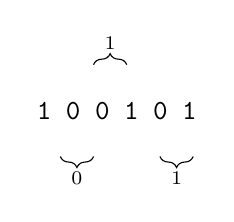
\begin{tikzpicture}[baseline=(seq.base)]
  \node (seq) at (0,0) {\texttt{1 0 0 1 0 1}};
  % Underbrace: 0 → 0
  \draw[decorate,decoration={brace,mirror,amplitude=4pt}]
    ([xshift=1.2em,yshift=-1.0em]seq.south west) -- 
    ([xshift=2.4em,yshift=-1.0em]seq.south west)
    node[midway,below=2pt]{\scriptsize 0};

  % Overbrace: 0 → 1
  \draw[decorate,decoration={brace,amplitude=4pt}]
    ([xshift=2.4em,yshift=1.0em]seq.north west) -- 
    ([xshift=3.6em,yshift=1.0em]seq.north west)
    node[midway,above=2pt]{\scriptsize 1};

  % Underbrace: 0 → 1
  \draw[decorate,decoration={brace,mirror,amplitude=4pt}]
    ([xshift=4.8em,yshift=-1.0em]seq.south west) -- 
    ([xshift=6.0em,yshift=-1.0em]seq.south west)
    node[midway,below=2pt]{\scriptsize 1};

\end{tikzpicture}
\]

and the resulting sequence is $\underline Y = 011$. If $\underline X$ follows a Bernoulli measure of parameter $\hat p$ (the null hypothesis), then also $Y_i$ are independent and identically distributed. Let's first check the mean 
	\bel{}{
		\mathbb P(Y_i = 1 ) & = \mathbb P( X_{\alpha(i) +1 }= 1 )  = \hat p. 
	}
	Let's check the independence: for each choice of  $k \leq n_0$, of indexes $1\leq i_1 < i_2 <\ldots < i_k \leq n_0$ and of $y_{i_1},...,y_{i_k} \in \{0,1\}$ we should have   
	\bel{e:Bernoulli_indep}{
		\mathbb P( Y_{i_1 } = y_{i_1}, \ldots , Y_{i_k} = y_{i_k} ) = \mathbb P( Y_{i_1} = y_{i_1})\ldots \mathbb P (Y_{i_k} = y_{i_k})
	}
	Indeed this is the case since on the left hand side we have
	\bel{}{
		\mathbb P()
	} 
	We therefore test the following assumptions 
	\begin{itemize}
		\item $\underline X$ is distributes as a Bernoulli measure of parameter $\hat p$, and, in particular, $\underline Y$ distributes as a Bernoulli measure od parameter $\hat p$
		\item $ \underline Y$ distributes as a Bernoulli meausre of parameter $p\neq \hat p$   
	\end{itemize}
	using a binomial test 
\begin{knitrout}
\definecolor{shadecolor}{rgb}{0.969, 0.969, 0.969}\color{fgcolor}\begin{kframe}
\begin{alltt}
\hlcom{# Recall that we already computes }
\hlcom{# the jumps form 0 to 0 and form }
\hlcom{# 0 to 1, and we saved them in }
\hlcom{# the variables n_\{00\} n_\{11\}}
\hlkwd{binom.test}\hldef{(n_01 , n_00} \hlopt{+} \hldef{n_01,}  \hlkwc{prob} \hldef{= hat_p )}
\end{alltt}


{\ttfamily\noindent\bfseries\color{errorcolor}{\#\# Error in binom.test(n\_01, n\_00 + n\_01, prob = hat\_p): argomento non utilizzato (prob = hat\_p)}}\end{kframe}
\end{knitrout}

	\end{example}
	\begin{ExerciseList}
		\Exercise In the last year, in two differnt hospitals, one small and one big, $100$ and $10000$ child were born, respectively. One hospital $56\%$ of the new born??? were males, while in the other one $52\%$. Estimate your degreed of belief that in the big hospital $56\%$ of the new borns were males. 
		\Answer
		$\mathbb P(D)$
	\end{ExerciseList}

	\subsection{Homework}
%%% If I have a Bernoulli trial measure with probability $ p = p(X)$, $X$ being some variables (such us the kind of test I am looking at), (I have to take the number of variables small enough to ensure that I have a sensible amount of data for estimation) but big enough to make $p$ for different variables as independent as possible. I think that I also need a model for $p = p(X)$.
% No, better to state the model in the following way: the author samples writes the last word in a verse by choosing randomly from the national corpus 
	\begin{ExerciseList}
	\Exercise \textbf{ Position of verbs in verses.}\\
	\textbf{The dataset} “The last words in verses” contains a sample of lines taken from the RNC Corpus of Russian Poetry. Actually, there are two samples comprising the texts written in the 1820s and 1920s. We took only one line per author to keep our observations as independent as possible.
	\begin{enumerate}
		\item	Decade — decade of creation: 1820s, 1920s.
	
		\item RhymedNwords — the number of words in the rhyming position (usually one word, but there are two words in cases such as вина бы 'I would like to get) wine' (which is rhymed with жабы 'toad', see http://russian-poetry.ru/Poem.php?PoemId=18261)).
	
		\item RhymedNsyl — the number of syllables in the rhyming position.
	
		\item UPoS — part of speech of the last word.
	
		\item LineText — a sampled verse.
	
		\item Author — the author of the text.
	
	\end{enumerate}
	The \textbf{Research question} in which we are interested is whether we can decide that in verses written in 1820s, verbs are used in the rhyming position more often or less often than expected for verbs in general?
	To calculate the probability to come across a verb in written Russian texts (general expectations)( 
	% also here we need a model, and I am actually performing a two sample Binomial test, if this exists. 
 , use the frequency dictionary of the Russian National Corpus (Lyashevskaya, Sharoff 2009).
	
		\Question State the model in terms of Bernoulli trials and estimate the parameter $p$ 
	

	1.1.1 Read the file
	
	\Question First of all, we have to read the RNC frequency dictionary data.
	
	%We will use some functions from tidyverse library, so do not forget to put line library(tidyverse) in the beginning of your code
	
	%Note that the file is tab-separated, so we have to use read_tsv instead of reac_csv function in order to read it.
	
	%You probably also need to activate UTF-8 locale using command
	
	%Sys.setlocale(locale='UTF-8')
	
	%to see cyrillic letters in Lemma column (but it is not necessary for this exercise).
	Read frequency dictionary file and save the result as variable freq\_rnc.	
\begin{knitrout}
\definecolor{shadecolor}{rgb}{0.969, 0.969, 0.969}\color{fgcolor}\begin{kframe}
\begin{alltt}
 read-rnc-dataset\}
	\hlkwd{library}(tidyverse)
	freq_rnc <- \hlkwd{read_tsv}(\hlsng{'https://raw.githubusercontent.com/LingData2019/LingData/master/data/freq_rnc_ranked.csv'})
\end{alltt}


{\ttfamily\noindent\bfseries\color{errorcolor}{\#\# Error in parse(text = input): <text>:1:18: '\}' inatteso\\\#\# 1: \ read-rnc-dataset\}\\\#\# \ \ \ \ \ \ \ \ \ \ \ \ \ \ \ \ \ \ \ \ \ \textasciicircum{}}}\end{kframe}
\end{knitrout}
	\Question Use head command to show the beginning of the table stored in variable freqrnc.
	
\begin{knitrout}
\definecolor{shadecolor}{rgb}{0.969, 0.969, 0.969}\color{fgcolor}\begin{kframe}
\begin{alltt}
        \hlkwd{head}\hldef{(freq_rnc)}
\end{alltt}


{\ttfamily\noindent\bfseries\color{errorcolor}{\#\# Error in head(freq\_rnc): oggetto 'freq\_rnc' non trovato}}\end{kframe}
\end{knitrout}
	\Question Note that verbs are coded as 'v' in the PoS field, and their frequency is shown in the Freq(ipm) field (relative frequency, number of items per million words in the corpus).	
	Calculate the probability to see verbs dividing the sum of their frequency by the sum of frequency of all words in the dictionary. Note that due to presence of brackets in the name of column Freq(itm), to access this column, you have to put its name into backticks, i.e.:
\begin{knitrout}
\definecolor{shadecolor}{rgb}{0.969, 0.969, 0.969}\color{fgcolor}\begin{kframe}
\begin{alltt}
        \hldef{all_freqs} \hlkwb{<-} \hldef{freq_rnc}\hlopt{$}\hldef{`Freq(ipm)`} \hlcom{# access column Freq(ipm)}
\end{alltt}


{\ttfamily\noindent\bfseries\color{errorcolor}{\#\# Error: oggetto 'freq\_rnc' non trovato}}\begin{alltt}
        \hldef{all_freqs[}\hlnum{1}\hlopt{:}\hlnum{10}\hldef{]} \hlcom{# show first 10 elements}
\end{alltt}


{\ttfamily\noindent\bfseries\color{errorcolor}{\#\# Error: oggetto 'all\_freqs' non trovato}}\begin{alltt}
        \hldef{p_0} \hlkwb{<-} \hldef{freq_rnc} \hlopt
          \hlkwd{filter}\hldef{(PoS} \hlopt{==} \hlsng{'v'}\hldef{)} \hlopt
          \hlkwd{select}\hldef{(}\hlsng{'Freq(ipm)'}\hldef{)} \hlopt
          \hlkwd{sum}\hldef{()}\hlopt{/}\hlkwd{sum}\hldef{(all_freqs)}
\end{alltt}


{\ttfamily\noindent\bfseries\color{errorcolor}{\#\# Error in freq\_rnc \%>\% filter(PoS == "{}v"{}) \%>\% select("{}Freq(ipm)"{}) \%>\% sum(): non trovo la funzione "{}\%>\%"{}}}\begin{alltt}
        \hldef{p_0}
\end{alltt}


{\ttfamily\noindent\bfseries\color{errorcolor}{\#\# Error: oggetto 'p\_0' non trovato}}\end{kframe}
\end{knitrout}
	\Question
	Assume that every time the author decides which word to use as a last word of a verse, they toss a coin. If they get head, they use verb, otherwise they use word of different part of speech. Denote the probability to get head (i.e. use verb) by $p$. Recall that we are interested in the following question: can we decide that in verses written in 1820s, verbs are used in the rhyming position more often or less often than expected for verbs in general?
	
	How can we write the model $H_0$ in terms of coint tosses? The alternative hypohtesis? 
	Tis is usually synthetically written as 	
	$H_0$: $p = p_0$ $H_1$ $p \neq p_0$....
	\Question
	Read the dataset “The last words in verses” and put it variable lvw. Filter out the relevant observations from 1820s, calculate the number of verbs observed in the sample, and the sample size.
	Hint. You can use function table to calculate how many times each value occurs in a vector of factors.
\begin{knitrout}
\definecolor{shadecolor}{rgb}{0.969, 0.969, 0.969}\color{fgcolor}\begin{kframe}
\begin{alltt}
        \hldef{lvw} \hlkwb{<-} \hlkwd{read_tsv}\hldef{(}\hlsng{'https://raw.githubusercontent.com/LingData2019/LingData/master/data/poetry_last_in_lines.csv'}\hldef{)}
\end{alltt}


{\ttfamily\noindent\bfseries\color{errorcolor}{\#\# Error in read\_tsv("{}https://raw.githubusercontent.com/LingData2019/LingData/master/data/poetry\_last\_in\_lines.csv"{}): non trovo la funzione "{}read\_tsv"{}}}\end{kframe}
\end{knitrout}
	\Question \textbf{ Do statistical testing}
	Test stated hypothesis and find p-value. Use binom.test that will calculate p-value for binomial test (note that it uses two-sided alternative by default). You have to put actual number of successes (i.e. heads), number of trials (i.e. coin-tossings) and expected probability of success that is used in null hypothesis.
\begin{knitrout}
\definecolor{shadecolor}{rgb}{0.969, 0.969, 0.969}\color{fgcolor}\begin{kframe}
\begin{alltt}
        \hldef{successes} \hlkwb{<-} \hldef{lvw} \hlopt
          \hlkwd{filter}\hldef{(UPoS} \hlopt{==} \hlsng{'VERB'} \hlopt{&} \hldef{Decade} \hlopt{==} \hlsng{'1820'} \hldef{)} \hlopt
          \hlkwd{nrow}\hldef{()}
\end{alltt}


{\ttfamily\noindent\bfseries\color{errorcolor}{\#\# Error in lvw \%>\% filter(UPoS == "{}VERB"{} \& Decade == "{}1820"{}) \%>\% nrow(): non trovo la funzione "{}\%>\%"{}}}\begin{alltt}
        \hldef{size} \hlkwb{<-} \hldef{lvw} \hlopt
          \hlkwd{filter}\hldef{( Decade} \hlopt{==} \hlsng{'1820'}\hldef{)} \hlopt
          \hlkwd{nrow}\hldef{()}
\end{alltt}


{\ttfamily\noindent\bfseries\color{errorcolor}{\#\# Error in lvw \%>\% filter(Decade == "{}1820"{}) \%>\% nrow(): non trovo la funzione "{}\%>\%"{}}}\begin{alltt}
        \hlkwd{binom.test}\hldef{(}\hlkwc{x} \hldef{= successes,}  \hlkwc{n} \hldef{= size,} \hlkwc{p} \hldef{= p_0 )}
\end{alltt}


{\ttfamily\noindent\bfseries\color{errorcolor}{\#\# Error in binom.test(x = successes, n = size, p = p\_0): oggetto 'successes' non trovato}}\end{kframe}
\end{knitrout}
	\Question \textbf{Interpreting the results}	Give your interpretation of obtained p-value. Would you reject null hypothesis? Answer the initial question: can we decide that in verses written in 1820s, verbs are used in the rhyming posision more often or less often than expected?
	Assuming we have set the significance level (the level at which we regard the hints strong enough to reject $H_0$ in favour of $H_1$) to $0.05$, we do not have enough evidence to reject $H_0$ in favour of $H_1$.
\end{ExerciseList}
	
%	\comment{ What I want to be clear: 
%	1) What more extremal means (left, right and two-sided tests)
%	2) You have to decide the alternative before looking at the data
%	}
	\section{ Framework for testing and problematics}
		\label{s:general_framework}
		\subsection{Framework}
	Every test follows the same idea of the binomial test. We need 
	\begin{enumerate}
	\item 	\label{i:1} An experiment with which we collect data $\underline X$  
	\item	 \label{i:2} A statistic $t(\underline X)$. 
	\item	\label{i:3}  A null hypothesis $H_0$, which is the current model that specifies how the data $\underline X$  (or at least the statistic $t(\underline X)$ ) distribute 
	\item 	\label{i:4} An alternative hypothesis $H_1$ 
	\item 	\label{i:5} The statistic has to behave in two different ways depending on whether $H_0$ or $H_1$ holds. Usually $t$ is more extremal under $H_1$. What more extremal means depends on the cases: it might mean bigger, smaller or that $|t|$ is bigger. The decision rule is that we \emph{reject $H_0$ in favour of $H_1$} if $t$ is more extremal than a value $t_\text{crit}$, to be fixed
	\item 	\label{i:6}A significance level $\alpha$, usually set to $\alpha = 0.05$ 

	\item \label{i:7} $t_\text{crit}$ is defined, and therefore also the test, by imposing that the type II error probability \textbf{provided $H_0$ holds } is given by $\alpha$
	\begin{equation}
			\label{e:tcrit}
			\mathbb P(\text{" $t$ more extremal that $"t_{\text{crit}}$}"|H_0)  = \alpha
	\end{equation}

	Note that the above quantity is computable, since under $H_0$ we know the distribution of $t$. Equivalently, we reject $H_0$ iff and only if the \emph{p-value} of the observed statistic $t(\underline X)$ is smaller than $\alpha$- 
	\end{enumerate}
		For the binomial test the previous quantities are 
	Let's see 
	\begin{enumerate}
		\item  The experiment of collecting $\underline X = (X_1, \ldots, X_n) $, Bernoulli random variables
		\item The statistic $H(\underline X) = X_1 + \ldots X_n$
		\item The null hypothesis $H_0$: the vector $\underline X$ distributes according to the Bernoulli trial measure \eqref{e:Bernoulli1} of parameter $p = p_0$. Under the null hypothesis, $H$ is a binomial of parameters $n$ and $p = p_0$
		\item The  alternative hypothesis, say  $H_1$: $p <  p_0$. 
		\item $H$ is statistically smaller if $H_1$ holds
		\item $\alpha$
		\item $h_{\text{crti}} = \text{qbinom}( 1- \alpha ,\text{size} = n , \text{prob = }p_0 )$ 
	\end{enumerate}
	
	\subsection{Reviewing some examples in this setting}

	\subsection{problematics}
%		\comment{ We need: 	0) Every model is false, so we better look at the odds. (Put in the Bayes framework)
%					1) A precise statement of $H_1$ and an estimate of the distribution of $X$ under $H_1$.
%					1.5) We can do this in the urn example and in the Kolmogorov test, but not so in any realistic scenario.   
%					2) An estimation of the a-priori odds 
%			}
		Notice that apart when deciding which statistic to use and the notion of extremality, the alternative hypothesis does not enter in the definition of the decision rule, since both the p-values and the $t_\text{crit}$ are computed under $H_0$. It is inevitable that event if the test gives as a positive result and we reject $H_0$ in favour of $H_1$, this doesn't imply that we control the quantity that  we would like to know: the \emph{posterior} degreee of belief of $H_1$:  
		\begin{equation}
			\label{e:posterior}
			\mathbb P(H_1| \text{"$H_0$ is rejected"})
		\end{equation}
		or, at least, with the \emph{posterior odds }
		\begin{equation}
			\label{e:posterior_odd}
			\frac{\mathbb P(H_1| \text{"$H_0$ is rejected"})}{\mathbb P(H_0| \text{"$ H_0$ is rejected"})}
		\end{equation}
		A graphical representation of these odds is given in Figure~\ref{f:posterior}.
		\begin{figure}[h]
		\includegraphics[width=14cm]{posterior.png}
		\label{f:posterior}
		\end{figure}
		The Bayes formula tells us analitically how this posterior odds update, once we observe a positive result of the test 
		\begin{equation}
			\label{e:Bayes}
			\frac{\mathbb P(H_1| \text{"$H_0$ is rejected"})}{
				\mathbb P(H_0| \text{"$H_0$ is rejected"})} = 
	\frac{\mathbb P(\text{"$H_0$ is rejected"}|H_1)}{
				\mathbb P( \text{"$H_0$ is rejected"}|H_0)}
			\frac{\mathbb P(H_1)}{\mathbb P(H_0)}
		\end{equation}
	By the definition of $t_\text{crit}$, \eqref{e:tcrit}, the above quantity equals to 
		\begin{equation}
			\label{e:Bayes2}	
			\frac{\mathbb P(H_1| \text{"$H_0$ is rejected"})}{
				\mathbb P(H_0| \text{"$H_0$ is rejected"})} = 
	\frac{\mathbb P(\text{"$H_0$ is rejected"}|H_1)}{
				\alpha}
			\frac{\mathbb P(H_1)}{\mathbb P(H_0)}
		\end{equation}
		To compute the left hand side of the above quantity we need and estimate for  an estimate
		\begin{itemize}
		\item The \emph{ prior } beliefs of the two hypotheses, $\mathbb P(H_0)$ and $\mathbb P(H_1)$, or at least the prior odds $\mathbb P(H_1)/\mathbb P(H_0)$. 
		\item The  distribution of the statistic under the alternative hypothesis: $\mathbb P( H > h_{\text{crit}}| H_1)$. 
	\end{itemize}

	In the following links it is majestically exposed how difficult are to compute the above two quantities \url{https://terrytao.wordpress.com/2022/10/03/what-are-the-odds/} and \url{https://terrytao.wordpress.com/2024/08/02/what-are-the-odds-ii-the-venezuelan-presidential-election/}. 
	In general, however, the trivial bound $\mathbb P( "\text{$H_0$ rejected"}| H_1) \leq 1$ gives us the estimate 
	\begin{equation}
		\label{e:just_an_estimate}
		\frac{	\mathbb P(H_1 ) }{ \mathbb P(H_0 )} \leq \frac{1}{\alpha} \frac{\mathbb P(H_1)}{\mathbb P(H_0)}
	\end{equation} 
	and, if the prior odds are small, the posterior odds need not to be big, see Figure~\ref{f:posterior_small}
	\begin{figure}
	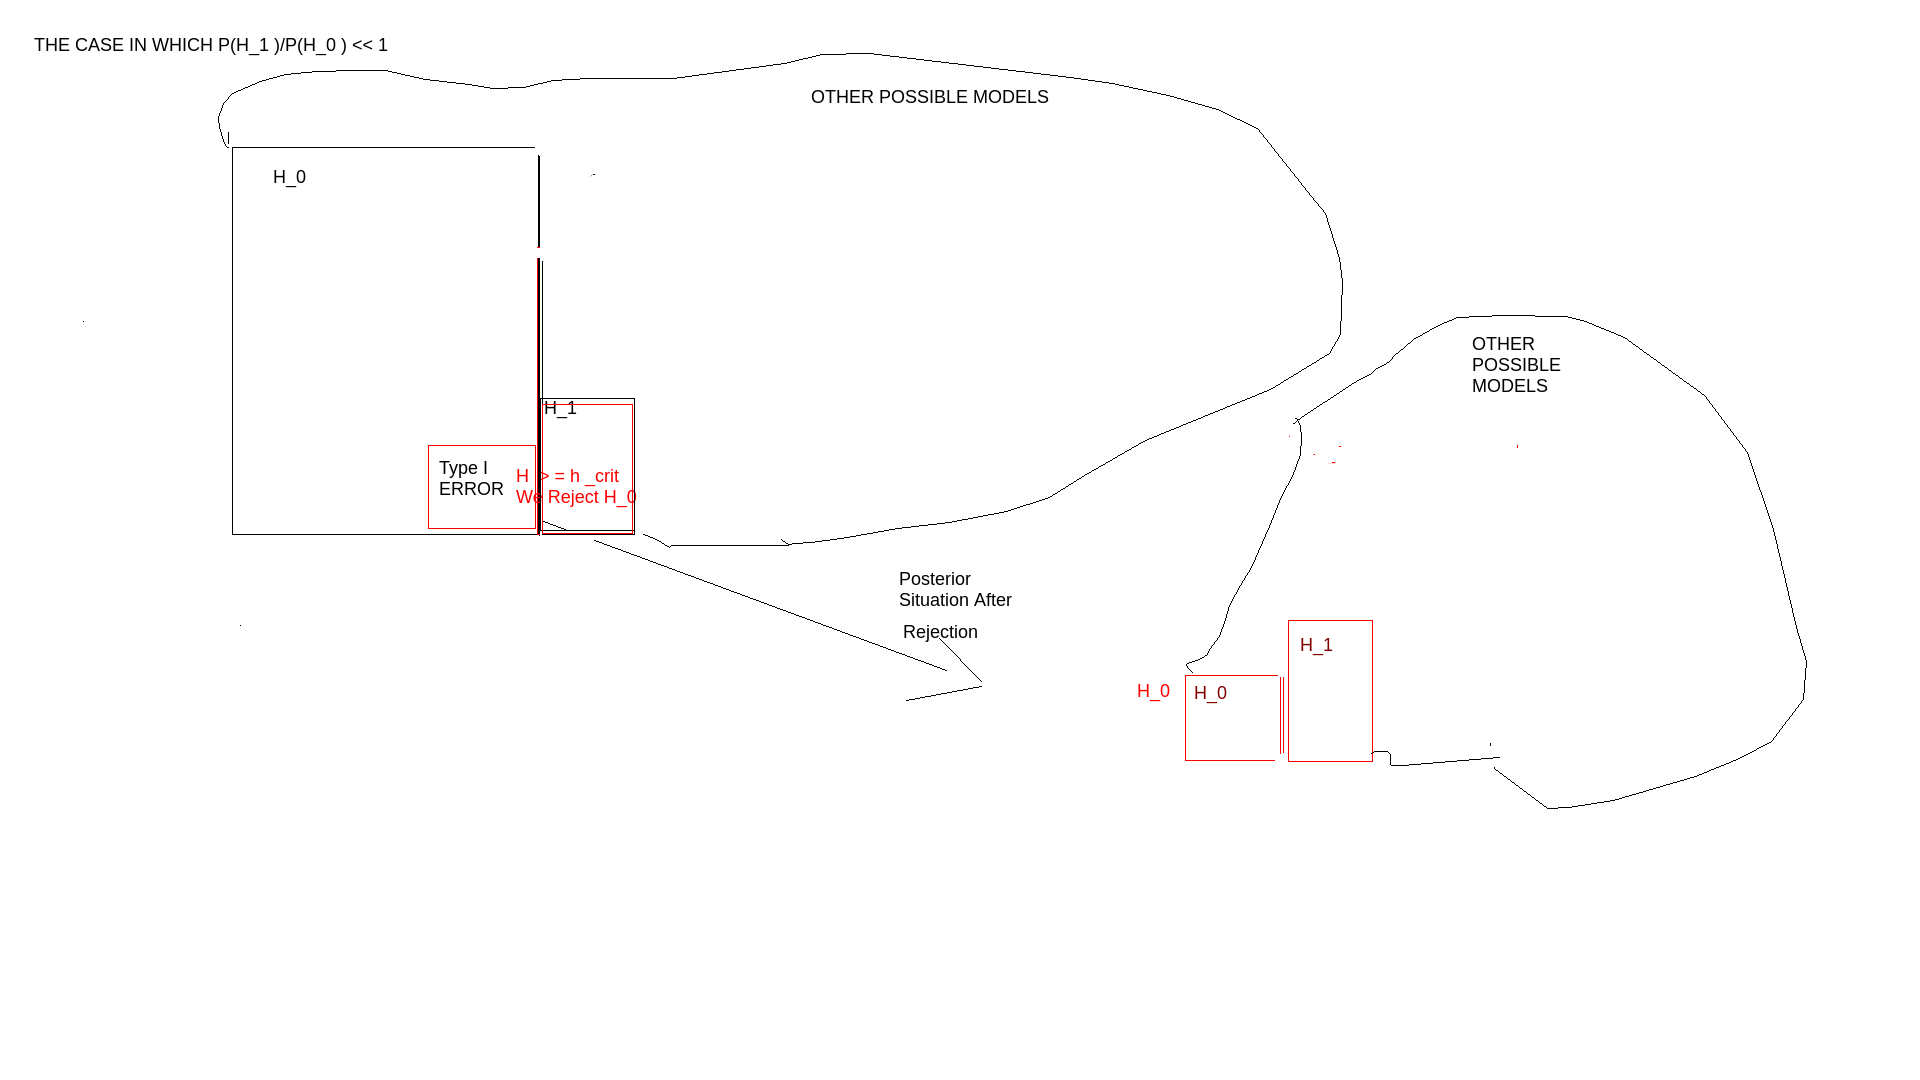
\includegraphics[width=14cm]{posterior_small.png}
	\label{f:posterior_small}
	\end{figure}

	\subsection{ Reviewing some examples}

	\subsection{Homework: te magician}
	\begin{ExerciseList}
	
	
\Exercise \textbf{The magician.}
	 Assume that a person is claiming to have paranormal abilities and that he agrees to have his abilities tested. We prepare a box containing 3 balls, identically in every aspect but color, 2 of them being blue and one of them red. An assistant is then in charge of shuffling the box, extracting a ball randomly, recording its color and reinserting the ball again, and this procedure will be repeated a fixed number of times, and the magician will use its abilities to guess the colour of the balls.   
	
	\Question  \textbf{The best strategy.} What is the best strategy for the magician if he actually doesn't have magicial abilities?
	
	\Question \textbf{ Rephrasing of the experiment into a coin tossing problem} We decide to pick a ball 12 times.  Denoting by $X$ the number of correct guesses, how can you rephrase the problem in terms of coin tosses?
	
	\Question \textbf{ Statement of the hypotheses.} State your null hypothesis and an alternative in terms of the original question and in terms of the coin-tossing model.
	
	\Question \textbf{Distribution of the statistic under $H_0$} Assume that $H_0$ holds, i.e., that he is not a magician. What is the distribution of $X$? 

	\Question \textbf{Decision rule.} To decide whether or not to reject $H_0$ in favour of $H_1$ we consider the statistic of the number of guesses. We decide that if $X \geq X_{\text{crit}}$ for a given threshold $X_{\text{crit}}$, we reject $H_0$ in favour of $H_1$. We fix $X_{\text{crit}} = 12$, that is, we claim that he is a magician if and only if the he guesses correctly 12 times out of 12. Recall that a type I error is the error made when $H_0$ holds but the test rejects it, while a type II error is the error that is made if $H_0$ is not rejected but $H_1$ is true. Compute the type I and the type II error probabilities assuming that $H_0$ holds, i.e., that he is not a magician.  

	\Question \textbf{ Decision rule for a given significance level}
	\Answer We now want to fix the critical level $X_{\text{crit}}$ by fixing in advance the type I error probability provided $H_0$ holds. For $\alpha = 0.05$, find the smallest value of $X_{crit}$ such that probability to make type I error is less than $\alpha$.

\begin{knitrout}
\definecolor{shadecolor}{rgb}{0.969, 0.969, 0.969}\color{fgcolor}\begin{kframe}
\begin{alltt}
\hlcom{# Type I error probability }
\hlkwd{pbinom}\hldef{(}\hlnum{11}\hldef{,} \hlkwc{size} \hldef{=} \hlnum{12}\hldef{,} \hlkwc{prob} \hldef{=} \hlnum{2}\hlopt{/}\hlnum{3}\hldef{,} \hlkwc{lower.tail} \hldef{= F )}
\end{alltt}
\begin{verbatim}
## [1] 0.007707347
\end{verbatim}
\begin{alltt}
\hlcom{# With lower.tail = F, pbinom(k) computes P( X > k | H_0)}
\hldef{(}\hlnum{2}\hlopt{/}\hlnum{3}\hldef{)}\hlopt{^}\hldef{\{}\hlnum{12}\hldef{\}}
\end{alltt}
\begin{verbatim}
## [1] 0.007707347
\end{verbatim}
\begin{alltt}
\hlcom{# The type II error probability is 0, since we are assuming that $H0$ holds}
\hlnum{0}
\end{alltt}
\begin{verbatim}
## [1] 0
\end{verbatim}
\end{kframe}
\end{knitrout}
	\Answer 	
	Under $H_0$ $X$ is a binomial of parameters $n = 12$ and $p = 2/3$. Therefore  
\begin{knitrout}
\definecolor{shadecolor}{rgb}{0.969, 0.969, 0.969}\color{fgcolor}\begin{kframe}
\begin{alltt}
\hldef{size} \hlkwb{<-} \hlnum{12}
\hldef{p} \hlkwb{<-} \hlnum{2}\hlopt{/}\hlnum{3}
\hlcom{## By guessing }
\hlkwd{pbinom}\hldef{(}\hlnum{7}\hlopt{:}\hlnum{11}\hldef{,} \hlkwc{size} \hldef{= size,} \hlkwc{prob} \hldef{=p,}  \hlkwc{lower.tail} \hldef{= F )}
\end{alltt}
\begin{verbatim}
## [1] 0.631520714 0.393074678 0.181122646 0.053951426 0.007707347
\end{verbatim}
\begin{alltt}
\hlcom{## Using the quantile function}
\hlkwd{qbinom}\hldef{(}\hlnum{0.95}\hldef{,}  \hlkwc{size} \hldef{= size,} \hlkwc{prob} \hldef{= p)} \hlopt{+} \hlnum{1}
\end{alltt}
\begin{verbatim}
## [1] 12
\end{verbatim}
\end{kframe}
\end{knitrout}
	\Answer	Let us consider a coin that lands with "head" with probability $p$. Then our null hypothesis and alternative are stated as follows:i
		\bel{}{
			H_0: \, \, p = \frac23 
		}
		\bel{}{
			H_1 \,\, p > \frac23
		}
	
		Note that any $p$ that is larger then theoretically possible $2/3$ constitute violation of null hypothesis: i.e. even if the magician can predict correct result with probability $2/3 + 0.000000001$, he still a magician.
	\end{ExerciseList}
	\section{Law of Large Numbers}

	\subsection{Independent Samples}

	Recall from the definition of distribution function of a random variable X in Definition~\ref{}, and the notion of independent samples from the variable $X$ in Section~\ref{}, which we rewrite below for the sake of clarity. 
		\begin{definition}
				\label{d:sample}
				Let $n\in \mathbb N$ be a number, called the sample size. The random variables $X_1$,...$X_n$ are \emph{independent samples} of $X$ if 
		\begin{itemize}
			\item The $X_i$ are identically distributes, and their common distribution coincides with $p_X$, the one of $X$: for each $a, b \in \mathbb R$ with $a <b$, 
				\begin{equation}
					\label{e:identically}
					\mathbb P(X_1 \in (a,b )) = \ldots = \mathbb P(X_n \in [a,b]) = p_X([a,b])
				\end{equation}
			\item The $X_i$ are independent. For each $a_i, b_i \in \mathbb R$, $i = 1,\ldots, n$ with $a_i \leq b_i$ for every $i$,  
				\begin{equation}
					\label{e:independence}
					\mathbb P( (X_1 \in [a_1, b_1 ], \ldots , X_n \in[a_n, b_n]) = \mathbb P(X_1 \in [a_1, b_1]) \ldots \mathbb P( X_n \in [a_n , b_n]). 
				\end{equation}
		\end{itemize}
		\end{definition}
	We can take samples froma a real population. If we want to make a statistical study on the height of citizens in Moscow we can take intepenendent sample from the actual Moscow population
\begin{knitrout}
\definecolor{shadecolor}{rgb}{0.969, 0.969, 0.969}\color{fgcolor}\begin{kframe}
\begin{alltt}
\hldef{n_moscow} \hlkwb{<-} \hlnum{1000000}
\hldef{Moscow_heights} \hlkwb{<-} \hlnum{10}\hlopt{*}\hlkwd{runif}\hldef{(n_moscow)} \hlopt{+} \hlnum{172}
\hlcom{### The  whole population, that is, the above vector }
\hlcom{### Is unaccessible to us}
\hlcom{### However, we can take samples }
\hldef{sample_size} \hlkwb{=} \hlnum{1000}
\hldef{Sampled_heights} \hlkwb{<-} \hlkwd{sample}\hldef{( Moscow_heights, sample_size )}
\end{alltt}
\end{kframe}
\end{knitrout}
	One can also take independent samples from a distribution, see Definition~\ref{d:sample}. In the following code we take samples from an exponential random variable.
\begin{knitrout}
\definecolor{shadecolor}{rgb}{0.969, 0.969, 0.969}\color{fgcolor}\begin{kframe}
\begin{alltt}
\hldef{sample_size} \hlkwb{<-} \hlnum{10000}
\hldef{Sample} \hlkwb{<-} \hlkwd{rexp}\hldef{(sample_size)}
\hlcom{##### Usually  we don't know that for generating the }
\hlcom{#### sample we used an exponential random variable}
\end{alltt}
\end{kframe}
\end{knitrout}
Note that the two codes are very similar and the only difference is that \textit{ sample( Moscow\_heights,  )} is replaced by \textit{rexp()}. In both cases, for real data, we would like to know the function used to generate the samples, but we have only access to the sample. 
A random variable can be regarded as an abstract population and what we will say applies in the same fashion to both cases, as long as we can take samples. Moreover, sampling from an actual population can be seen as a particular case of sampling from a random variable.
	An exponential random variable is a good model for the living time of objects and you can think that a mobile work decides how long it will work by sampling from the population given by an exponential random variable the total  ammount of time 
	
	\subsection{Statement of the law of large numbers }
	We are interested in computing the mean height of the Moscow population. 
\begin{knitrout}
\definecolor{shadecolor}{rgb}{0.969, 0.969, 0.969}\color{fgcolor}\begin{kframe}
\begin{alltt}
\hldef{n_moscow} \hlkwb{<-} \hlnum{1000000}
\hldef{Mosow_heights} \hlkwb{<-} \hlnum{10}\hlopt{*}\hlkwd{runif}\hldef{(n_moscow)} \hlopt{+} \hlnum{176}
\hlkwd{mean}\hldef{(Moscow_heights)}
\end{alltt}
\begin{verbatim}
## [1] 177.0024
\end{verbatim}
\end{kframe}
\end{knitrout}
	Unfortunately, we do not have access to the whole population and, so that the vector  \textit{Moscow\_heights} and therefore its mean \textit{mean(Moscow\_heights)} are unknown to us. However, it is possible to take independent samples, see Definition~\ref{d:sample}, and we can compute the \textit{sample\_mean} 
\begin{knitrout}
\definecolor{shadecolor}{rgb}{0.969, 0.969, 0.969}\color{fgcolor}\begin{kframe}
\begin{alltt}
\hldef{sample_size} \hlkwb{<-}   \hlnum{1000}
\hldef{sample} \hlkwb{<-} \hlkwd{sample}\hldef{( Moscow_heights , sample_size)}
\hlcom{# Althought we aren't replacing, the samples are almost independent since the sample}
\hlcom{#size is much smaller that the whole population }
\hldef{sample_mean} \hlkwb{<-} \hlkwd{mean}\hldef{(sample)}
\hldef{sample_mean}
\end{alltt}
\begin{verbatim}
## [1] 177.0609
\end{verbatim}
\begin{alltt}
\hlkwd{mean}\hldef{(Moscow_heights)}
\end{alltt}
\begin{verbatim}
## [1] 177.0024
\end{verbatim}
\end{kframe}
\end{knitrout}
	Similar considerations hold when sampling from a generalised population, or a random variable. For a discrete random variable we have defined its mean in Definition~\ref{d:mean}, and the Lebesgue integration procedure allows to extend the definition of mean for generic distribution. Take for instance data on the reaction times to a linguistic stimulus collected in an experiment. They could look in the following way
\begin{knitrout}
\definecolor{shadecolor}{rgb}{0.969, 0.969, 0.969}\color{fgcolor}\begin{kframe}
\begin{alltt}
\hldef{sample_size} \hlkwb{<-} \hlnum{10000}
\hldef{reaction_times} \hlkwb{<-} \hlkwd{rlnorm}\hldef{(sample_size)}
\hlcom{# We are assuming that the reaction times follow an }
\hlcom{# exponential of rate 1. }
\hlcom{# It's mean is 1 }
\hlkwd{mean}\hldef{(reaction_times)}
\end{alltt}
\begin{verbatim}
## [1] 1.630567
\end{verbatim}
\end{kframe}
\end{knitrout}
	Once more, we don't know that to generate the data we used a lognormal distribution(a usual model for reaction time data) of mean, and we have only access to data. 
	What the Law of Large Numbers tells us is that the sample mean is a good approximation of the mean of the population, in the first case, and of the random variable, in the second. 

	\begin{definition}[Sample mean for a random variable]
		\label{d:sample_mean} Let $p_X$ be a distribution of a random variable $X$ with a well defined mean $\mu$, and let  $\underline X = (X_1, \ldots, X_n)$ be samples from $X$. The sample mean is   
			\begin{equation}
				\label{e:sample_mean_x}
				m(\underline X ) = \frac{X_1 + \ldots + X_n }{n}
			\end{equation}
	\end{definition}
	Similarly, $m(\underline X)$ can be defined also for samples from a population. The Law of Large Numbers tells us that 
	\begin{theorem}[Strong Law of Large Numbers ]
		Let $X$ be a distribution with a well defined mean $\mu$ and let $\underline X = (X_1 , \ldots )$ be independent samples form $X$. Then 
			\begin{equation}
			m_(\underline X) \coloneq \frac{X_1 + \ldots + X_n}{n} \to \mu
			\end{equation}
	\end{theorem}
	Note that the random quantity on the left hand side, is converging to a deterministic constant. 
	
	\subsection{ Dependence from the Sample Size}
		
	One could study the Law of Large Numbers in more detail and provide some \emph{quantitative} version of it: we can tell how good, depending on the sample size, the approximation of the real mean by the sample mean is. Instead, we plot some graphs to visualize the dependence of the smaèple mean from the sample size
\begin{knitrout}
\definecolor{shadecolor}{rgb}{0.969, 0.969, 0.969}\color{fgcolor}\begin{kframe}
\begin{alltt}
\hldef{n_moscow} \hlkwb{<-} \hlnum{1000000}
\hldef{Moscow_heights} \hlkwb{<-} \hlnum{10}\hlopt{*}\hlkwd{runif}\hldef{(n_moscow)} \hlopt{+} \hlnum{172}
\hldef{sample_size} \hlkwb{<-} \hlnum{10000}
\hldef{Sampled_heights} \hlkwb{<-} \hlkwd{sample}\hldef{(Moscow_heights, sample_size)}
\hldef{sample_mean} \hlkwb{<-} \hlkwd{cumsum}\hldef{(Sampled_heights)}\hlopt{/}\hlnum{1}\hlopt{:}\hldef{sample_size}
\hlkwd{ggplot}\hldef{(}\hlkwc{data} \hldef{=} \hlkwd{tibble}\hldef{(}\hlkwc{x} \hldef{=} \hlnum{1}\hlopt{:}\hldef{sample_size,} \hlkwc{y} \hldef{= sample_mean),} \hlkwd{aes}\hldef{( x, y))} \hlopt{+}
        \hlkwd{geom_line}\hldef{()}\hlopt{+}
        \hlkwd{geom_hline}\hldef{(} \hlkwc{yintercept} \hldef{=} \hlkwd{mean}\hldef{(Moscow_heights),} \hlkwc{col} \hldef{=}\hlsng{'red'}\hldef{)}
\end{alltt}


{\ttfamily\noindent\bfseries\color{errorcolor}{\#\# Error in ggplot(data = tibble(x = 1:sample\_size, y = sample\_mean), aes(x, : non trovo la funzione "{}ggplot"{}}}\end{kframe}
\end{knitrout}

Similarly for the reaction time experiment 
		
\begin{knitrout}
\definecolor{shadecolor}{rgb}{0.969, 0.969, 0.969}\color{fgcolor}\begin{kframe}
\begin{alltt}
\hldef{sample_size} \hlkwb{<-} \hlnum{10000}
\hldef{reaction_times} \hlkwb{<-} \hlkwd{rexp}\hldef{(sample_size)}
\hlcom{# We are assuming that the reaction times follow an }
\hlcom{# exponential of rate 1. }
\hlcom{# It's mean is 1 )}
\hldef{mu} \hlkwb{=} \hlnum{1}
\hldef{sample_mean} \hlkwb{<-} \hlkwd{cumsum}\hldef{(reaction_times)}\hlopt{/}\hlnum{1}\hlopt{:}\hldef{sample_size}
\hlkwd{ggplot}\hldef{(}\hlkwc{data} \hldef{=} \hlkwd{tibble}\hldef{(}\hlkwc{x} \hldef{=} \hlnum{1}\hlopt{:}\hldef{sample_size,} \hlkwc{y} \hldef{= sample_mean),} \hlkwd{aes}\hldef{( x, y))} \hlopt{+}
        \hlkwd{geom_line}\hldef{()}\hlopt{+}
        \hlkwd{geom_hline}\hldef{(} \hlkwc{yintercept} \hldef{= mu ,} \hlkwc{col} \hldef{=}\hlsng{'red'}\hldef{)}
\end{alltt}


{\ttfamily\noindent\bfseries\color{errorcolor}{\#\# Error in ggplot(data = tibble(x = 1:sample\_size, y = sample\_mean), aes(x, : non trovo la funzione "{}ggplot"{}}}\end{kframe}
\end{knitrout}

	\section{ Empirical distribution}

	In this section we show that, as a corollary of the Law of Large Numbers~\ref{t:LLN}, it is the same to know the distribution of a random variable $X$ and to be able to take independent samples from it. In particular, we shoe that from the histogram of the sampled values we are able to recover the distribution of $X$. This is often taken as a basis in the frequentist interpretation of probability, but it is a result and it is not always possible to take independent samples 

		\subsection{Estimation of the parameters of the Bernoulli trials model }
		\begin{example}[Estimation of the $p$ in Bernoulli trials]
			\label{ex:estimate_Bernoulli}	Consider a string $\underline X$ whose digits $X_i$, for $i = 1 , \ldots, n$, $n \in \mathbb N$,  are either $0$ or $1$, and assume we have observe $x_1x_2 \ldots x_n $. We use the model of Bernoulli trials $\mc Q = \{\mathbb P_p, p \in [0,1]\}$, see Definition~\ref{}, so that we assume that $\underline X$ distributes according to $\mathbb P_p$ for some $p$. To estimate it, we notice that
	\bel{e:p_as_mean}{
		p = \mathbb E[X_i] \qquad \text{for each $i =1, \ldots, n$ }, 
	} 
	and the law of large numbers, toghether?? with the independence assumption of the digits that each $\mathbb P_p \in  \mathcal Q$ possesses, guarantees that
	\bel{}{
		\frac{X_1 + \ldots + X_n }{n } \to p 
	}  
	\end{example}
	\begin{example}[Estimation of the distribution]
		Let $X_i$,  for $i = 1, \ldots $,  be independent samples from a distribution $X$. In this example we show that it is the same to know the distribution of $X$, $\mathbb P_X$, see~\ref{d:distribution} or the sample $X_i$, $i = 1, \ldots$. Indeed, define    
		\bel{e:indicator_set}{
			Y_{[a,b]}  = \begin{cases}
			1 & \text{ if $X_i \in [a, b]$ }\\
			0 & \text{otherwise}
			\end{cases} 
		}
		It is intuitive, and indeed(Maybe add a proof on how to show that two Bernoulli are independent in ther independence section???) it can be proved, that the $Y_i$ are independent, since they are function of $X_i$ alone, for each $i  = 1, \ldots, n$. Therefore the $Y_i$ form a sequence of Bernoulli trials and we can apply the Law of Large Numbers in the form of \eqref{e:p_as_mean} that guarantees 
	\bel{}{
		\frac{Y_1 + \ldots + Y_n }{n} \to p
	}  
	where $p$ is the mean of $Y_i$, for each $i$. Since the equality of events $(Y_i = 1 ) = (X \in [a,b])$ holds, 
	\bel{}{
		p = \mathbb E\left[ Y_i\right] = \mathbb P(Y_i = 1 ) = \mathbb P(X_i \in [a,b]) = \mathbb P_X([a,b])
	} 
	so that 
	\bel{e:equality1}{
		\frac{Y_1 + \ldots + Y_n}{ n }\to \mathbb P(X \in [a,b]).
	}
	We further note that the left hand side of the \eqref{e:equality1} is the proportion of the number of $X_i$ that fall in the interval $[a, b]$. We can rewrite everything in the more suggestive form	
	\bel{}{
		\frac{\# \text{of $i$ such that $X_i \in [a,b]$ }}{n} \to \mathbb P_X([a,b]).
	}   
	The above is often mistakenly taken as the definition of probability in the frequentist setting.   
	\end{example}
	
	\begin{example}[Estimation of the parameters of the Markov model ]
		Consider the Markov model $\mathcal Q =\{\mathbb P_{a,b}\}$ introduced in \eqref{e:} for sequences of 0s and 1s, namely we assume that the  observed the string $s_1x_2, \ldots x_n$, $n \in \mathbb N$, $x_i \in \{0,1\}$ for each $i = 1,\ldots,n$, is an instance of the distribution $\mathbb P_{a,b}$. The aim is to estimate the parameters $a$, the probability of jumping to 1 while at 0, and $b$, the probability of jumping from to 0 while at 1,  using the Law of Lerge Numbers. To this end let $n_0$ be the number of 0s in the string $x_1x_2\ldots x_n$ and $n_1$ the number of 1s, and denote, for $i = 1, \ldots,n_0$, $\alpha(i)$ the position of the $i$-th 0, and, for $j = 1, \ldots, n_1$, by $\beta(j)$ the position of the t$j$-th 1. For the sake of concreteness, if we observe 100111000, then $n_0 = 5$, $n_1 = 4$ and $\alpha(1) = 2$, $\alpha(2) = 3$, $\alpha(3) = 7$, $\alpha(4) = 8$, $\alpha(5) = 9$, $\beta(1) = 1$, $\beta(2) =4$, $\beta(3) = 5$ and $\beta(4) = 6$. We then define the two variables   
	\bel{}{
		Y_i = \begin{cases}
			1 & \text{if $X_{\alpha(i)+ 1} = 1$ }\\
			0 & \text{otherwise} 
		\end{cases} 
	}
	and
	\bel{}{
		Z_j = \begin{cases}
			1 & \text{if $X_{\beta(j) + 1 } = 0$, }\\
			0 & \text{otherwise}
		\end{cases}
	}  	
	for $i = 1, \ldots n_0$ and $j = 1, \ldots, n_1$. The variables $Y_i$ indicate if after the $i$-th 0 there is a 1 or a 0, while the variables $Z_j$ indicate whether after the $j$-th 1 there is a 0 or a 1. They are Bernoulli random variables of parameter 
	\bel{}{
		\mathbb P_{a,b}( Y_i = 1 ) &= \mathbb P_{a,b}( X_{\alpha(i) + 1} = 1) = \mathbb P_{a,b}( X_{\alpha(i ) + 1} = 1 , X_{\alpha(i)}  = 0 ) \\
		& = \mathbb P_{a,b}( X_{\alpha(i)} = 1 | X_{\alpha(i)} = 0) = a
	}  
	and  
	\bel{}{
		\mathbb P_{a,b}( Z_j = 1 ) &= \mathbb P_{a,b}( X_{\beta(j) + 1} = 0) = \mathbb P_{a,b}( X_{\beta(j ) + 1} = 0 , X_{\beta(j)}  = 1 ) \\
		& = \mathbb P_{a,b}( X_{\beta(j)} = 0 | X_{\beta(j)} = 0) = b,
	}  
	for each $i = 1, \ldots, n_0$ and $j = 1, \ldots, n_1$, where we have used the strong Markov property and the fact that $X_{\alpha(i)} \equiv 0$ and $X_{\beta(j)}\equiv 1$, by definition of $\alpha$ and $\beta$. They are also independent (maybe in the section independence put how to check whether two Bernoulli are independent???) Let's check some of the pairwise independence.    
	\bel{}{
		\mathbb P( Z_i = 1, Y_j = 1 ) = \mathbb P( X_{\alpha(i ) + 1} = 0 , X_{\alpha(i)} = 1 , X_{\beta(j) + 1 }= 1, X_{\beta(j)} = 0  ) = \mathbb P()
	}
	since $X_{\alpha(i) } = 0$ and $X_{\beta(j)}\equiv 1$ (I am using the strong Markov property, the randomness here is in the functions $\alpha$ and $\beta$)
	Therefore, both $Y_i$ and $Z_j$ form Bernoulli trials of parameter $a$ ans $b$, repsectively, and we can use \eqref{e:p_as_mean} to estimate
	\bel{e:Markov_estimate}{
		&\frac{Y_1 + \ldots + Y_{n_0}}{n_0}\to a \\
		& \frac{Z_1 + \ldots  +Z_{n_1}}{n_1 }\to b
	}  
	Finally we see that on the left hand side in the above equality there is the proportion of jumps from 0 to 1 and to 1 to 0, respectively 
	\end{example}
	

	
	\begin{example}[Montecarlo]
		\label{ex:montecarlo}
		Given $X_i$, $i = 1, \ldots$, independent samples from a distribution $\mathbb P_X$, we can estimat $\mathbb E[f(X)]$, see Defintion~\ref{d:expected}, using the Law of Large Numbers. The random variables $f(X_i)$, $i =1, \ldots, n$ can be seen to be independent (since $f(X_i)$ depends only on $X_i$ and none other, and the $X_i$ are independent), so that the Law of Large Numbers~\ref{t:LLN} applies
		\bel{e:montecarlo}{
		\frac{f(X_1) + \ldots + f(X_n)}{n }\to \mathbb E\left[f(X)\right]
	}    
	\end{example}
	\begin{example}[Estimation of the standard deviation of the distribution]
		\label{ex:montecarlo_variance}
		Let $X_i$, $i = 1, \ldots$ , be independent samples from a distribution $\mathbb P_X$ of mean $\mu$. Applying Example~\ref{ex:montecarlo} to the function $f(x) = (x - \mu)^2$, we can estimate the variance of $\mathbb P_X$ by   
		\bel{e:montecarlo_variance}{
			\frac{(X_1 - \mu)^2+ \ldots + (X_n - \mu)^2}{n} \to \mathbb E\left[( X - \mu)^2\right]	 = \text{Var}(X)
		}   
	\end{example}

		\subsection{ Histograms and empirical distributions}
		\label{ss:histogram}
		Assume we have collected some continuous data $\underline X = (X_1, \ldots, X_n)$ associated to the variable $X$. An histogram is a way to visualise the data that requires to specify 
		\begin{itemize}
			\item A vector $\underline X$ with the data  
			\item A vector of breaks that specify intervals in the $x$-axis. For instance, the vector \textit{ breaks = c(1,3,5)} specifies the intervals $(-\infty, 1]$,$[1,3]$, $[3,5]$ and $[5, +\infty)$. 
			\item A specification of what needs to be plotted in the $y$ axis. It could be the total frequency of the data, that is, the height vertical bar associated to the base segment $[a,b]$ is the total frequency of $X_i$ falling in the interval $[a,b]$.   
		\end{itemize}

	We can easily plot the histogram associated to samples from the exponential distribution, defined by $\mathbb P(X \in [a,b])) = \int_{\max\{a,0\}}^{\max\{b,0\}} e^{-x} dx$.

\begin{knitrout}
\definecolor{shadecolor}{rgb}{0.969, 0.969, 0.969}\color{fgcolor}\begin{kframe}
\begin{alltt}
\hlkwd{library}\hldef{(}\hlsng{'tidyverse'}\hldef{)}
\end{alltt}


{\ttfamily\noindent\itshape\color{messagecolor}{\#\# -- Attaching core tidyverse packages ---------------------------------------------------------------------------------------------------------------------------------------------------- tidyverse 2.0.0 --\\\#\# v dplyr \ \ \ \ 1.1.4 \ \ \ \ v readr \ \ \ \ 2.1.5\\\#\# v forcats \ \ 1.0.0 \ \ \ \ v stringr \ \ 1.5.1\\\#\# v ggplot2 \ \ 3.5.2 \ \ \ \ v tibble \ \ \ 3.3.0\\\#\# v lubridate 1.9.4 \ \ \ \ v tidyr \ \ \ \ 1.3.1\\\#\# v purrr \ \ \ \ 1.0.4 \ \ \ \ \\\#\# -- Conflicts ---------------------------------------------------------------------------------------------------------------------------------------------------------------------- tidyverse\_conflicts() --\\\#\# x dplyr::filter() masks stats::filter()\\\#\# x dplyr::lag() \ \ \ masks stats::lag()\\\#\# i Use the conflicted package (<http://conflicted.r-lib.org/>) to force all conflicts to become errors}}\begin{alltt}
\hldef{sample_size} \hlkwb{<-} \hlnum{100000}
\hldef{data} \hlkwb{<-} \hlkwd{rexp}\hldef{(sample_size)}
\hlcom{## breaks is the vector of the endpoints of the segments in the xx axis }
\hldef{breaks}  \hlkwb{<-} \hlkwd{c}\hldef{(}\hlnum{0}\hldef{,}\hlnum{0.2}\hldef{,}\hlnum{0.4}\hldef{,}\hlnum{0.6}\hldef{,} \hlnum{1}\hldef{,} \hlnum{1.5}\hldef{,}\hlnum{3.5} \hldef{,} \hlnum{5}\hldef{)}
\hlkwd{ggplot}\hldef{(} \hlkwc{data} \hldef{=} \hlkwd{tibble}\hldef{(} \hlkwc{x} \hldef{= data ))} \hlopt{+}
        \hlkwd{geom_histogram}\hldef{(} \hlkwd{aes}\hldef{( x ),} \hlkwc{breaks} \hldef{= breaks )}
\end{alltt}
\end{kframe}
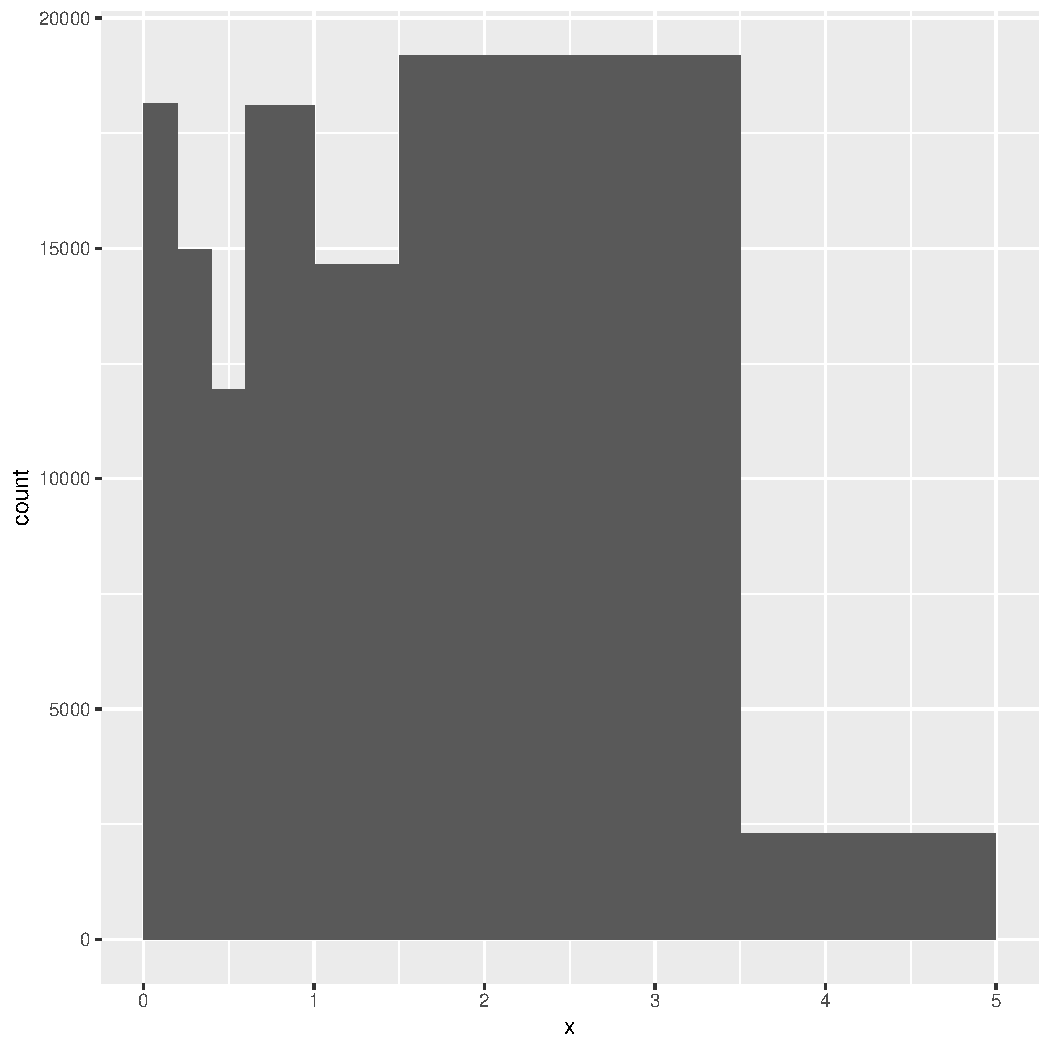
\includegraphics[width=\maxwidth]{images/statistics//histogram_frequencies-1} 
\end{knitrout}

	One of the consequence of the Law of Large numbers that we wish to outline is that kmowing the distribution and knowing how to take an arbitraty number of samples is the same thing. Indeed, let $[a,b]$ be an interval with $a \leq b$ and define the random variable $Y_i$ that indicates whether or not $X_i$ lies in the interval $[a,b]$: 
		\begin{equation}
			\label{e:indicator}
			Y_i
			\begin{cases}
				1 & \text{ if } X_i \in [a,b]\\
				0 & \text{ otherwise }
			\end{cases}
		\end{equation}
		The $Y_i$ are independent since the $X_i$ are and the mean of $Y_i$ is $\mathbb P( X \in [a,b])$. The Law of Large Numbers implies that 
		\begin{equation}
			\label{e:sample=distr}
			\frac{Y_1 + \ldots + Y_n}{n} \to \mathbb P(X \in [a,b])
		\end{equation}
		as $n$ gets bigger. 
		The above fact is useful to better understand the histogram. Indeed, if $[a,b]$ is an interval in the $x$ axis of the histogram, then $(Y_1 + \ldots + Y_n)/n$ is the height of the histogram bar plotting the relative frequencies. Therefore plotting the histogram of the relative frequenies is a good way to represent the distribution of a random variable, which is at the basis of the problematic frequentist interpretation of Probability Theory

	Denote $[a_i,b_i]$ the base intervals of the histogram. The approximation \eqref{e:sample=distr} is good as soon as $n >> \frac{1}{\mathbb P(X \in [a_i,b_i])}$. Therefore, the histogram is a good approximation of the distribution if $n >>1/p_X([a_i,b_i])$ for each $i =1,\ldots, k $, where $k$ is the number of bins in the histogram. Moreover, if one wants to have small intervals on the x-axis we should take $k$ large. Therefore to give a good representation of the distribution we should have $n >> k>> 1$, where $n>>k$ is needed to apply the Law of Large Numbers to each interval, and $k >>1$ is needed to have small intervals. 
		
		\begin{example}[Density histogram]
			As the intervals $[a_i,b_i]$ shrink, the relative frequency of each interval decreases (unless we are dealing with discrete random variables, see Definition~\ref{d:random_variable}) Next we show that for continuous random variables it is useful to plot the density histogram, especially when $[a,b]$ is small. Continuous random variable are characterised by the fact that they have a \emph{density} funciton $f$, that is, a function $f$ verifying  $\mathbb P(X \in [a, b]) = \int_a^b f(x) dx$. If the interval $[a,b]$ is small then $ \int_a^b f(x) dx \sim f(a)(b - a)$ (we are also assuming that $f$ is continuous) and we have 
				\begin{equation}
					\label{e:int_approx}
					\mathbb P(X \in [a,b]) \sim f(a) (b-a)
				\end{equation} 
				(we are assuming $f$ continuous in $a$) is a good approximation. Plotting the histogram of the density, which is equal to the relaitive frequency divided by the length of the base segment, gives  a good approximation of the density function: 
				\begin{equation}
				\frac{Y_1 + \ldots + Y_n}{n(b-a)} \to \frac{\mathbb P(X \in [a,b])}{(b-a)}  \sim f(a)
				\end{equation}
				Once more, $n >> k$ since for each interval $[a_i,b_i]$ we need $ n >> 1/p_X([a_i,b_i])$ to apply the Law of Large Numbers, and in order to apply \eqref{e:int_approx} we need $b_i - a_i$ small for each $i$, and therefore $k >>1$, where $k$ is the number of intervals

\begin{knitrout}
\definecolor{shadecolor}{rgb}{0.969, 0.969, 0.969}\color{fgcolor}\begin{kframe}
\begin{alltt}
\hldef{sample_size} \hlkwb{<-} \hlnum{1000000}
\hldef{number_bins} \hlkwb{<-} \hlnum{1000}
\hldef{data} \hlkwb{<-} \hlkwd{rexp}\hldef{(sample_size)}
\hlkwd{ggplot}\hldef{(} \hlkwc{data} \hldef{=} \hlkwd{tibble}\hldef{(}\hlkwc{x} \hldef{= data ))} \hlopt{+}
        \hlkwd{geom_histogram}\hldef{(} \hlkwd{aes}\hldef{( x ,} \hlkwc{y} \hldef{=} \hlkwd{after_stat}\hldef{(density)),} \hlkwc{bins} \hldef{= number_bins)} \hlopt{+}
        \hlkwd{stat_function}\hldef{(} \hlkwc{fun} \hldef{= dexp ,} \hlkwc{args} \hldef{=} \hlkwd{list}\hldef{(}\hlkwc{rate} \hldef{=} \hlnum{1}\hldef{),} \hlkwc{col} \hldef{=} \hlsng{'red'}\hldef{)}
\end{alltt}
\end{kframe}
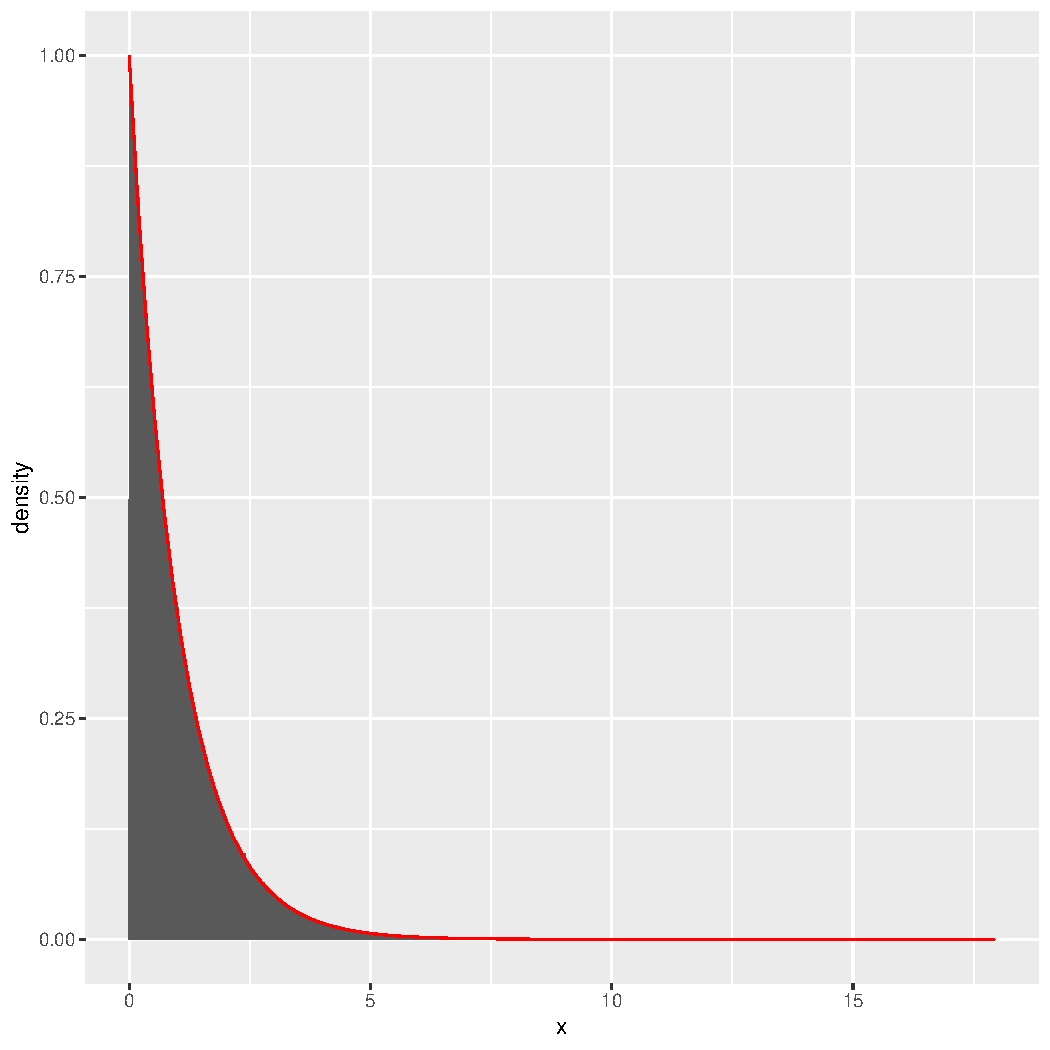
\includegraphics[width=\maxwidth]{images/statistics//Histogram_density-1} 
\end{knitrout}
	\end{example}

	Here we comment of the fact that the great majority of distributions are neither continuous nor discrete. 
	\eqref{e:int_approx} can be seen as a characterization of coninuous distributions: no matter how small is the interval $[a,b ]$, the probability of $X$ being in that interval is proportional to the length of the interval: 
			\begin{equation}
				\label{e:density_eps}
				\mathbb P(X \in [c- \varepsilon, c + \varepsilon]) = \int_{c - \varepsilon}^{c + \varepsilon} f(x)dx \sim f(c) 2\varepsilon 
			\end{equation}
	This is of course not true for discrete random variables, see Defnition~\ref{d:discrete}. Think at a Bernoulli random variable and take $c = 0$. Then the probability of obtaining a point in $[- \varepsilon, \varepsilon ]$ is $\mathbb P( X \in [-\varepsilon, \varepsilon ] ) = 1-p$, which is not small or proportional to $(2\varepsilon)$. However, the support of the distribution, that is, the places where the $X$ can be found are only two points, that is, $X$ concentrates in a set of dimension 0.  In general there is a balance on the dimension of the set where the points concentrate and the how much is probable to find points on the set where they concentrate: 
	\begin{equation}
		\mathbb P( X \in [c - \varepsilon , c + \varepsilon ]) \sim f(c) (2\varepsilon )^\delta 
	\end{equation}
	and the function $f$ is different from zero only on a set of fractal dimension $\delta \in [0,1]$. The case $\delta =0$ corresponds to the discrete case, while the case $\delta = 1$ corresponds to the continuous random variables. All the other cases correspond to strange but typical distributions. An example owith $\delta = 2/3$, where the function $f$ has its support on the Cantor set, a set of fractal dimension $2/3$, is given by the the "devil's staircase". In this case, for retrieving $f$, we should divide the relative frequencies not by the length of the base interval but by the length to the power $\delta$ (Indeed, in the discrete case we divide by $1 = (b-a)^0$ ) ( The devil's staircase  corresponds to the uniform distribution on the Cantor set, which consists on the numbers in $[0,1]$ whose ternary expression does not contain the digit 1)

	\begin{ExerciseList}
		\Exercise Fix a degree of precision $k \in \mathbb N$ and sample  $(a_1,\ldots, a_k)$, digits that can be either 0 oro 2 with the same probability. Define the number $x = a_1 3^{-1} + a_2 3^{-2}  + \ldots + a_k 3^{-k}$, that is, use the digits as the digits of the ternary expression of $x$. The number thus obtained is sampled with a distribution that, as $k\to \infty$ is similar to the Cantor one. 
		%\Question Replicate the procedure $n$ times to obtain the histogram of the frequencies\\
		%\Question Show that to obtain the heights is such a way that the order of magnitude does not depend on $n$ you should divide by the relative frequencies by the base of the interval to the power $2/3$. 	
	\end{ExerciseList}
	\section{Exercises}

	In this homework we are going to take a look back into the general framework, see Section~\ref{} of testing and define one to see what it is possible to do when point . In this case we can use the Law of Large Numbers, see Theorem~\ref{}, or, more specifically, Example~\ref{e}, and replace the true distributio

	\subsection{Application to testing}
		In many cases the statistic defined for a test, see \ref{item:statistic} whose extremal values give an hint in favour of $H_1$, is not known explicitely, but it can be simulated. We use the results in \
	\begin{example}[Eugene Onegin 4: Simulating the Statistic under the Null]
		\label{ex:Eugene_Onegin3}
		
	\end{example}
	\section{Eugene Onegin Central Limit Theorem for Markov Chains}
		\begin{theorem}[LLN and CLT for Markov Chain]
		Let $\underline X = X_1 \ldots $ a string of 0s and 1s that distributes according to $\mathbb P_{a,b}$. Then the Law of Large numbers 
		\bel{e:LLN_Marko_Chain }{
			\frac{X_1 + \ldots + X_n}{n} \to p 
		}
		holds with $p = b/(a + b)$. The Central limit theorem holds with a standard deviation 
		\bel{e:sd_markov}{
		\sigma_{\text{Markov}} = \frac{ab(2 - a- b)}{(a + b)^3},
		}
		 namely
		\bel{e:CLT_markov}{
		\sqrt{n} \frac{\tfrac{1}{n} (X_1 + \ldots + X_n) - p }{\sigma_{\text{Markov}}} \to Z
		} 
		where $Z \sim \mc N(0,1)$ is a standard normal.  	
		\end{theorem}
	We rapidy check the above two theorems by repeating the same plots of Subection~\ref{} for the Law od Large Numbers and of Subsection~\ref{} for the Central Limit Theorem, substituting the fujnction rbinom with the function defined in Subsection~\ref{} \textit{simulate\_markov\_chain}, and wisn 
	\textbf{ The Law of Large Numbers }

	\textbf{ The Central Limit Theorem}

	We want to check that the sequence of 0s and 1s saved in the vector \textit{text\_01} satisfies the CLT with the variance $\sigma_{\text{Markov}}$ rather than the one that predicted by the CLT~\ref{t:CLT}, $\sigma = \sqrt{p(1-p)}$, see also Example~\ref{}. In this way we conclude that $H_1$ is (way) more likely to be true.    
	To this end, we choose $n$ big enough so that 
	\bel{e:CLT_statistic}{
		z(X_1, \ldots, X_n) = \sqrt{n} \left(\frac{1}{n} \left(X_1 + \ldots + X_n\right) - p \right)
	}
	approximates a Gaussian of standard deviation $\sqrt{p(1-p)}$ if $X_1\ldots X_n$ follows a Bernoulli measure or a Gaussian of standard deviation $\sigma{\text{Markov}}$, if $H_1$ holds. We then separate the vector \textit{text\_01} into many chunks of length $n$: $a_1 = X_1X_2\ldots X_n$, $a_2 \underline X_{n+1}\ldots X_{2n}$...
	We then compute on for each of this chuncks the statistic \eqref{e:CLTstatistic}
	\bel{e:many_z}{
	z_i = z(X_{i*n + 1 }, \ldots , X_{(i+1)*n})
	}
	 and we use the result of Example~\ref{e:} to simulate the distribution of $z$. Notice that we are making the assumption that the $z_is$ are independent, which not true. since the different chunks are not independent. However, the dependence between $z_i$ comes from the boundary terms, that is, form the terms $X_{i*n + 1}$, $X_{i*n + n-1 }$ which are much less than $\sqrt{n}$, and since each of the $X_{i*n+ j}$ enters in the definition of $z_i$ divided by $\sqrt{n}$, it is not a big assumption. 
	Therefore, the histogram and we can check graphically that 
   
	\subsection{ Homework: The Magician Strikes Back}
	
	Credits: Exercise taken from \url{<http://math-info.hse.ru/2019-20/Linguistic_Data:_Quantitative_Analysis_and_Visualisation:_linguistic_theory>}
	
	\begin{ExerciseList}
 	
		\Exercise Problem 2: the magician and the mean
		The magician of Subsection~\ref{} is claiming to have psycokinetic abilities. To test them we agree to perform the following experiment. In a box we place 5 balls, indentical to one another with the exception that each ball has a number on it: 1, 3, 4, 7, 8. We select random ball, record the number, put the ball again in the box, shuffle the balls and repeat the process several times obtaining a sample. The magician uses his abilities to make average of these numbers to be as large as possible.

	\Question  \textbf{Population mean} Find population mean, i.e. average of numbers in the box.


	\Question \textbf{ Sample mean vs. population mean}

Assume that at some experiment we obtained the following sample: 8, 3, 3, 1, 1, 7, 8, 7. Its mean (find it) is larger than the population mean. The magician says:
 Now you see? I has psychokinetic abilities! I said I will increase the mean and it is indeed larger than the population mean. Though 


	\Question \textbf{More results}

Assume that you obtained sample mean that is equal to 8 and your sample size is 5. Does it look convincing now?


 	\Question \textbf{Hypotheses}  State null hypothesis and an alternative in this experiment.
	\Question \textbf{ The decision rule} As the magician claims that he is trying to make the sample mean as large as possible, we use the following decision rule: we choose some value $\bar x_{crit}$ and will claim that the magician has magical abilities if sample average is equal to $\bar x_{crit}$ or larger. Let $\bar x_{crit}=7$. Assume that the magician doesn't have magical abilities. Simulate 10000 sampling from our box, sample size = 5. How many times would you reject null hypothesis, i.e. claim that the magician indeed has magical abilities?


	\Answer
\begin{knitrout}
\definecolor{shadecolor}{rgb}{0.969, 0.969, 0.969}\color{fgcolor}\begin{kframe}
\begin{alltt}
\hldef{population} \hlkwb{<-} \hlkwd{c}\hldef{(}\hlnum{1}\hldef{,}\hlnum{3}\hldef{,}\hlnum{4}\hldef{,}\hlnum{7}\hldef{,}\hlnum{8}\hldef{)}
\hlkwd{mean}\hldef{(population)}
\end{alltt}
\begin{verbatim}
## [1] 4.6
\end{verbatim}
\end{kframe}
\end{knitrout}
\begin{knitrout}
\definecolor{shadecolor}{rgb}{0.969, 0.969, 0.969}\color{fgcolor}\begin{kframe}
\begin{alltt}
\hldef{sample} \hlkwb{<-} \hlkwd{c}\hldef{(}\hlnum{8}\hldef{,}\hlnum{3}\hldef{,}\hlnum{3}\hldef{,}\hlnum{1}\hldef{,}\hlnum{1}\hldef{,}\hlnum{7}\hldef{,}\hlnum{8}\hldef{,}\hlnum{7}\hldef{)}
\hlkwd{mean}\hldef{(sample)}
\end{alltt}
\begin{verbatim}
## [1] 4.75
\end{verbatim}
\end{kframe}
\end{knitrout}

the output doesn't look so different from an output that would have arisen under $H_0$ 
	\Answer
	Yes, If $H_0$ were true this result would be possible only if we select 5 times out of five the ball with an 8  
	
	\Answer
$H_0$: $X$ is the mean of random extractions from the urn. 
$H_1$: $X$ follows a distribution with mean $\mu > 4.6 $
Note that the following step is crucial to compute the distribution of $X$ if $H_0$ were true 
	\Answer
\begin{knitrout}
\definecolor{shadecolor}{rgb}{0.969, 0.969, 0.969}\color{fgcolor}\begin{kframe}
\begin{alltt}
\hlcom{## Although one could theoretically compute the distribution of $X$ given $H_0$, for instance P(X = 8 ) = (1/5)^5, the computations are too long. This step i srequired if the  distribution of $X$ given $H_0$ is not known explicitely }
\hldef{k} \hlkwb{<-} \hlnum{1000}
\hldef{many_sampled_X} \hlkwb{<-} \hlkwd{replicate}\hldef{(k,} \hlkwd{mean}\hldef{(}\hlkwd{sample}\hldef{(}\hlkwc{size} \hldef{=} \hlnum{5}\hldef{,} \hlkwc{x} \hldef{= population,} \hlkwc{replace} \hldef{= T )))}
\hlcom{## mean(sample(size = 5, x = population, replace = T )) computes an observation of X, and I replicate it k times }
\hlkwd{hist}\hldef{(many_sampled_X)}
\end{alltt}
\end{kframe}
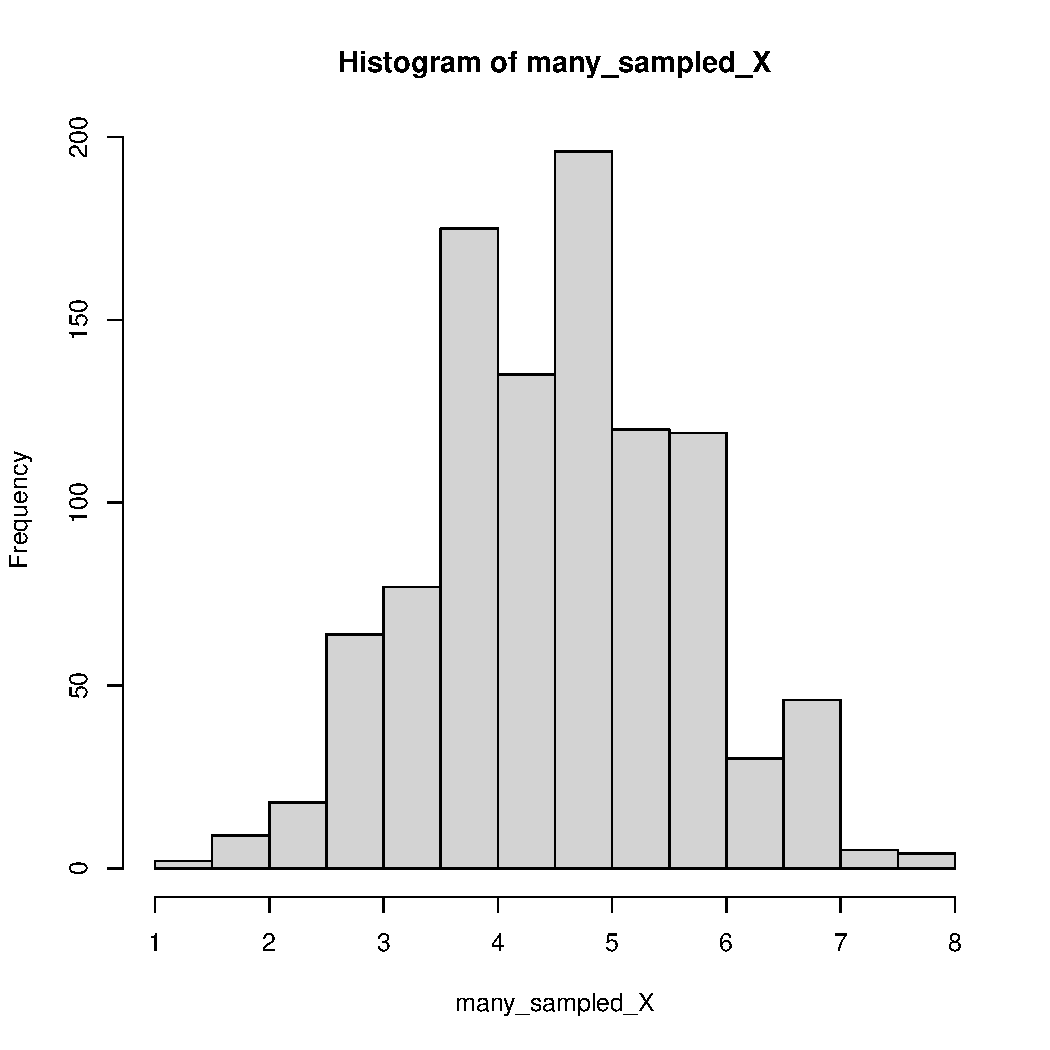
\includegraphics[width=\maxwidth]{images/statistics//unnamed-chunk-39-1} 
\begin{kframe}\begin{alltt}
\hldef{many_sampled_X}
\end{alltt}
\begin{verbatim}
##    [1] 4.2 6.8 7.4 5.0 3.8 6.0 5.8 6.0 4.0 2.8 3.2 3.2 4.0 4.0 4.4 3.8 4.4 5.4
##   [19] 4.6 5.8 4.4 4.4 5.2 6.4 5.8 4.0 5.8 4.0 3.6 4.0 3.0 2.2 5.4 4.8 4.0 2.4
##   [37] 7.6 4.6 4.2 4.0 6.8 2.8 5.4 3.2 4.0 2.8 4.8 5.2 4.2 6.4 5.0 4.4 3.2 3.8
##   [55] 4.4 4.0 5.2 4.0 5.0 3.8 5.8 3.2 7.0 4.0 2.8 4.0 5.2 4.2 6.6 4.4 5.2 5.4
##   [73] 3.0 6.0 4.4 4.6 3.6 3.6 4.4 6.8 3.0 4.8 4.4 3.8 4.8 5.6 4.2 5.4 5.4 4.6
##   [91] 5.0 4.6 3.8 4.4 5.0 6.0 2.0 4.0 4.6 5.0 3.8 3.8 3.6 4.8 5.2 7.0 3.8 5.0
##  [109] 3.6 3.8 5.8 3.8 5.0 3.4 4.0 4.4 4.4 3.4 2.6 6.6 3.8 4.4 5.8 4.0 4.0 4.0
##  [127] 6.0 4.0 2.2 4.0 4.2 4.6 4.2 3.2 4.8 4.8 3.8 2.2 5.6 3.2 4.8 4.6 4.4 4.8
##  [145] 3.8 4.6 5.0 4.6 4.2 5.4 4.0 3.4 1.4 6.0 5.2 1.4 6.0 4.8 3.6 4.4 3.6 5.8
##  [163] 4.6 3.4 5.6 5.0 5.0 6.0 4.2 4.0 4.2 4.8 5.6 5.8 3.6 5.0 5.4 4.8 4.0 5.4
##  [181] 4.0 5.8 6.4 3.6 3.6 4.8 4.0 3.4 4.6 6.0 4.4 5.0 6.4 3.4 4.0 4.6 4.4 5.2
##  [199] 2.2 2.8 5.6 5.4 3.2 5.6 4.6 3.4 3.4 5.0 4.2 4.2 5.8 4.4 5.4 4.8 5.6 6.8
##  [217] 2.2 5.2 6.6 3.2 6.2 4.2 4.2 4.0 4.2 2.8 5.2 4.6 4.8 6.2 3.6 4.4 4.8 4.4
##  [235] 5.4 6.0 4.2 3.6 4.8 5.6 3.4 4.8 3.8 5.2 4.8 5.0 3.8 5.2 3.2 4.2 4.0 5.2
##  [253] 2.2 2.6 5.0 4.6 4.0 4.4 4.8 3.0 5.2 7.6 4.0 5.2 4.8 6.2 3.2 5.4 2.8 5.4
##  [271] 4.8 4.8 4.0 5.6 2.6 4.2 5.0 3.0 4.0 6.4 5.2 3.2 3.6 4.6 4.2 6.4 5.4 7.0
##  [289] 4.6 4.2 4.8 6.2 4.4 4.8 4.2 3.6 3.2 5.4 5.8 4.4 3.4 6.8 4.6 6.0 3.6 6.0
##  [307] 4.6 3.0 5.4 3.8 3.4 4.4 3.0 4.2 3.8 6.0 3.8 4.2 4.0 4.2 4.4 5.8 3.6 5.2
##  [325] 4.0 2.6 6.8 3.2 3.4 5.2 3.8 4.2 4.4 3.2 2.8 4.6 3.8 4.6 6.4 1.8 4.4 4.6
##  [343] 5.2 2.4 3.4 5.2 4.8 5.8 5.0 5.6 5.2 3.4 7.0 4.2 5.0 6.6 5.6 3.4 3.2 5.8
##  [361] 3.6 4.6 3.6 5.2 5.2 3.6 3.4 6.2 3.8 4.6 3.4 4.8 5.2 5.0 2.8 3.6 4.2 5.6
##  [379] 5.4 5.4 4.0 5.2 3.4 3.8 3.6 3.8 5.2 6.6 3.8 6.2 4.6 5.2 3.0 4.8 2.8 2.8
##  [397] 4.8 5.2 4.2 5.0 5.2 4.8 6.2 5.4 6.0 5.0 3.8 6.6 5.6 3.8 3.6 3.4 3.6 5.6
##  [415] 6.2 3.2 3.8 3.2 6.8 5.0 4.2 4.6 4.2 4.6 5.8 4.0 5.0 6.8 3.8 3.6 5.2 2.4
##  [433] 4.4 4.4 3.6 5.2 6.6 3.8 6.0 5.8 5.4 3.6 5.2 4.0 4.8 2.8 5.0 4.6 6.0 4.8
##  [451] 4.4 3.8 4.8 4.4 3.0 4.0 6.2 4.4 4.6 5.0 5.6 3.8 3.2 4.0 4.4 4.4 6.6 4.0
##  [469] 5.6 3.8 2.4 5.4 4.2 3.4 4.0 6.0 5.0 2.6 5.4 5.0 4.4 5.2 4.8 5.6 4.0 4.2
##  [487] 4.6 5.6 4.4 4.0 4.8 5.0 6.0 3.8 7.2 2.2 3.4 2.8 5.4 4.4 5.2 6.4 4.2 6.4
##  [505] 5.4 4.0 5.0 3.6 5.4 4.2 4.2 6.8 1.6 2.6 3.2 4.4 6.0 4.6 5.2 7.6 4.4 3.0
##  [523] 4.8 2.0 4.2 4.6 4.8 5.6 6.0 4.4 4.0 4.2 2.6 6.2 4.8 4.0 3.2 5.8 4.4 5.2
##  [541] 2.6 5.0 4.4 4.2 5.0 4.6 4.4 4.2 3.8 6.0 6.2 6.0 5.0 5.4 6.0 4.0 3.6 2.0
##  [559] 6.0 5.4 5.2 4.2 4.2 4.8 3.8 4.2 3.4 4.2 3.0 3.4 2.6 4.4 4.6 3.8 4.6 5.0
##  [577] 3.4 3.8 3.6 4.0 4.0 4.8 3.4 4.8 5.0 3.2 3.6 3.8 4.6 6.2 6.6 4.6 3.4 4.6
##  [595] 5.8 3.8 4.2 5.2 5.8 5.2 4.8 4.8 3.2 5.4 3.8 3.6 6.8 4.0 5.4 5.6 5.8 5.2
##  [613] 5.4 5.8 5.0 2.2 4.0 3.6 5.0 5.8 6.8 4.6 4.4 4.6 3.6 5.8 3.8 5.4 5.2 5.2
##  [631] 3.6 5.6 4.6 5.2 3.8 2.2 6.6 6.0 6.6 4.2 3.2 5.0 5.4 5.4 5.2 6.8 5.0 4.2
##  [649] 7.2 5.2 4.2 4.4 6.8 4.0 6.8 5.6 4.8 5.4 4.8 6.8 2.8 4.8 3.4 5.0 3.2 4.0
##  [667] 5.0 5.4 4.2 4.2 6.2 5.4 4.0 2.4 3.6 4.0 5.6 3.6 2.8 5.0 5.0 5.2 5.0 6.8
##  [685] 4.0 3.6 4.8 4.6 4.4 5.4 4.4 3.6 6.0 3.8 5.4 3.4 3.0 5.6 3.8 5.6 3.2 4.8
##  [703] 6.0 5.6 6.0 4.4 2.6 6.8 7.0 5.0 4.6 4.8 3.4 3.6 3.0 4.6 5.2 4.2 5.0 5.6
##  [721] 5.4 5.6 3.6 6.8 4.6 6.0 4.4 6.0 5.4 4.4 4.0 4.6 2.8 3.4 5.2 4.6 3.8 2.6
##  [739] 2.8 3.2 4.6 4.6 6.6 6.0 4.6 3.0 4.2 2.8 3.8 5.4 6.2 6.8 2.0 2.6 4.8 3.4
##  [757] 5.4 4.0 5.2 6.0 4.4 6.2 3.0 5.8 6.8 5.6 3.6 4.6 4.2 6.0 4.6 4.6 3.4 2.2
##  [775] 5.4 6.0 4.8 3.4 6.0 4.8 4.4 4.2 5.0 4.6 3.0 7.0 7.0 3.6 4.8 4.0 3.4 5.8
##  [793] 5.4 3.0 2.8 4.4 4.0 5.8 4.8 4.2 3.4 5.0 5.2 3.8 4.6 2.0 6.2 5.2 5.2 4.8
##  [811] 5.2 4.6 4.0 2.6 5.8 3.2 4.4 4.8 4.6 5.4 3.0 5.6 2.2 3.2 5.4 2.8 5.4 6.2
##  [829] 5.8 5.0 5.6 3.4 3.4 3.6 4.6 4.6 5.2 4.8 4.0 4.4 5.0 5.2 5.6 3.0 6.0 3.2
##  [847] 2.6 2.8 4.0 4.4 5.8 4.0 4.0 5.2 7.2 7.2 4.4 3.6 2.8 5.0 4.0 5.6 4.6 4.4
##  [865] 3.2 5.8 4.6 5.8 5.0 4.6 2.8 4.2 2.2 5.2 4.6 4.4 4.0 2.0 5.4 4.0 6.0 4.8
##  [883] 3.6 6.2 4.4 5.6 3.8 4.2 4.8 4.2 4.2 5.4 4.4 5.2 7.8 6.0 2.0 5.0 2.6 6.2
##  [901] 3.8 4.0 5.0 4.8 5.4 5.6 4.8 3.0 4.2 5.2 5.2 4.4 5.0 6.0 4.6 5.4 4.6 6.4
##  [919] 5.6 3.4 5.2 4.2 4.0 5.8 4.4 3.6 3.2 5.4 5.0 3.2 4.6 4.4 5.8 6.2 5.4 5.8
##  [937] 7.0 3.8 5.2 3.2 5.2 5.2 6.0 4.6 5.4 7.0 4.0 5.6 3.0 5.8 4.8 3.0 5.6 3.0
##  [955] 4.0 4.2 2.6 4.2 4.2 3.2 4.8 4.2 7.0 4.0 7.0 6.6 3.6 3.4 5.0 5.6 4.8 4.8
##  [973] 4.6 3.4 4.6 3.0 3.6 4.4 4.4 4.2 4.0 3.2 6.0 4.8 3.8 5.6 5.2 6.8 4.6 4.2
##  [991] 5.6 6.6 6.0 3.4 4.6 2.8 3.8 2.2 4.4 4.6
\end{verbatim}
\end{kframe}
\end{knitrout}


\end{ExerciseList}


\section{Central Limit Theorem}

      \subsection{ The Standard Deviation}
      	The sample mean defined in Definition~\ref{d:sample_mean} gives us a notion of centrality of the sampled data which, if the data is sampled from the same distribution and it is independent, is an estimate of the mean of the distribution. We now define a concept which is the analogue for the standard deviation defined in Definition~\ref{d:standard_deviation}. Recall that for a distribution, the standard deviation measures of how the data distributes around its mean. 
      	\begin{definition}
      		\label{d:sampled_Standard_deviation}
      		\begin{equation}
      			\text{sd}(\underline X) =\sqrt{ \frac{ (X_1 - m(\underline X ))^2 + \ldots + (X_n - m(\underline X))^2)}{n-1}}
      		\end{equation}
      	\end{definition}
	Notice that the $\sqrt{}$ means that $\text{sd}(\underline X)$ has the same units and scales as $m(\underline X)$. The choice of dividing by $n-1$ rather than dividing by $n$ is of no importance for our scopes.

%<<Standard_Deviation>>=
%n <- 10000
%data = rnorm(n, mean = 3, sd = 3 )
%# Data from a gaussian distribution with standard deviation 3 
%sd(data)
%@

      \section{ Statement}
      
      In Subsection~\ref{ss:histogram} we have learned how histogram of independent samples rcan reconstruct the distribution. We can therefore have a better look at the distribution of the sample means by taking many samples 
      
\begin{knitrout}
\definecolor{shadecolor}{rgb}{0.969, 0.969, 0.969}\color{fgcolor}\begin{kframe}
\begin{alltt}
\hldef{n} \hlkwb{<-} \hlnum{1000}\hlcom{#sample_size }
\hldef{k} \hlkwb{<-} \hlnum{1000}\hlcom{#number of samples}
\hldef{Many_Sample_Means} \hlkwb{<-} \hlkwd{replicate}\hldef{(k,} \hlkwd{mean}\hldef{(}\hlkwd{sample}\hldef{(Moscow_heights, n )))}
\hlkwd{ggplot}\hldef{(} \hlkwc{data} \hldef{=} \hlkwd{tibble}\hldef{(}\hlkwc{x} \hldef{= Many_Sample_Means ))} \hlopt{+}
      \hlkwd{geom_histogram}\hldef{(} \hlkwd{aes}\hldef{( x ))} \hlopt{+}
      \hlkwd{geom_vline}\hldef{(} \hlkwc{xintercept} \hldef{=} \hlkwd{mean}\hldef{(Moscow_heights),} \hlkwc{col} \hldef{=} \hlsng{'red'}\hldef{)}
\end{alltt}


{\ttfamily\noindent\itshape\color{messagecolor}{\#\# `stat\_bin()` using `bins = 30`. Pick better value with `binwidth`.}}\end{kframe}
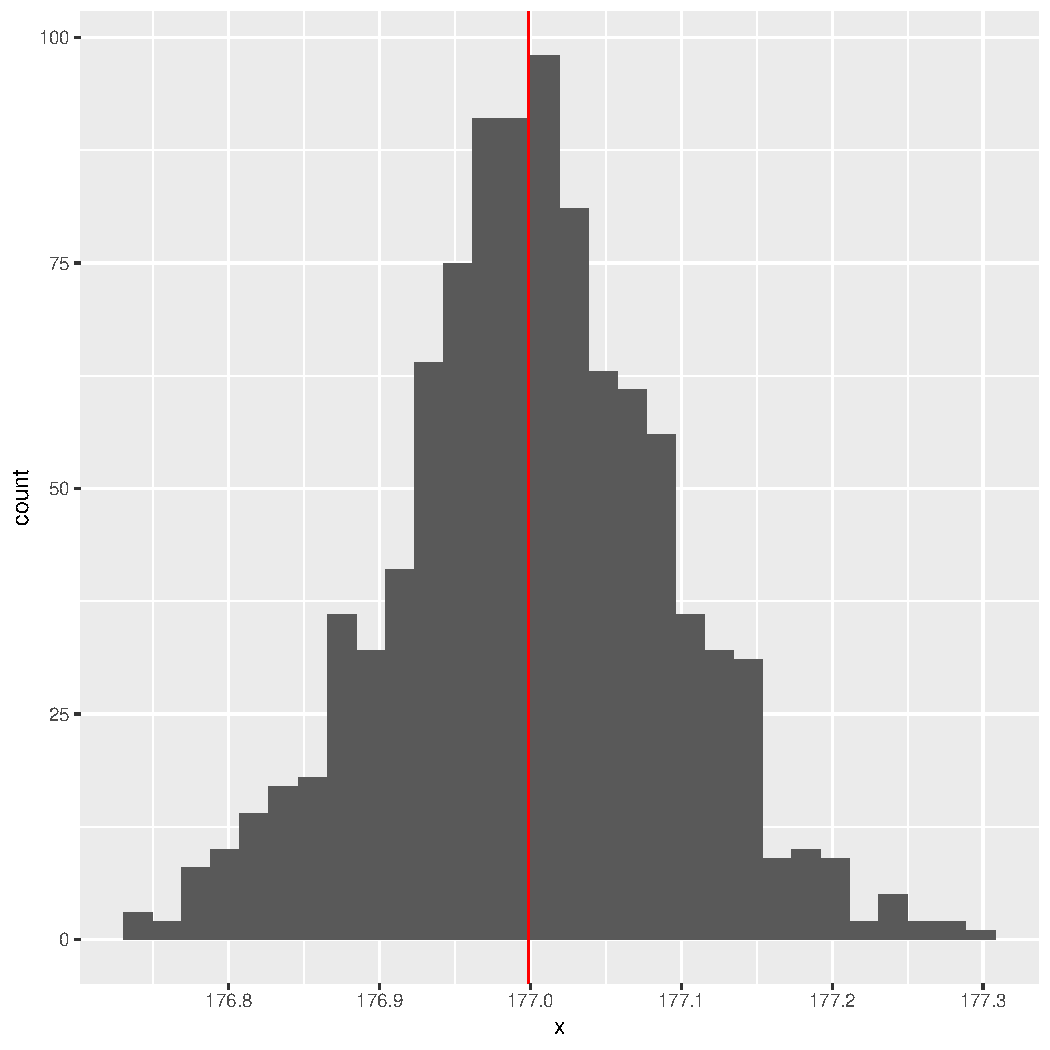
\includegraphics[width=\maxwidth]{images/statistics//unnamed-chunk-40-1} 
\end{knitrout}

      As expected from the Law of Large Numbers, the sample means concentrate around the real mean. The Central Limit Theorem answers to the quesiton of more precisely it ditributes around the mean. Analitically, the Law of Large Numbers tells us that
      \begin{equation}
	      \label{e:LLN1}
      	m_n(\underline X) = \frac{X_1 + \ldots + X_n}{n} = \mu + \text{Small Error}
      \end{equation}
      The Central Limit Theorem specifies furhter the structure of the small error: 
      \begin{equation}
      	\label{e:small_error}
      	\text{Small error } = \frac{\sigma}{\sqrt{n}} Z  + \frac{1}{\sqrt{n}} \textrm{Another small error}, 
      \end{equation}
      where $Z$ is a standard normal random variable.  Substituting \eqref{e:small_error} into \eqref{e:LLN1} we obtain 
      \begin{equation}
      	\frac{X_1 + \ldots + X_n}{n} = m(\underline X ) + \frac{\sigma }{\sqrt{n}}Z + \frac{1}{\sqrt{n}} \text{Another Small Error}
      \end{equation}
      Note that the $\sigma$ in \eqref{e:small_error} is necessary, since $Z$ does not have units of measure  (it is a universal object: its distribution is independent of the variables $X_i$!!! ). 
      Graphically, studying the quantity $\sqrt{n}\text{Small Error} = \sqrt{n} ( m(\underline X) - \mu)$ is the quantity that we obtain from the histogram of the sample means that we have plotted above if we center it and if we zoom in by a factor of $ \frac{\sqrt{n}}/\sigma$.( In an histogram, the data lies on the x axis and, therefore, zoomming in by a factor of $\sqrt{n}$ means that we dilatate the axis). We plot the density histogram since $Z$ is a continuous random variable   of density $\frac{1}{\sqrt{2\pi}}e^{-x^2/2}$. 
\begin{knitrout}
\definecolor{shadecolor}{rgb}{0.969, 0.969, 0.969}\color{fgcolor}\begin{kframe}
\begin{alltt}
\hldef{sample_size} \hlkwb{<-} \hlnum{10000}
\hldef{n_sample}  \hlkwb{<-} \hlnum{1000} \hlcom{# The number of sample means we look at to generate the histogram }
\hldef{Many_Samples}  \hlkwb{<-} \hlkwd{replicate}\hldef{(n_sample,} \hlkwd{mean}\hldef{(}\hlkwd{sample}\hldef{(Moscow_heights, sample_size )))}
\hldef{CLT} \hlkwb{<-}\hlkwd{sqrt}\hldef{(sample_size)}\hlopt{*}\hldef{( Many_Samples} \hlopt{-}   \hlkwd{mean}\hldef{(Moscow_heights))}\hlopt{/}\hlkwd{sd}\hldef{(Moscow_heights)}
\hlkwd{ggplot}\hldef{(} \hlkwc{data} \hldef{=} \hlkwd{tibble}\hldef{(}\hlkwc{x} \hldef{= CLT ))} \hlopt{+}
      \hlkwd{geom_histogram}\hldef{(} \hlkwd{aes}\hldef{(x,} \hlkwd{after_stat}\hldef{(density)),} \hlkwc{bins} \hldef{=} \hlnum{60}\hldef{)} \hlopt{+}
      \hlkwd{stat_function}\hldef{(} \hlkwc{fun} \hldef{=  dnorm,} \hlkwc{args} \hldef{=} \hlkwd{list}\hldef{(}\hlkwc{mean} \hldef{=} \hlnum{0}\hldef{,} \hlkwc{sd} \hldef{=} \hlnum{1} \hldef{),} \hlkwc{col} \hldef{=} \hlsng{'red'}\hldef{)}
\end{alltt}
\end{kframe}
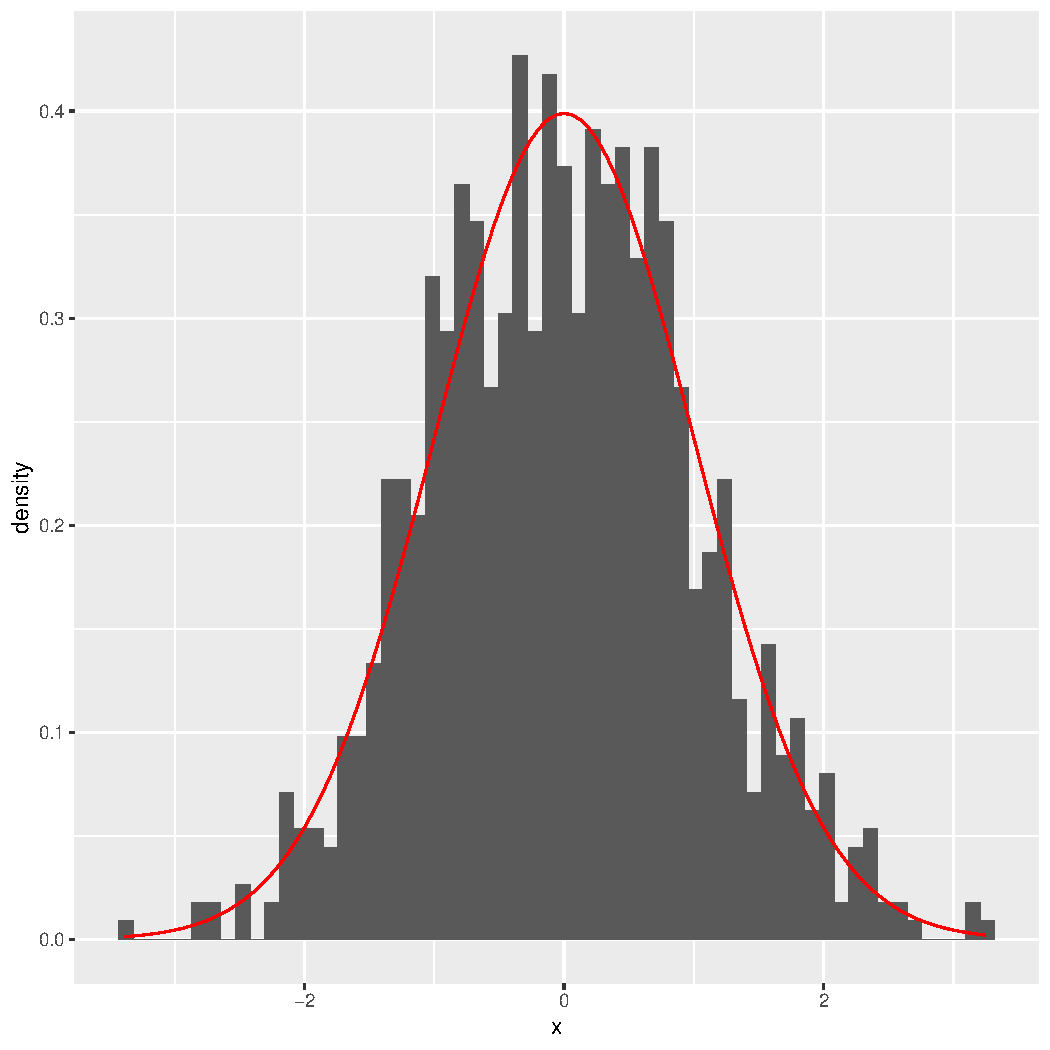
\includegraphics[width=\maxwidth]{images/statistics//unnamed-chunk-41-1} 
\end{knitrout}

      \begin{theorem}
      	\label{t:CLT}
      	Let $\underline X = ( X_1 , \ldots )$ be independent samples from a distribution that has a well defined mean $\mu$ and standard deviation $\sigma$. Then the distribution of 
      	\begin{equation}
      		\label{e:CLT1}
      		\sqrt{n}\frac{ m_n(\underline X) - \mu }{\sigma } 
      	\end{equation}
      	converges (in some sense ) to a standard Gaussian random variable $Z$  
      \end{theorem}
     In the case the sample comes from a population, the standard deviation of the random variable $X$ has to be substituted by the standard deviation of the population 
\begin{knitrout}
\definecolor{shadecolor}{rgb}{0.969, 0.969, 0.969}\color{fgcolor}\begin{kframe}
\begin{alltt}
\hlkwd{sd}\hldef{(Moscow_heights)}
\end{alltt}
\begin{verbatim}
## [1] 2.887133
\end{verbatim}
\end{kframe}
\end{knitrout}
Note that in contrast of the Law of Large Numbers, the random quantity \eqref{e:CLT1} converges to a random quantity $Z$. $Z$ depends, of course, from the sample $\underline X = (X_1, \ldots )$; however, its distribution does not. In this sense the Gaussians are a universal object and the Central Limit Theorem explains the fact that Gaussians are ubiquitous in science. Note that it is necessary to divide by $\sigma$, which has the same units of measure of the $X_i$, since the statement of the Central Limit Theorem guarantees that $Z$ does not have units of measure, since the quantity \eqref{e:CLT1}  has the same distribution in the limit for any unit of measure we use. 
   
      We finish this section by showing how does the quantity \eqref{e:CLT1} depend on the sample size $n$
\begin{knitrout}
\definecolor{shadecolor}{rgb}{0.969, 0.969, 0.969}\color{fgcolor}\begin{kframe}
\begin{alltt}
\hldef{Sample_size} \hlkwb{<-} \hlnum{100000}
\hldef{Sample} \hlkwb{<-} \hlkwd{rexp}\hldef{(Sample_size)}
\hlcom{# The exponential distribution  has standard deviation 1}
\hldef{sigma} \hlkwb{<-} \hlnum{1}
\hlcom{# and mean 1}
\hldef{mu} \hlkwb{<-} \hlnum{1}
\hldef{CLT} \hlkwb{<-} \hlkwd{sqrt}\hldef{((}\hlnum{1}\hlopt{:}\hldef{Sample_size))}\hlopt{*}\hldef{(} \hlkwd{cumsum}\hldef{(Sample)}\hlopt{/}\hlnum{1}\hlopt{:}\hldef{Sample_size} \hlopt{-} \hldef{mu)}\hlopt{/}\hldef{sigma}
\hlkwd{ggplot}\hldef{(} \hlkwc{data} \hldef{=} \hlkwd{tibble}\hldef{(}\hlkwc{x} \hldef{=} \hlnum{1}\hlopt{:}\hldef{Sample_size,} \hlkwc{y} \hldef{= CLT  ))} \hlopt{+}
        \hlkwd{geom_line}\hldef{(}\hlkwd{aes}\hldef{(x,y))}
\end{alltt}
\end{kframe}
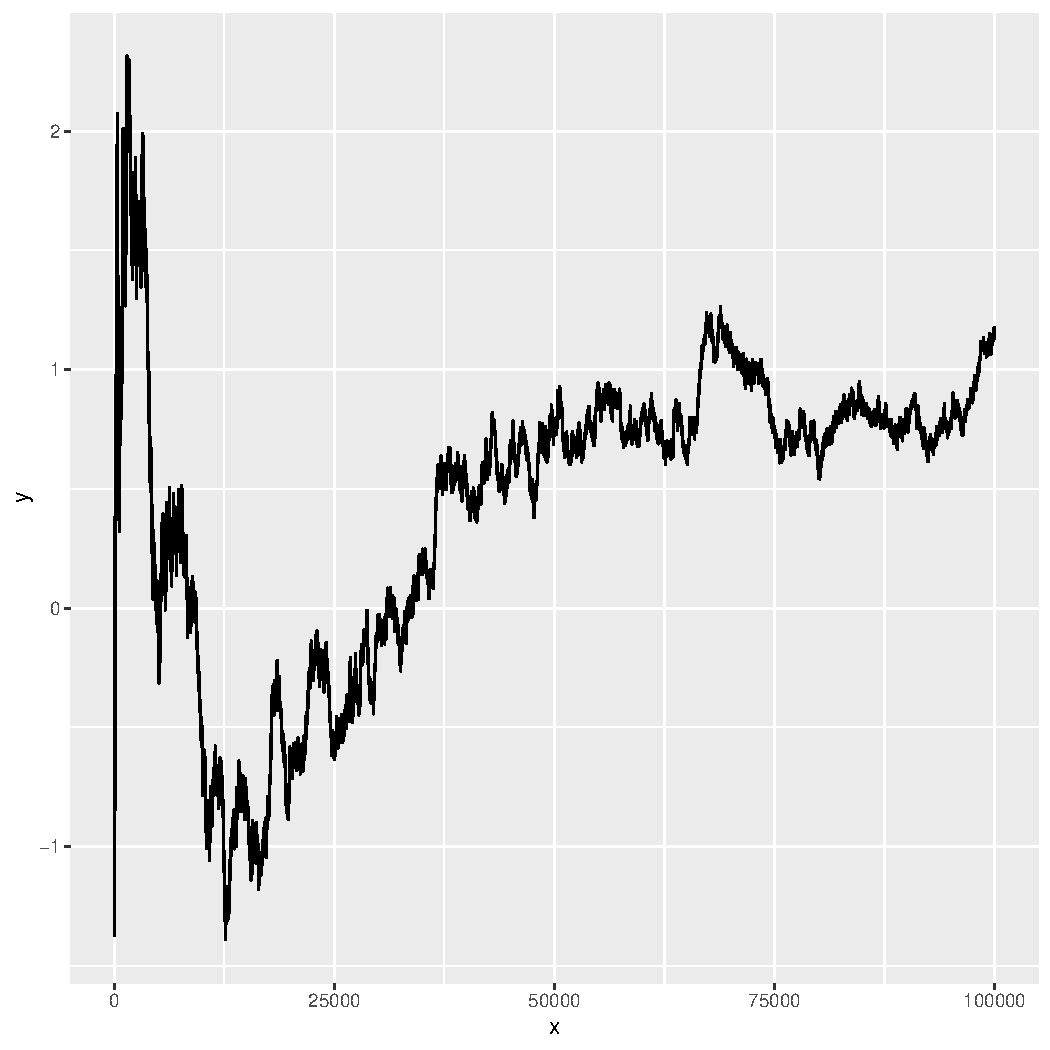
\includegraphics[width=\maxwidth]{images/statistics//unnamed-chunk-43-1} 
\end{knitrout}
as we can see from the graph, as soon as the sample size becomes big enough so that the Central Limit Theorem hold,  \eqref{e:CLT1} is a random quantity of order 1. 

      \begin{ExerciseList}
      	\Exercise Rewrite the codes of this Subsection and use it for samples from the exponential random variable, as in the example with the reaction times 
      \end{ExerciseList}

%      	\section{ Testing}
%      	
%      	A general framework for testing hypotheses is the following. We have data $\underline X = (X_1, \ldots, X_n)$ sampled from a variable and  established model,  the \emph{null hypothesis}, $H_0$ from which, provided it is valid, we know how the distribution with which the sample arises. We collect the data because we think that we should reject the null hypothesis in favour of the alternative models, collected in the \emph{alternative hypothesis} $H_1$. The picture we have in mind is summarised in Figure~\ref{f:}. We need to find a variable $t = t (\underline{X})$, function of the sample, that has two different behaviours whether $H_0$ true or $H_1$ are true. To fix the ideas, let's assume that $t$ tends to be greater if $H_1$ is true. Therefore, we wish to select a threshold $t_{\text{crit}}$ such that if $t(\underline X) >t_{\text{crit}}$ we reject $H_0$ in favour of $H_1$. The event $\{\underline X\, ,\, t(\underline X ) > t\} $ is drawn for two different values of $t$ in Figure~\ref{f:} and ~\ref{f:}. The above event can be true either in $H_0$, in which case we say that the statistics is big because of randomness, or from $H_1$, in which case we say that $t$ is big because of some real effect. To make a decision rule, we need to accept that due to randomness we can mistakenly reject $H_0$ in favour of $H_1$. 
%      	We fix a significance level $\alpha$, usually $\alpha = 0.05$ and we say that 
%      	\begin{definition}
%      		\label{d:p-value}
%      		The p-value associated to a statistic $t(\underline X)$ and to a null hypothesis $H_0$ is the probability to obtain a moreextremal statisic 
%      		\begin{equation}
%      			\label{e:p-value}
%      				\mathbb P( \{\underline X \, , \, t(\underline X ) > t_{\text{crit}}|H_0)
%      		\end{equation}
%      	\end{definition}
%      	Notice that more extremal is defined when defining the test. Since we are assuming that $t(\underline X)$ is greater under $H_1$, more extremal in this case means greater. In this case, the p-value associated to $t$. It 	ìis simply the survival function of the distribution of $t$ given $H_0$. It is easy to check that choosing $ t_{\text{crit} }$  such that $\mathbb $
%
%      	A very important point to make is that since the threshold $t_{\extrm{crit}}$ has been chosen disregarding $H_1$, even if the test rejects $H_0$ in favour of $H_1$, actually $\mathbb P(H_1|\underline X)$ can be small compared to $\mathbb P(H_0| \underline X)$, if the prior odds $\mathbb P(H_1)/\mathbb P(H_0)$ were small. Indeed
%      	\begin{equation}
%      		\label{e:odds_update}
%      			\frac{\mathbb P(H_1 | \underline X ) }{\mathbb P( H_0 | \underline X )} = \frac{\mathbb P( t > t_{\text{crit}} |H_1 ) }{\mathbb P( t > t_{\text{crit}}|H_0)}\frac{\mathbb P(H_1)}{\mathbb P(H_0)} < \alpha \frac{\mathbb P( H_1)}{\mathbb P(H_0)}
%      	\end{equation}
%      	where we have used the fact that $\mathbb P(\text{Rejected }|H_0) = \mathbb P( t > t_{\text{crit}}| H_0) \sim \alpha$ and that $\mathbb P(\text{" Test rejects $H_0$ "} | H_1 )  \leq 1$. As shown in Figure~\ref{f:}, the case in which the a priori. 
%      	This is the general framework for tests. A very interesting practical application, which shows wonderfully how difficult the estimations of the quantities $\frac{\mathbb P(H_1)}{\mathbb P(H_0)}$ and $\mathbb P(t > t_{\text{crit}})| H_1)$, which tests carefully avoid, are, can be found ate the links \url{} and \url{}.	
%      \subsection{ Testing interpretation of }
%
%
%      Recall from Section~\ref{s:binomial_test} that in that case $H_0:$ "The sample consists of independent observatiation and each informant uses the formal variant with probability $p = $" and $H_1:$ "The sample consists of independent observations and each informant uses the formal variant with probability $p >$". The statistics is $t = t( \underline{X}) = X_1 + \ldots + X_n$, where we are identifying formal with 1. We know the distribution of $t$ under $H_0$, a binomial of parameter $N$ and $p$, while under $H_1$ it is a binomial of a greater but unknown parameter. Therefore, values of $t$ that are big, bigger than $N ???$, give an hint  in favour of $H_1$. 
%
%      \subsection{ An example of a test }
      	
	
	If the samples are not independent but the 
      	\begin{ExerciseList}
      		\Exercise Think at an example where $X_i$ are all equally distributed but the Law of Large Numbers does not hold. ( Hint: what is the case in which the $X_i$ are most dependent? )
      	\end{ExerciseList}
      	
      	The scope of this subsection is to revisit the Eugene Onegin Example and put it in the jargon of testing. Apart from being interesting on its own, we see how to treat the case in which the distribution of the statistics is unknown also under $H_0$. Let $X_i$ denote if the i-th alphabet character is either a consonant, 1,  or a vowel, 0. The $X_i$ are all equally distributed as Bernoulli random variables and a good guess for the parameter $p$ is (we should take the russian drama corpus, but I want to avoid programming technicalitie s)
	\begin{itemize}
      		\item $H_0$: The $X_i$ follow a Bernoulli trial distribution ( see Definition~\ref{d:Bernoulli_trial}) and 
      		\item $H_1$: The $X_i$ form a Markov Chain: 
      			\begin{equation}
      				\label{}
      				\mathbb P()
      			\end{equation}
      			for some $q$ and $(1-q)$
      		\item The statistic that we use is $ s = \sqrt{n } ( m_n(\overline  ) - p)$, the one of the Central Limit Theorem 
      	\end{itemize}
      	It is very unlikely that the $H_1$ is true, but the point of testing is not to say whether $H_1$ is true but to refuse $H_0$ in favour of $H_1$. We can estimate $q_{01} =\mathbb P( X_{i+1} = 1 | X_i = 0)$ by counting the fraction of vowels followed by consonants, and  $q_{10} = \mathbb P( X_{i+1 } = 0 | X_i = 1)$ by counting the relative frequency of consonants followed by vowels.
<>>=



he Central Limit Theorem for the Bernoulli Trial Measure tells us that 
      \begin{equation}
      	\label{e:}
      \end{equation}
	

	\section{T-test} 
      	
	In this section we are going to introduce the z-test and the more conservative t-test, used to prove hypotheses concerning the mean of numerical variables. This section comes right after the Central Limit Theorem~\ref{t:CLT} since we will use it to approximate the distribution of the $t$ statistic, the quantity looked by both of these statistical tests, provided the null hypothesis holds. 

	\subsection{Standard Deviation }
	Recall that from a disribution of random variable we have defined the variance in Definition~\ref{d:variance} and the standard deviation in Definition~\ref{d:standard_deviation}. Similarly to what happens to the mean of the random variable $X$ and its sample mean associated to a sample$\underline X = (X_1, \ldots )$, see Definition~\ref{d:sample}, it is possible to define a sample standard deviation 
	\begin{definition}[Sampled standard deviation ]
		\label{d:sampled_sd}
		Let $\underline X = (X_1 , \ldots, X_n )$, be a vector of $n \in \mathbb N$ components, and recall the definition of (sample) mean of a vector in Definition~\ref{d:sample_mean}. The sampled standard deviation is 
		\begin{equation}
			\label{e:sampled_sd}
			\text{sd}_n(\underline X ) = \sqrt{\frac{(X_1 - m_n(\underline X ))^2 + \ldots  + (X_n - m_n(\underline X))^2}{n-1}}
		\end{equation}
	\end{definition}
	The fact that in the denominator there is the number $n-1$ instead of $n$ is due to statistical reasons that we do not study in the present notes. However, for $n$ large, the difference is minimal. 

	The same remarks as in the definition of standard deviation for a random variable in Definition~\ref{d:sd} apply. The sampled standard deviation has the same units of measure as the $X_i$ and it is a measure on how the data contained in the vector $\underline X$ distribute around the mean. If the $\underline X$ are independent samples from the same distribution, then the relation between the samples standard deviation $\text{sd}_n$ and the standard deviation of the distribution is the same one as the relation between the mean of the distribution $\mu$ and the sample mean $m_n$, se Definition~\ref{d:mean} and \ref{d:sample_mean}, and it is given by the Law of Large numbers 
      	\begin{proposition}
      		\label{d:standard_deviation}
		Let $\underline X = (X_1, \ldots )$ be a sample, see Definition~\ref{d:sample}, from a distribution of standard deviation $\sigma$.  
      		\begin{equation}
      			\label{e:standard_Deviation}
			\text{sd}_n(\underline X) \to \sigma
      		\end{equation}
		as $n\to \infty$
      	\end{proposition}
	Indeed, $ (X_1  - m_n(\underline X))^2,  (X_2 - m_n(\underline X))^2, \ldots$ are independent samples from the random variable $(X - \mu)^2$, where $\mu$ is the mean of the random variable $X$. The mean of $(X - \mu )^2$ is precisely $\text{Var}(X)$, see Definition~\ref{d:Variance} and, therefore, the Law of Large Numbers~\ref{t:LLN} implies that 
		\begin{equation}
			\frac{(X_1 - m_n(\underline X))^2 + \ldots + (X_n - m_n(\underline X))^2}{n} \to \text{Var}(X)
		\end{equation}
		
\begin{knitrout}
\definecolor{shadecolor}{rgb}{0.969, 0.969, 0.969}\color{fgcolor}\begin{kframe}
\begin{alltt}
\hldef{sample_size} \hlkwb{<-} \hlnum{1000}
\hldef{X} \hlkwb{<-} \hlkwd{rexp}\hldef{(sample_size)}
\hlkwd{sqrt}\hldef{(}\hlkwd{sum}\hldef{(X} \hlopt{-} \hlkwd{mean}\hldef{(X))}\hlopt{/}\hldef{(sample_size} \hlopt{-} \hlnum{1}\hldef{) )}
\end{alltt}
\begin{verbatim}
## [1] 9.399526e-09
\end{verbatim}
\begin{alltt}
\hlkwd{sd}\hldef{(X)}
\end{alltt}
\begin{verbatim}
## [1] 0.9617207
\end{verbatim}
\begin{alltt}
\hlcom{## The standard deviation of an exponential random variable is }
\end{alltt}
\end{kframe}
\end{knitrout}


	\begin{ExerciseList}
      		\Exercise Two samples $ \underline X$ and $\underline Y$ of two different numerical variables have been taken and the results visualized in  the histogram in Figure~\ref{f:hist}. Which one corresponds to a higher standard deviation? 
      	\end{ExerciseList}

      	\subsection{Intuition on the t-statistic}

      	The t-test is a test that is used for testing hypotheses on the mean of numerical variables. The example we will follow to introduce it in a practical level is the same one of the heights of the citizens of Moscow. We know that a good estimate for the heights of the citizens of Amsterdam is$\mu_{\text{Amsterdam}} = 178$, and we collect data to prove that the mean height of citizens of Moscow is inferior. To this end we take samples from the population of Moscow and test the following hypotheses
      	\begin{itemize}
      		\item $H_0$: The mean height of the citizens of Moscow is $\mu_{\text{Moscow}} = \mu_{\text{Amsterdam}}$ and we are taking independent samples 
      		\item $ H_1$: The mean height of the citizens of Moscow is $\mu_{\text{Moscow}}< \mu_{\text{Amsterdam}}$ and we are taking independent samples. 
      	\end{itemize}
      	Our aim is, once more, to give a rule to decide whether we have enough information to reject $H_0$ in favour of $H_1$. Of course all the discussions in Subsection~\ref{ss:Testing} hold and the proinciple of the t-test is no different from others
\begin{knitrout}
\definecolor{shadecolor}{rgb}{0.969, 0.969, 0.969}\color{fgcolor}\begin{kframe}
\begin{alltt}
\hldef{sample1} \hlkwb{<-} \hlkwd{c}\hldef{(}\hlnum{176}\hldef{,} \hlnum{178}\hldef{,} \hlnum{177}\hldef{,} \hlnum{175}\hldef{,} \hlnum{179}\hldef{)}
\end{alltt}
\end{kframe}
\end{knitrout}
oes the above sample give an hint in favour of $H_1$ with respect to $H_0$? Is the above sample sufficient to reject $H_0$ in favour of $H_1$? 
\begin{knitrout}
\definecolor{shadecolor}{rgb}{0.969, 0.969, 0.969}\color{fgcolor}\begin{kframe}
\begin{alltt}
\hldef{sample2} \hlkwb{<-} \hlkwd{c}\hldef{(}\hlnum{174}\hldef{,} \hlnum{176}\hldef{,} \hlnum{175}\hldef{,} \hlnum{173}\hldef{,} \hlnum{177}\hldef{)}
\end{alltt}
\end{kframe}
\end{knitrout}
      	Does the above sample give a stronger hint in favour of $H_1$ with respect to the first sample? If yes, why? The mean of \text{sample2???} is smaller than \text{sample1??}, and this is why it provides a stronger huint for $H_1$ tham the hint of sample1 
\begin{knitrout}
\definecolor{shadecolor}{rgb}{0.969, 0.969, 0.969}\color{fgcolor}\begin{kframe}
\begin{alltt}
\hldef{sample3} \hlkwb{<-} \hlkwd{c}\hldef{(}\hlnum{177}\hldef{,} \hlnum{177.5}\hldef{,} \hlnum{176.5}\hldef{,} \hlnum{178}\hldef{,} \hlnum{176}\hldef{)}
\end{alltt}
\end{kframe}
\end{knitrout}
      	Does the above sample give an hint in favour of $H_1$ with respect to $H_0$? Is the above sample sufficient to reject $H_0$ in favour of $H_1$?  Although \text{sample3??} has the same mean of \text{sample1????}, it provides a stronger int with respect to \text{sample1??} since there is 
\begin{knitrout}
\definecolor{shadecolor}{rgb}{0.969, 0.969, 0.969}\color{fgcolor}\begin{kframe}
\begin{alltt}
\hldef{sample4} \hlkwb{<-}    \hlkwd{c}\hldef{(}\hlnum{176}\hldef{,} \hlnum{178}\hldef{,} \hlnum{177}\hldef{,} \hlnum{175}\hldef{,} \hlnum{179}\hldef{,} \hlnum{176}\hldef{,} \hlnum{178}\hldef{,} \hlnum{177}\hldef{,} \hlnum{175}\hldef{,} \hlnum{179}\hldef{,} \hlnum{176}\hldef{,} \hlnum{178}\hldef{,} \hlnum{177}\hldef{,} \hlnum{175}\hldef{,} \hlnum{179}\hldef{,} \hlnum{176}\hldef{,} \hlnum{178}\hldef{,} \hlnum{177}\hldef{,} \hlnum{175}\hldef{,} \hlnum{179}\hldef{)}
\end{alltt}
\end{kframe}
\end{knitrout}
	
	All the above considerations are summarised in the \emph{t-statistic}
      \begin{definition}[t statistic]
      	\label{d:t-statistic}
      	Let $\underline X = (X_1,\ldots, X_n)$ be inedependent samples from a distribution, $\mu$ a guess for the mean of the distribution, $ m$ be the sample mean defined in \eqref{e:sample_mean} and $sd(\underline{X})$ the standard deviation defined in \eqref{e:sd}
      	\begin{equation}
      		\eqref{e:t_statistic}
      		t\equiv t_n(\underline{X},  \mu) = \sqrt{n}\frac{ m(\underline{X})  - \mu   }{\text{sd}(\underline{X})}
      	\end{equation}
      \end{definition}
      	We now compute the t-statistic of the above samples
\begin{knitrout}
\definecolor{shadecolor}{rgb}{0.969, 0.969, 0.969}\color{fgcolor}\begin{kframe}
\begin{alltt}
\hlcom{# The t-statistic is a function of the sample and of the hypotetic mean $\textbackslash{}mu$}
\hldef{t_stat} \hlkwb{<-} \hlkwa{function}\hldef{(} \hlkwc{X}\hldef{,} \hlkwc{mu}\hldef{) \{}
        \hlkwd{sqrt}\hldef{(n)}\hlopt{*}\hldef{(}\hlkwd{mean}\hldef{(X)} \hlopt{-} \hldef{mu)}\hlopt{/}\hlkwd{sd}\hldef{(X)}
\hldef{\}}
\end{alltt}
\end{kframe}
\end{knitrout}

If we assume that the null hypothesis $H_0$ holds, that is, that $\mu = 178 $ also for the Moscow population, we can compute the associated t-statistic 

\begin{knitrout}
\definecolor{shadecolor}{rgb}{0.969, 0.969, 0.969}\color{fgcolor}\begin{kframe}
\begin{alltt}
\hlkwd{t_stat}( sample1, 178) 
\hlkwd{t_stat}(sample2, 178) 
\hlkwd{t_stat}(sample3, 178)
\hlkwd{t_stat}(sample4. 178)
\end{alltt}


{\ttfamily\noindent\bfseries\color{errorcolor}{\#\# Error in parse(text = input): <text>:4:17: costante numerica inattesa\\\#\# 3: t\_stat(sample3, 178)\\\#\# 4: t\_stat(sample4. 178\\\#\# \ \ \ \ \ \ \ \ \ \ \ \ \ \ \ \ \ \ \ \textasciicircum{}}}\end{kframe}
\end{knitrout}

As we can see, the t-statistic of \textrm{sample2}, \textrm{sample3}  and \textrm{sample4} is smaller than the one obtained for \textrm{sample4}. The reason is that \eqref{e:t-statistic} contains the expressions that en $m_5(\textrm{sample2}) < m\textrm{sample1})$, in the first case, in the second case $\text{sd}_5 (\textrm{sample3}) <\text{sd}_5 (\textrm{sample3})$, in the second case, and in the last case the t-statistic is smaller since $n$  is much bigger for \textrm{sample4}.   
Both the t-test and the z-test use the t-statistic, and the decision rule is, assuming that under $H_1$ a smaller $t$ is more probable, is to reject $H_0$ in favour of $H_1$ if $t < t_{\text{crit}}$ for a certain $ t_{\text{crit}}$. How $t_{\text{crit}}$ is decided defined the test
      Placing the above considerations in the framework for testing hypotheses described in Subsection~\ref{ss:hypotheses_testing}, we have 
      
      \begin{itemize}
		\item A null 
		\item An alternative hypotheses
		\item A notion of estremality, 
	\end{itemize}
	The decision


      \subsection{Z-test}
      If $H_0$ is true, then the expression \eqref{e:t_statistic} resambles the expression \eqref{e:CLT} in the Central Limit Theorem, with the only difference that the standard deviation is substituted by the sample standard deciation. However, the Law of Large Numbers tells that these two quantites coincide. If the sample size $n$ is big enough, then the Central Limit Theorem guarantees that under $H_0$ the t-statistic follows a standard normal distribution. 

nowing (approximately) the distribution of $t$ allows us to define a $t_{\text{crit}}$ in the usual way. We fix an $\alpha  >0$, usually $\alpha = 0.5$ and we choose $t_{\text{crit}}$ such that the probability of making a type 1 error, provided $H_0$ holds, is $\alpha$. Since 
      \begin{equation}
      	\label{e:t_crit}
      		\mathbb P(\text{"$H_0$ rejected "}|H_0) = \mathbb P( t < t_{\text{crit}}| H_0 ) \sim \frac{1}{\sqrt{2\pi}}\int_{-\infty }^{t_{\text{crit}}} e^{-\frac{x^2}{2}}dx
      \end{equation}
      and the above quantity has to be equal to 
      Graphically we are looking for the biggest $t_{\text{crit}}$ so that the mass on its left is smaller than $\alpha$, which is sometimes called the left inverse of the cumulative distribution function and is already implemented in R 

      Equivalently, we reject $H_0$ if and only if the p-value of the statistics observed is smaller than $\alpha$. To this end. 
      The Z-test is already implementedi 
      	
      \section{T-test}

      If the $X_i$ are sampled from a Guassian distribution of mean $\mu$, then the $t$-statistics associated to $\mu$ and $n$ follows a t-student distribution with $n$ degrees of freedom 
\begin{knitrout}
\definecolor{shadecolor}{rgb}{0.969, 0.969, 0.969}\color{fgcolor}\begin{kframe}
\begin{alltt}
	function \hlkwd{t_statistic}(x, mu, ) \{
    	  \hlkwd{return} ( \hlkwd{sqrt}(\hlkwd{length}(x))*( \hlkwd{mean}(x ) - mu)/\hlkwd{sd}(x))

sample_size <- 5
n <- 10000
data <- \hlkwd{replicate}(k, \hlkwd{t_statistic}(\hlkwd{rnorm}(sample_size, mean = mu_h0, sd = 1))
\hlkwd{gplot}(data = \hlkwd{tibble}( x= t_statistic))  + 
      \hlkwd{geom_histogram}( \hlkwd{aes}(x , y = \hlkwd{after_stats}(density)) + 
      	       \hlkwd{geom_line}(data = \hlkwd{tibble}(x = -7:7, y = \hlkwd{stsudent}(-7:7), args = \hlkwd{list}(df = n-1))\hlkwd{aes}(x = 1:k , y = ))
\end{alltt}


{\ttfamily\noindent\bfseries\color{errorcolor}{\#\# Error in parse(text = input): <text>:1:18: simbolo inatteso\\\#\# 1: \ \ \ \ \ \ \ \ function t\_statistic\\\#\# \ \ \ \ \ \ \ \ \ \ \ \ \ \ \ \ \ \ \ \ \ \textasciicircum{}}}\end{kframe}
\end{knitrout}
The t-test is defined by assuming that . Since the tails of the t-student distribution weight more than the ones of the normal, we have that the critical $t$ of the t-test is greater that the one for the Z-test. In other terms is more conservative. 
\begin{knitrout}
\definecolor{shadecolor}{rgb}{0.969, 0.969, 0.969}\color{fgcolor}\begin{kframe}
\begin{alltt}
\hldef{alpha} \hlkwb{=} \hlnum{0.095}
\hldef{n} \hlkwb{=} \hlnum{10}
\hlkwd{qtstudent}\hldef{(} \hlkwc{df} \hldef{= n}\hlopt{-} \hlnum{1}\hldef{)}
\end{alltt}


{\ttfamily\noindent\bfseries\color{errorcolor}{\#\# Error in qtstudent(df = n - 1): non trovo la funzione "{}qtstudent"{}}}\begin{alltt}
\hlkwd{t.test}\hldef{()}
\end{alltt}


{\ttfamily\noindent\bfseries\color{errorcolor}{\#\# Error in t.test.default(): argomento "{}x"{} assente, senza valore predefinito}}\end{kframe}
\end{knitrout}
	\subsection{t-test}

	The t-test differs from the z-test only by the fact that the distribution of $t= t_n(\underline X)$, provided $H_0$ holds, is assumed  to be a t-student distribution of $n-1$ degrees of freedom. This gives rise to different p-values and to a different $t_{\text{crit}}$. 
	For each $x$, if we observe the event $X = x$ the distribution of $Y$ changes (unless $X$ and $Y$ are independent, see Definition~\ref{d:independent}). We denote by $\mu(x)$ the mean of $Y$ given $X$.

\begin{knitrout}
\definecolor{shadecolor}{rgb}{0.969, 0.969, 0.969}\color{fgcolor}\begin{kframe}
\begin{alltt}
\hldef{plot_regression} \hlkwb{<-} \hlkwa{function}\hldef{(}\hlkwc{x}\hldef{,} \hlkwc{y}\hldef{,} \hlkwc{m_guess}\hldef{,} \hlkwc{b_guess}\hldef{) \{}
  \hldef{data} \hlkwb{<-} \hlkwd{data.frame}\hldef{(x, y)}

  \hlcom{# Compute guessed line}
  \hldef{y_guess} \hlkwb{<-} \hldef{m_guess} \hlopt{*} \hldef{x} \hlopt{+} \hldef{b_guess}
  \hldef{residuals} \hlkwb{<-} \hldef{y} \hlopt{-} \hldef{y_guess}
  \hldef{data}\hlopt{$}\hldef{y_guess} \hlkwb{<-} \hldef{y_guess}
  \hldef{data}\hlopt{$}\hldef{residuals} \hlkwb{<-} \hldef{residuals}

  \hlcom{# Base plot with points}
  \hldef{plot} \hlkwb{<-} \hlkwd{ggplot}\hldef{(data,} \hlkwd{aes}\hldef{(}\hlkwc{x} \hldef{= x,} \hlkwc{y} \hldef{= y))} \hlopt{+}
    \hlkwd{geom_point}\hldef{(}\hlkwc{color} \hldef{=} \hlsng{'blue'}\hldef{,} \hlkwc{size} \hldef{=} \hlnum{3}\hldef{)} \hlopt{+}
    \hlkwd{geom_abline}\hldef{(}\hlkwc{intercept} \hldef{= b_guess,} \hlkwc{slope} \hldef{= m_guess,} \hlkwc{color} \hldef{=} \hlsng{'red'}\hldef{,} \hlkwc{linetype} \hldef{=} \hlsng{'solid'}\hldef{,} \hlkwc{size} \hldef{=} \hlnum{1}\hldef{)} \hlopt{+}
    \hlkwd{labs}\hldef{(}\hlkwc{title} \hldef{=} \hlsng{'Linear Regression Guess with Residuals'}\hldef{,} \hlkwc{x} \hldef{=} \hlsng{'X'}\hldef{,} \hlkwc{y} \hldef{=} \hlsng{'Y'}\hldef{)} \hlopt{+}
    \hlkwd{theme_minimal}\hldef{()}

  \hlcom{# Add residual lines and labels}
  \hldef{plot} \hlkwb{<-} \hldef{plot} \hlopt{+} \hlkwd{geom_segment}\hldef{(}\hlkwd{aes}\hldef{(}\hlkwc{x} \hldef{= x,} \hlkwc{y} \hldef{= y,} \hlkwc{xend} \hldef{= x,} \hlkwc{yend} \hldef{= y_guess),} \hlkwc{color} \hldef{=} \hlsng{'green'}\hldef{)} \hlopt{+}
    \hlkwd{geom_text}\hldef{(}\hlkwd{aes}\hldef{(}\hlkwc{label} \hldef{=} \hlkwd{round}\hldef{(residuals,} \hlnum{2}\hldef{),} \hlkwc{y} \hldef{= (y} \hlopt{+} \hldef{y_guess)} \hlopt{/} \hlnum{2}\hldef{),} \hlkwc{color} \hldef{=} \hlsng{'green'}\hldef{,} \hlkwc{hjust} \hldef{=} \hlopt{-}\hlnum{0.3}\hldef{,} \hlkwc{size} \hldef{=} \hlnum{3}\hldef{)}

  \hlkwd{print}\hldef{(plot)}
\hldef{\}}

\hlcom{# Example Data}
\hldef{x} \hlkwb{<-} \hlkwd{c}\hldef{(}\hlnum{1}\hldef{,} \hlnum{2}\hldef{,} \hlnum{3}\hldef{,} \hlnum{4}\hldef{,} \hlnum{5}\hldef{)}
\hldef{y} \hlkwb{<-} \hldef{x} \hlopt{+} \hlkwd{rnorm}\hldef{(}\hlnum{5}\hldef{)}

\hlcom{# Example Guess (wrong on purpose)}
\hldef{m_guess} \hlkwb{<-} \hlnum{1.8}  \hlcom{# Slope guess}
\hldef{b_guess} \hlkwb{<-} \hlnum{0.5}  \hlcom{# Intercept guess}

\hlkwd{plot_regression}\hldef{(x, y, m_guess, b_guess)}
\end{alltt}


{\ttfamily\noindent\color{warningcolor}{\#\# Warning: Using `size` aesthetic for lines was deprecated in ggplot2 3.4.0.\\\#\# i Please use `linewidth` instead.\\\#\# This warning is displayed once every 8 hours.\\\#\# Call `lifecycle::last\_lifecycle\_warnings()` to see where this warning was generated.}}\end{kframe}
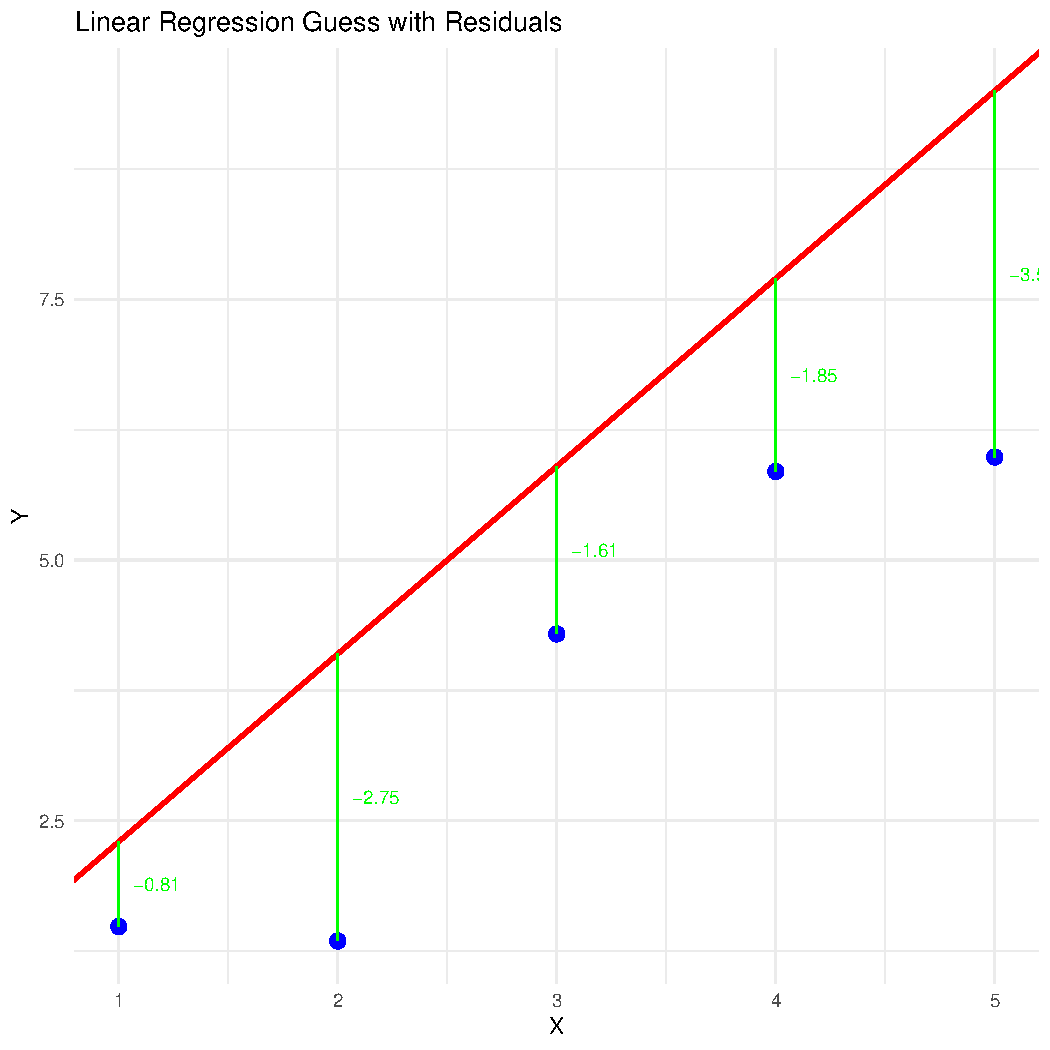
\includegraphics[width=\maxwidth]{images/statistics//unnamed-chunk-48-1} 
\end{knitrout}

	
	\subsection{ Sample mean as a minimum}
	
	\bel{e:sample_mean1}{
		\mathbb E[( X- \mu)^2]\sim \sum_{i = 1}^n ( X_i - \mu )^2 
	}
	and, quite surprisigly, this $\sim$ property commutes with the $\min_{\mu}$ operator!. (It is not really surprising since the probability on the right hand side is made by taking the sample mean )
	Therefore, if 
	\subsection{ Mean as a predictor}
	
		The linear regression assumes you want to predict the value of $Y$ using its mean. If there is no $X$ variable re 
	\section{Some precautions to take when testing}
	\subsection{Perform tests after looking at the data }

	\subsection{Multiple Comparisons}

	Another similar issue happens when performing multiple tests. As an example, think of correcting an exam which  has a cartain number of questions, say 30, at an high school. To decide whether or not two different students have cheated, we perform a simple test and decide that two students have copied from each other if the $k = k(\alpha)$  out of 30 answer coincide (here $k$ depends on the significance level we want. The smaller the $\alpha$, the closer the $k$ to 30). Now, in the classroom there are 20 students sitting next to each others in pairs, and we decide only to test those pairs since they are most at risk of copying. \\
	The underlying assumption is that the null hypothesis $H_0$ comes with a model for the possible outcomes of two exams that where made by students that did not copy for each other, so that, under $H_0$, we can compute 
	\bel{}{
		\mathbb P( \#  > k )
	}
	and define $k = k(\alpha)$, the critical value for which without copying, whose precise form is not important for illustrating the multiple comparison problem, that allows us to compute As usual, $k(\alpha$) is de 
	As a practical example, the correlation from a le
	
	\subsection{ }
	Given $Y$ 
	Assume we observe a sample $\underline Y = (Y_1, \ldots, Y_n)$ of sample size $n \in \mathbb N$ from a random variable $Y$. We want to use the previous information to make a more informed prediction for $Y$. It is possible to  
      
	\subsection{ Multivariate Regression} 
		It is straghtforward to extend the previous framework to the multivariate in which for each observation we collect more than two numerical variables. To fix the ideas, let us consider three variables, $X$ $Y$ and $Z$, and let $\underline X = (X_1, \ldots, X_n)$, $\underline Y =(Y_1, \ldots, Y_n)$ and $\underline Z = (Z_1, \ldots, Z_n)$ be samples of size $n \in \mathbb N$. Using the sample, which is a random quantity, we want to estimate the deterministic quantity   
	\bel{}{
		\mathbb E\left[ Z | X,Y \right]
	}
	which is a function of the possible values $X$ and $Y$ might assume. To this end we use the characterization \eqref{e:minimum}
	\bel{eq:minimum}{
		\mathbb E\left[ (Z - \mathbb E[ Z |X,Y])^2|X,Y\right] = \min_{\mu(x,y) } \mathbb E\left[ (Z - \mu(X,Y))\right|X,Y]^2
	} 
	so that we choose $\hat Z$ so as to minimize the above quantity. This is the real $\hat Z$. How to estimate the fake one???
	\bel{}{
		\hat Z =
	}
	\url{https://www.tylervigen.com/spurious/correlation/4018_american-cheese-consumption_correlates-with_blackrocks-stock-price}
	\section{Some other interesting references}

An article that I haven't read of linear regression in Linguistic Data: \url{https://pmc.ncbi.nlm.nih.gov/articles/PMC5911484/}
A very good answer to the question (if you ever had it) to why p-values that are too small are not reported \url{https://stats.stackexchange.com/questions/78839/how-should-tiny-p-values-be-reported-and-why-does-r-put-a-minimum-on-2-22e-1}
Another book on line
	\subsection{ Eugene Onegin}
	\label{ss:Eugene_Onegin4}
	We now continue and conclude Example~\ref{ex:Eugene_Onegin1}, \ref{ex:Eugene_Onegin2} and \ref{ex:Eugene_Onegin3}. 
Recall that from a text in russian we have defined a sequence $\underline X$ whose ith digit $X_i$ can be 0, indicating that in the i-th place there is a vowel, or 1, indicating a consonant.
%<<>>= 
%ger <- rdracor::get_dracor(corpus = 'ger')
%binary_transform_ger <- function(drama_name){
%  text <- rdracor::get_text_chr_spoken(play = drama_name, corpus = "ger")
%  all_text <- paste(text, collapse = "")
%  letters_vector <- tolower(unlist(strsplit(all_text, "")))
%  spoken_chars <- c(
%    letters,         # a–z
%    "ä", "ö", "ü",   # umlauts
%    "ß"              # sharp S (Eszett)
%  )
%  filtered_letters_vector <- letters_vector[ letters_vector %in% spoken_chars]  # Keep only Russian letters
%  german_vowels <- c("a", "e", "i", "o", "u", "ä", "ö", "ü")
%  binary_sequence <- ifelse(filtered_letters_vector %in% german_vowels, 0, 1)
%  return(binary_sequence)
%}
%
%vec <- vector(mode = 'numeric')
%for( play_name in ger$playName){
%  vec <- c(vec, binary_transform_ger(play_name))
%}
%@
%
% Intuitively, the digits of this sequence are not independent and, if we observe many consecutive 1s, it is more likely to find a 0, since otherwise the corresponding word would be difficult to pronounce. In Example~\ref{ex:Eugene_Onegin1} we have introduced two models
	\begin{itemize}
		\item $H_0$: $\underline X$ is an instance of a Bernoulli trial measure $\mathbb P_p$ for some $p \in [0,1]$, see Definition~\ref{d:Bernoulli}.
		\item $H_1$: $\underline X$ is an instance of the two-state Markov model $\mathbb P_{a,b}$ for some $a,b \in [0,1]$, see Definition~\ref{d:Markov}   
	\end{itemize}
	For the sake of readibility, we recall the two aforementioned distributions. For $x_1, \ldots, x_n \in\{0,1\}$ a fixed sequence of digits belonging to 0 and 1, with $n \in \mathbb N$, the model $H_0$ assumes   
	\bel{}{
		\mathbb P_p(X_1 = x_1, \ldots, X_n = x_n) = \prod_{i = 1  }^n \mathbb P_p( X_i = x_i) = p^{x_1 + ... + x_n }(1- p )^{n - (x_1 + \ldots + x_n)}
	}
	and the model $H_1$ assumes 
	\bel{}{
		\mathbb P_{a,b}( X_1 = x_1 , \ldots, X_n = x_n) & = \mathbb P_{a,b}( X_1 = x_1 ) \mathbb P_{a,b}(X_2 = x_2 | X_1 = x_1) \ldots \mathbb P_{a,b}(X_n = x_n |X_{n-1} = x_{n-1}) \\
		& = \mathbb P(X_1 = x_1) \prod_{ i = 1 }^n P_{x_{i-1}, x_{i}}
	}	
	where the \emph{transition matrix} $P(x, y)$, whose meaning is precisely $\mathbb P(X_{i + 1}= y | X_i = x ) = P_{x,y}$ for every $i \in\mathbb N$, is given by the following values 
	\bel{}{
		P_{0,0} = (1-a), \quad P_{01} = a, \quad P_{1,0} = b, \quad, P_{1,1} = 1-b
	}
	Recall also that in Example~\ref{ex:Eugene_Onegin} we have estimated the parameter $p$ for the first model, and the parameters $a$ and $b$ for the second model
\begin{knitrout}
\definecolor{shadecolor}{rgb}{0.969, 0.969, 0.969}\color{fgcolor}\begin{kframe}
\begin{alltt}
\hldef{from} \hlkwb{<-} \hldef{vec[}\hlopt{-}\hlkwd{length}\hldef{(vec)]}
\end{alltt}


{\ttfamily\noindent\bfseries\color{errorcolor}{\#\# Error: oggetto 'vec' non trovato}}\begin{alltt}
\hldef{to} \hlkwb{<-} \hldef{vec[}\hlopt{-}\hlnum{1}\hldef{]}
\end{alltt}


{\ttfamily\noindent\bfseries\color{errorcolor}{\#\# Error: oggetto 'vec' non trovato}}\begin{alltt}
\hlcom{# Count transitions}
\hldef{n_01} \hlkwb{<-} \hlkwd{sum}\hldef{(from} \hlopt{==} \hlnum{0} \hlopt{&} \hldef{to} \hlopt{==} \hlnum{1}\hldef{)}
\end{alltt}


{\ttfamily\noindent\bfseries\color{errorcolor}{\#\# Error: oggetto 'from' non trovato}}\begin{alltt}
\hldef{n_00} \hlkwb{<-} \hlkwd{sum}\hldef{(from} \hlopt{==} \hlnum{0} \hlopt{&} \hldef{to} \hlopt{==} \hlnum{0}\hldef{)}
\end{alltt}


{\ttfamily\noindent\bfseries\color{errorcolor}{\#\# Error: oggetto 'from' non trovato}}\begin{alltt}
\hldef{n_10} \hlkwb{<-} \hlkwd{sum}\hldef{(from} \hlopt{==} \hlnum{1} \hlopt{&} \hldef{to} \hlopt{==} \hlnum{0}\hldef{)}
\end{alltt}


{\ttfamily\noindent\bfseries\color{errorcolor}{\#\# Error: oggetto 'from' non trovato}}\begin{alltt}
\hldef{n_11} \hlkwb{<-} \hlkwd{sum}\hldef{(from} \hlopt{==} \hlnum{1} \hlopt{&} \hldef{to} \hlopt{==} \hlnum{1}\hldef{)}
\end{alltt}


{\ttfamily\noindent\bfseries\color{errorcolor}{\#\# Error: oggetto 'from' non trovato}}\begin{alltt}
\hlcom{# We estimate the jump probability from 0 to 1 }
\hlcom{# n_00 + n_01 is the total number of jumps from 0, i.e., the total number of 0 }
\hldef{a_hat} \hlkwb{<-} \hldef{n_01} \hlopt{/} \hldef{(n_00} \hlopt{+} \hldef{n_01)}  \hlcom{# P(1 | 0)}
\end{alltt}


{\ttfamily\noindent\bfseries\color{errorcolor}{\#\# Error: oggetto 'n\_01' non trovato}}\begin{alltt}
\hlcom{# We estimate the jump probability from 1 to 0 }
\hldef{b_hat} \hlkwb{<-} \hldef{n_10} \hlopt{/} \hldef{(n_10} \hlopt{+} \hldef{n_11)}  \hlcom{# P(0 | 1)}
\end{alltt}


{\ttfamily\noindent\bfseries\color{errorcolor}{\#\# Error: oggetto 'n\_10' non trovato}}\begin{alltt}
\hldef{p_1} \hlkwb{<-} \hldef{(n_10} \hlopt{+} \hldef{n_11)} \hlopt{/} \hldef{(n_00} \hlopt{+} \hldef{n_01} \hlopt{+} \hldef{n_10} \hlopt{+} \hldef{n_11)}
\end{alltt}


{\ttfamily\noindent\bfseries\color{errorcolor}{\#\# Error: oggetto 'n\_10' non trovato}}\begin{alltt}
\hldef{p} \hlkwb{<-} \hlkwd{mean}\hldef{(vec)}
\end{alltt}


{\ttfamily\noindent\bfseries\color{errorcolor}{\#\# Error in mean(vec): oggetto 'vec' non trovato}}\begin{alltt}
\hlcom{# Print estimated transition matrix}
\hlkwd{cat}\hldef{(}\hlsng{"Estimated transition matrix:\textbackslash{}n"}\hldef{)}
\end{alltt}
\begin{verbatim}
## Estimated transition matrix:
\end{verbatim}
\begin{alltt}
\hlkwd{print}\hldef{(}\hlkwd{matrix}\hldef{(}\hlkwd{c}\hldef{(}\hlnum{1} \hlopt{-} \hldef{a_hat, a_hat, b_hat,} \hlnum{1} \hlopt{-} \hldef{b_hat),} \hlkwc{nrow} \hldef{=} \hlnum{2}\hldef{,} \hlkwc{byrow} \hldef{=} \hlnum{TRUE}\hldef{,}
             \hlkwc{dimnames} \hldef{=} \hlkwd{list}\hldef{(}\hlkwc{from} \hldef{=} \hlkwd{c}\hldef{(}\hlsng{"0"}\hldef{,} \hlsng{"1"}\hldef{),} \hlkwc{to} \hldef{=} \hlkwd{c}\hldef{(}\hlsng{"0"}\hldef{,} \hlsng{"1"}\hldef{))))}
\end{alltt}


{\ttfamily\noindent\bfseries\color{errorcolor}{\#\# Error in matrix(c(1 - a\_hat, a\_hat, b\_hat, 1 - b\_hat), nrow = 2, byrow = TRUE, : oggetto 'a\_hat' non trovato}}\end{kframe}
\end{knitrout}
	We have already seen th

	and that we have defined the statistic of the jumps between 0s and 1s to see that it differs significantly from the one of the Bernoulli model $H_0$, see \eqref{}. 
	In this last part of the example we compute the statistic that Markov originally computed in his paper \cite{Markov} using the Eugene Onegin poem.   \\
	The Central Limit Theorem~\ref{t:CLT} states that the fluctuations from the mean of i.i.d. random variables $X_1, \ldots, X_n$ with finite variance, that is, the statistic \eqref{e:CLT_statistic}, as $n\to \infty$ approaches to a normal distribution (in a sense that we have not discussed). In the present case, if $H_0$ holds true, the $X_i$ are independent Bernoulli random variables with mean $p$ and variance  $p(1-p)$,  see Example~\ref{ex:Bernoulli_Variance}. Therefore, the Central Limit Theorem \eqref{e:clt_conv} reads in this case  
	\bel{e:CLT_Bernoulli}{
		\sqrt{n}\frac{\frac{1}{n}\sum_{i = 1 }^n X_i - p}{ \sqrt{p(1-p)}}  \to Z \sim \mc N(0,1).  
	} 
	If, instead $H_1$ were true (and this was the main mathematical motivation for introducing Markov Chains), a CLT  holds with $\sqrt{p(1-p)}$ replaced by $\sigma_\text{Markov}\coloneq \frac{ab(2- a - b) }{(a + b )^3}$, namely, 
	\bel{e:CLT_Markov}{ 
		\sqrt{n}\frac{\tfrac1n \sum_{i = 1 }^n X_i - p }{ \sigma_\text{Markov}} \to  Z \sim \mc N(0,1)
	}
	We will proceed as follows: we first fix $n$ large enough so that the statistic 
	\bel{e:statistic}{
		f = \sqrt{n}\left(\frac1n \sum_{i = 1 }^n X_i - p\right)  
	} 
	will be, if $H_0$ is true, close to a normal of standard deviation $\sqrt{p(1-p)}$, or, if $H_1$ is true, close to a normal of standard deviation $\sigma_\text{Markov}$. Then we divide the vector $\underline X $ in subvectors of  length $n$, and on each we compute the statistic $f$, so that we have many instances of $f$. We would like then to use \eqref{e:} to estimate the distribution of $f$ using the histogram of the values thus obtaintd, and, indeed, that would be the case if the various instances of $f$ were independent. We therefore need another very plausible approximation, that is, that the values of $f$ obtained on each of the subvectors of $\underline X$ are independent. This is indeed very plausible because if $X_i$ is 1 or 0, it influences only its neighbouring digits, but is very unlikely to have cosequences on digits that are far apart. Therefore two different $f$, say $f_1$ and $f_2$ depen only through the boundary values $X_n$ and $X_{n-1}$, and, since each one of the, influences the $f$ statistic only by a factor $1/\sqrt{n}$, the dependence is indeed very small.(Assuming $H_1$ holds this fact can also be proved)
	We start by subdividing the vector and computing on each subvector the statistic 
\begin{knitrout}
\definecolor{shadecolor}{rgb}{0.969, 0.969, 0.969}\color{fgcolor}\begin{kframe}
\begin{alltt}
\hldef{chunk_size} \hlkwb{=} \hlnum{400}
\hldef{chunks} \hlkwb{<-} \hlkwd{split}\hldef{(vec,} \hlkwd{ceiling}\hldef{(}\hlkwd{seq_along}\hldef{(vec)} \hlopt{/} \hldef{chunk_size))}
\end{alltt}


{\ttfamily\noindent\bfseries\color{errorcolor}{\#\# Error in split(vec, ceiling(seq\_along(vec)/chunk\_size)): oggetto 'vec' non trovato}}\begin{alltt}
\hldef{Many_f} \hlkwb{<-} \hlkwd{vector}\hldef{(}\hlkwc{mode} \hldef{=} \hlsng{'numeric'}\hldef{)}
\hlkwa{for} \hldef{(i} \hlkwa{in} \hlnum{1}\hlopt{:}\hlkwd{length}\hldef{(chunks)) \{}
\hldef{Many_f} \hlkwb{<-} \hlkwd{c}\hldef{(Many_f ,} \hlkwd{sqrt}\hldef{(chunk_size)}\hlopt{*}\hldef{(}\hlkwd{mean}\hldef{(chunks[[i]])} \hlopt{-} \hldef{p))}
\hldef{\}}
\end{alltt}


{\ttfamily\noindent\bfseries\color{errorcolor}{\#\# Error: oggetto 'chunks' non trovato}}\end{kframe}
\end{knitrout}
finally we draw the histogram and compare it with the two different limiting distributions obtained theoretically from the hypothesis $H_0$ and $H_1$, namely a mean zero normal of standard deviation $\sqrt{p(1-p)}$ and a mean zero norm with standard deviaion $\sigma_{\text{Markov}}$, respectively.  
	 
\begin{knitrout}
\definecolor{shadecolor}{rgb}{0.969, 0.969, 0.969}\color{fgcolor}\begin{kframe}
\begin{alltt}
\hldef{clt_iid} \hlkwb{<-} \hlkwa{function}\hldef{(}\hlkwc{a}\hldef{,}\hlkwc{b}\hldef{)\{}
  \hlkwd{return}\hldef{(}\hlkwd{sqrt}\hldef{((a}\hlopt{*}\hldef{b)}\hlopt{/}\hldef{(a} \hlopt{+} \hldef{b )}\hlopt{^}\hlnum{2}\hldef{))}
\hldef{\}}
\hldef{sigma_iid} \hlkwb{<-} \hlkwd{clt_iid}\hldef{(a_hat, b_hat)}
\end{alltt}


{\ttfamily\noindent\bfseries\color{errorcolor}{\#\# Error in clt\_iid(a\_hat, b\_hat): oggetto 'a\_hat' non trovato}}\begin{alltt}
\hldef{clt_Markov} \hlkwb{<-} \hlkwa{function}\hldef{(}\hlkwc{a}\hldef{,}\hlkwc{b}\hldef{)\{}
  \hlkwd{return}\hldef{(}\hlkwd{sqrt}\hldef{(a}\hlopt{*}\hldef{b}\hlopt{*}\hldef{(}\hlnum{2}\hlopt{-}\hldef{a} \hlopt{-} \hldef{b)}\hlopt{/}\hldef{(a} \hlopt{+} \hldef{b  )}\hlopt{^}\hlnum{3}\hldef{))}
\hldef{\}}
\hldef{sigma_markov} \hlkwb{<-} \hlkwd{clt_Markov}\hldef{(a_hat, b_hat)}
\end{alltt}


{\ttfamily\noindent\bfseries\color{errorcolor}{\#\# Error in clt\_Markov(a\_hat, b\_hat): oggetto 'a\_hat' non trovato}}\begin{alltt}
\hlkwd{ggplot}\hldef{(}\hlkwc{data} \hldef{=} \hlkwd{data.frame}\hldef{(Many_f ))} \hlopt{+}
  \hlkwd{geom_histogram}\hldef{(}\hlkwd{aes}\hldef{(}\hlkwc{x} \hldef{= Many_f,}  \hlkwd{after_stat}\hldef{(density) ),} \hlkwc{bins} \hldef{=} \hlnum{30} \hldef{)} \hlopt{+}
  \hlkwd{geom_function}\hldef{(}\hlkwc{fun} \hldef{= dnorm,} \hlkwc{args} \hldef{=} \hlkwd{list}\hldef{(}\hlkwc{mean}\hldef{=} \hlnum{0}\hldef{,} \hlkwc{sd} \hldef{= sigma_markov),} \hlkwc{color} \hldef{=} \hlsng{"blue"}\hldef{)} \hlopt{+}
  \hlkwd{geom_function}\hldef{(}\hlkwc{fun} \hldef{= dnorm,} \hlkwc{args} \hldef{=} \hlkwd{list}\hldef{(}\hlkwc{mean} \hldef{=} \hlnum{0}\hldef{,} \hlkwc{sd} \hldef{= sigma_iid),} \hlkwc{color} \hldef{=} \hlsng{"red"}\hldef{)}
\end{alltt}


{\ttfamily\noindent\bfseries\color{errorcolor}{\#\# Error in list2(na.rm = na.rm, ...): oggetto 'sigma\_markov' non trovato}}\end{kframe}
\end{knitrout}

	We see graphically that $H_1$ is a much better model, at least for the statistic $f$.  
Now a little bit of Bayesian approach, since I don't like testing. In this approach everything is unknown to you cna be given a probability and, recallthat althouhg both models are probably false, one maybe is better than the other and, therefore, we are more interested in the odds 
	\bel{}{
		\frac{\mathbb P(H_1)}{\mathbb P(H_0)}
	}	
rather than in absolute probabilities. We also recall how the odds between the two models updates after observing the data
	\bel{}{
			\frac{\mathbb P( H_1 | \text{data} ) }{\mathbb P( H_0 | \text{data})}  = \frac{\mathbb P(\text{data}| H_1)}{ \mathbb P(\text{data}|H_1 )}\frac{\mathbb P(H_1 ) }{\mathbb P(H_0)}
	}
Now, for us the observed data will be the $f_i$, and we have observed a lot of them in the vector \textit{ Many\_f} $f_1 = f(X_1, \ldots, X_k)$, $f_2 = f(X_{ k + 1 }, \ldots, X_{2k })$, $\ldots$. and we can update teh odds many times. Let's fix the prior odds to 1, that is, we start thinking that both models are equally likely (even if I would start from more than one, but let's be conservative)
	\bel{}{
		\frac{\mathbb P(H_1)}{\mathbb P(H_0)} = 1 
	}
 	Recalling  that $\mathbb P( |H_0 ) = \mathbb P_p$  (this is not qute correctly since also $\hat p$ is simply an estimate and we should take another time a Bayesian approach. But let's say that we are testing $\tilde H_0 : \mathbb P_{\hat p }$ and $\tilde H_1. \mathbb P_{\hat a, \hat b }$) and that $\mathbb P(|H_1) = \mathbb P_{\hat a, \hat b} ( )$ (samecommentary), and that , since $k$ is large, we replace  
	\bel{}{
	&\mathbb P_{\hat p }( f_i = x  ) = \mathbb P( \sqrt{p (1-p)} Z \in x + dx ) = \frac{1}{\sqrt{2\pi p(1-p)} } e^{ -\frac{x^2}{2p(1-p)}}dx  \\
	& \mathbb P_{\hat a , \hat b}( f_i = x) = \mathbb P( \sigma_\text{Markov} Z \in x + dx ) = \frac{1}{\sqrt{2\pi\sigma_{\text{Markov}}}} e^{- \frac{x^2}{2\sigma^2_\text{Markov}}}dx
}
We are now ready to update the odds many many times and to write an article, were we born in the 19th century. i
	\bel{e:posterior2}{
		\frac{\mathbb P( H_1 | f_i ) }{\mathbb P( H_0 | f_i )}  = \sqrt{\frac{\sigma^2_\text{Markov}}{p(1-p)}} e^{ - \left(\frac{1}{\sigma^2_{\text{Markov}}}  - \frac1{p(1-p)}\right) x^2}\frac{\mathbb P(H_1 )}{\mathbb P(H_0)}
	}
	for every $i \in \mathbb N$. Notice that \eqref{e:posterior2} takes in input the odds of a probability measure and updates them. Each time we look at the data we update the probability measure with the same function (We are using the independence between the $f_i$!!! ) This is quite good for computational purposes.     
\begin{knitrout}
\definecolor{shadecolor}{rgb}{0.969, 0.969, 0.969}\color{fgcolor}\begin{kframe}
\begin{alltt}
\hldef{posterior_odds} \hlkwb{<-} \hlkwa{function}\hldef{(} \hlkwc{data}\hldef{,} \hlkwc{prior_odds}\hldef{,} \hlkwc{sigma_1}\hldef{,} \hlkwc{sigma_2}\hldef{)\{}
  \hlcom{# The posterior odds are P(H_1|data)/P(H_0|data)}
  \hlcom{# By the Bayes formula }
  \hlcom{# postierior odds = prior odds * ( P(data | H_1 )/P(data | H_0 ))}
  \hlkwd{return}\hldef{((}\hlkwd{dnorm}\hldef{(data,} \hlkwc{mean} \hldef{=} \hlnum{0}\hldef{,} \hlkwc{sd} \hldef{= sigma_1 )} \hlopt{/}\hlkwd{dnorm}\hldef{(data,} \hlkwc{mean} \hldef{=} \hlnum{0}\hldef{,} \hlkwc{sd} \hldef{= sigma_2))}\hlopt{*}\hldef{prior_odds )}
\hldef{\}}
\hldef{odds} \hlkwb{<-} \hlnum{1}
\hlkwa{for} \hldef{(x} \hlkwa{in} \hldef{Many_f[}\hlnum{1}\hlopt{:}\hlnum{20}\hldef{]) \{}
  \hldef{odds} \hlkwb{<-} \hlkwd{posterior_odds}\hldef{(x, odds, sigma_markov, sigma_iid)}
\hldef{\}}
\end{alltt}


{\ttfamily\noindent\bfseries\color{errorcolor}{\#\# Error in posterior\_odds(x, odds, sigma\_markov, sigma\_iid): oggetto 'sigma\_markov' non trovato}}\begin{alltt}
\hldef{odds}
\end{alltt}
\begin{verbatim}
## [1] 1
\end{verbatim}
\end{kframe}
\end{knitrout}

Finally, just for fun, let's just simulate a real markov chain, that is, a stochastic process for which we know that $H_0$ is true and perform the same procedure
\begin{knitrout}
\definecolor{shadecolor}{rgb}{0.969, 0.969, 0.969}\color{fgcolor}\begin{kframe}
\begin{alltt}
\hldef{simulate_markov_chain} \hlkwb{<-} \hlkwa{function}\hldef{(}\hlkwc{n}\hldef{,} \hlkwc{a}\hldef{,} \hlkwc{b}\hldef{,} \hlkwc{start_state} \hldef{=} \hlnum{0}\hldef{) \{}
  \hldef{states} \hlkwb{<-} \hlkwd{numeric}\hldef{(n)}
  \hldef{states[}\hlnum{1}\hldef{]} \hlkwb{<-} \hldef{start_state}

  \hlkwa{for} \hldef{(i} \hlkwa{in} \hlnum{2}\hlopt{:}\hldef{n) \{}
    \hlkwa{if} \hldef{(states[i} \hlopt{-} \hlnum{1}\hldef{]} \hlopt{==} \hlnum{0}\hldef{) \{}
      \hldef{states[i]} \hlkwb{<-} \hlkwd{rbinom}\hldef{(}\hlnum{1}\hldef{,} \hlnum{1}\hldef{, a)}  \hlcom{# 0 -> 1 with prob a}
    \hldef{\}} \hlkwa{else} \hldef{\{}
      \hldef{states[i]} \hlkwb{<-} \hlkwd{rbinom}\hldef{(}\hlnum{1}\hldef{,} \hlnum{1}\hldef{,} \hlnum{1} \hlopt{-} \hldef{b)}  \hlcom{# 1 -> 1 with prob 1 - b}
    \hldef{\}}
  \hldef{\}}

  \hlkwd{return}\hldef{(states)}
\hldef{\}}

\hldef{binary_2} \hlkwb{<-} \hlkwd{simulate_markov_chain}\hldef{(}\hlkwd{length}\hldef{(vec), a_hat, b_hat )}
\end{alltt}


{\ttfamily\noindent\bfseries\color{errorcolor}{\#\# Error in numeric(n): oggetto 'vec' non trovato}}\begin{alltt}
\hldef{chunks_2} \hlkwb{<-} \hlkwd{split}\hldef{(binary_2,} \hlkwd{ceiling}\hldef{(}\hlkwd{seq_along}\hldef{(binary_2)} \hlopt{/} \hldef{chunk_size))}
\end{alltt}


{\ttfamily\noindent\bfseries\color{errorcolor}{\#\# Error in split(binary\_2, ceiling(seq\_along(binary\_2)/chunk\_size)): oggetto 'binary\_2' non trovato}}\begin{alltt}
\hldef{Many_f_with_the_right_distr} \hlkwb{<-} \hlkwd{vector}\hldef{(}\hlkwc{mode} \hldef{=} \hlsng{'numeric'}\hldef{)}
\hlkwa{for} \hldef{(i} \hlkwa{in} \hlnum{1}\hlopt{:}\hlkwd{length}\hldef{(chunks_2)) \{}
\hldef{Many_f_with_the_right_distr} \hlkwb{<-} \hlkwd{c}\hldef{(Many_f_with_the_right_distr ,} \hlkwd{sqrt}\hldef{(chunk_size)}\hlopt{*}\hldef{(}\hlkwd{mean}\hldef{(chunks_2[[i]])} \hlopt{-} \hldef{p))}
\hldef{\}}
\end{alltt}


{\ttfamily\noindent\bfseries\color{errorcolor}{\#\# Error: oggetto 'chunks\_2' non trovato}}\begin{alltt}
\hlkwd{ggplot}\hldef{(}\hlkwc{data} \hldef{=} \hlkwd{data.frame}\hldef{(results_2 ))} \hlopt{+}
  \hlkwd{geom_histogram}\hldef{(}\hlkwd{aes}\hldef{(}\hlkwc{x} \hldef{= results_2,}  \hlkwd{after_stat}\hldef{(density) ),} \hlkwc{bins} \hldef{=} \hlnum{30} \hldef{)} \hlopt{+}
  \hlkwd{geom_function}\hldef{(}\hlkwc{fun} \hldef{= dnorm,} \hlkwc{args} \hldef{=} \hlkwd{list}\hldef{(}\hlkwc{mean}\hldef{=} \hlnum{0}\hldef{,} \hlkwc{sd} \hldef{= sigma_markov),} \hlkwc{color} \hldef{=} \hlsng{"blue"}\hldef{)} \hlopt{+}
  \hlkwd{geom_function}\hldef{(}\hlkwc{fun} \hldef{= dnorm,} \hlkwc{args} \hldef{=} \hlkwd{list}\hldef{(}\hlkwc{mean} \hldef{=} \hlnum{0}\hldef{,} \hlkwc{sd} \hldef{= sigma_iid),} \hlkwc{color} \hldef{=} \hlsng{"red"}\hldef{)}
\end{alltt}


{\ttfamily\noindent\bfseries\color{errorcolor}{\#\# Error in data.frame(results\_2): oggetto 'results\_2' non trovato}}\end{kframe}
\end{knitrout}


\section{Central limit theorem for Markov chains}


The LLN for Markov Chains 
\begin{knitrout}
\definecolor{shadecolor}{rgb}{0.969, 0.969, 0.969}\color{fgcolor}\begin{kframe}
\begin{alltt}
\hldef{sample_size} \hlkwb{<-} \hlnum{10000}
\hldef{a} \hlkwb{<-} \hlnum{0.9}
\hldef{b} \hlkwb{<-} \hlnum{0.3}
\hldef{MC} \hlkwb{<-} \hlkwd{simulate_markov_chain}\hldef{(sample_size, a, b)}
\hlcom{# It's mean is b/(a+ b)}
\hldef{mu} \hlkwb{=} \hldef{a}\hlopt{/}\hldef{(a} \hlopt{+} \hldef{b )}
\hlcom{# It's sd is a*b*(2-a-b)/(a + b )^3}
\hldef{sigma_Markov} \hlkwb{=} \hlkwd{sqrt}\hldef{(a}\hlopt{*}\hldef{b}\hlopt{*}\hldef{(}\hlnum{2}\hlopt{-}\hldef{a}\hlopt{-}\hldef{b)}\hlopt{/}\hldef{(a} \hlopt{+} \hldef{b )}\hlopt{^}\hlnum{3}\hldef{)}
\hldef{sigma_iid} \hlkwb{<-} \hlkwd{sqrt}\hldef{(mu}\hlopt{*}\hldef{(}\hlnum{1}\hlopt{-}\hldef{mu))}
\hldef{sample_mean_MC} \hlkwb{<-} \hlkwd{cumsum}\hldef{(MC)}\hlopt{/}\hlnum{1}\hlopt{:}\hldef{sample_size}
\hlkwd{ggplot}\hldef{(}\hlkwc{data} \hldef{=} \hlkwd{tibble}\hldef{(}\hlkwc{x} \hldef{=} \hlnum{1}\hlopt{:}\hldef{sample_size,} \hlkwc{y} \hldef{= sample_mean_MC),} \hlkwd{aes}\hldef{( x, y))} \hlopt{+}
        \hlkwd{geom_line}\hldef{()}\hlopt{+}
        \hlkwd{geom_hline}\hldef{(} \hlkwc{yintercept} \hldef{= mu ,} \hlkwc{col} \hldef{=}\hlsng{'red'}\hldef{)} \hlopt{+}
        \hlkwd{coord_cartesian}\hldef{(}\hlkwc{ylim} \hldef{=} \hlkwd{c}\hldef{(}\hlnum{0.0}\hldef{,}\hlnum{1.0}\hldef{),}
                  \hlkwc{expand} \hldef{=} \hlnum{FALSE}\hldef{)}
\end{alltt}
\end{kframe}
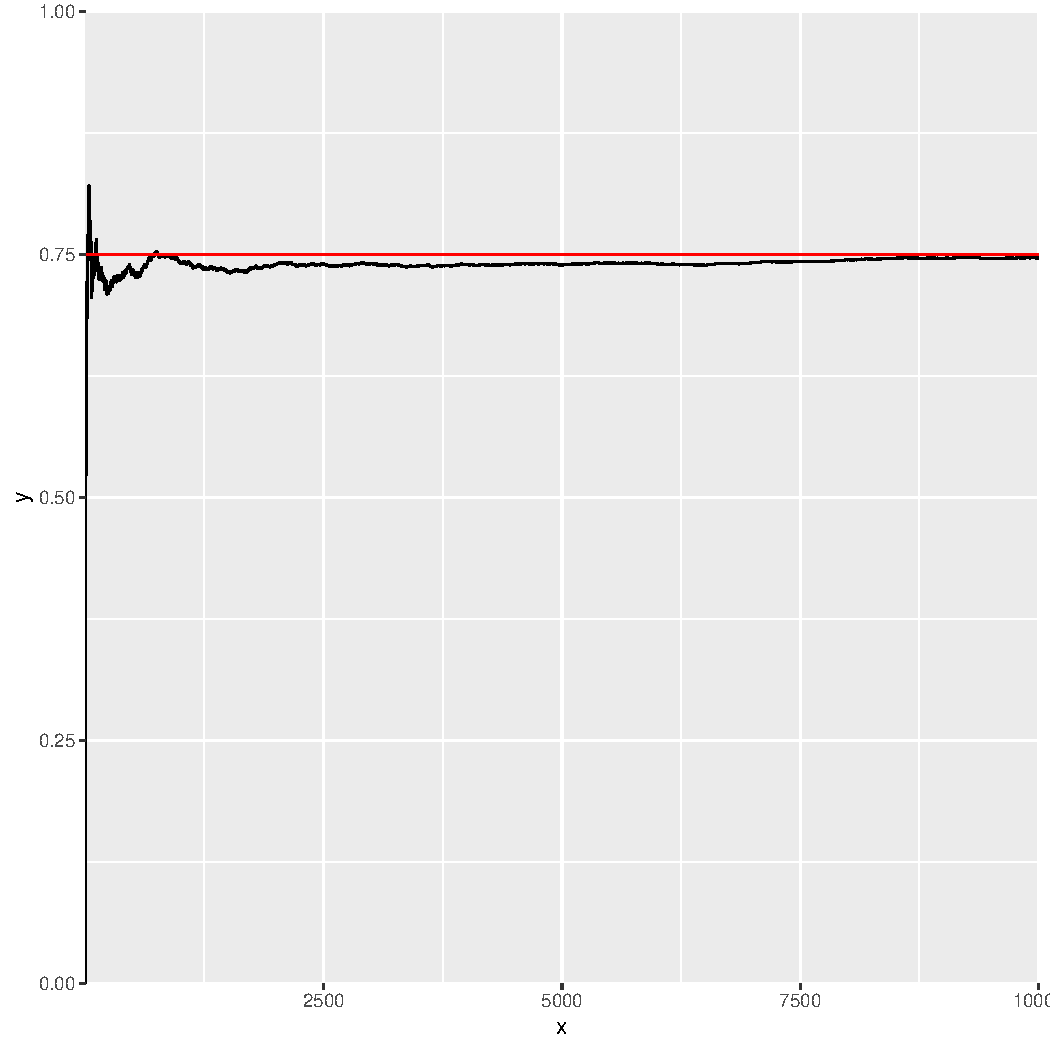
\includegraphics[width=\maxwidth]{images/statistics//unnamed-chunk-54-1} 
\end{knitrout}

\begin{knitrout}
\definecolor{shadecolor}{rgb}{0.969, 0.969, 0.969}\color{fgcolor}\begin{kframe}
\begin{alltt}
\hldef{sample_size} \hlkwb{<-} \hlnum{1000}\hlcom{#sample_size }
\hldef{k} \hlkwb{<-} \hlnum{1000}\hlcom{#number of samples}
\hldef{Many_Sample_Means_MC} \hlkwb{<-} \hlkwd{replicate}\hldef{(k,} \hlkwd{mean}\hldef{(}\hlkwd{simulate_markov_chain}\hldef{(sample_size, a, b  )))}
\hlkwd{ggplot}\hldef{(} \hlkwc{data} \hldef{=} \hlkwd{tibble}\hldef{(}\hlkwc{x} \hldef{= Many_Sample_Means_MC ))} \hlopt{+}
      \hlkwd{geom_histogram}\hldef{(} \hlkwd{aes}\hldef{( x ))} \hlopt{+}
      \hlkwd{geom_vline}\hldef{(} \hlkwc{xintercept} \hldef{= mu,} \hlkwc{col} \hldef{=} \hlsng{'red'}\hldef{)}
\end{alltt}


{\ttfamily\noindent\itshape\color{messagecolor}{\#\# `stat\_bin()` using `bins = 30`. Pick better value with `binwidth`.}}\end{kframe}
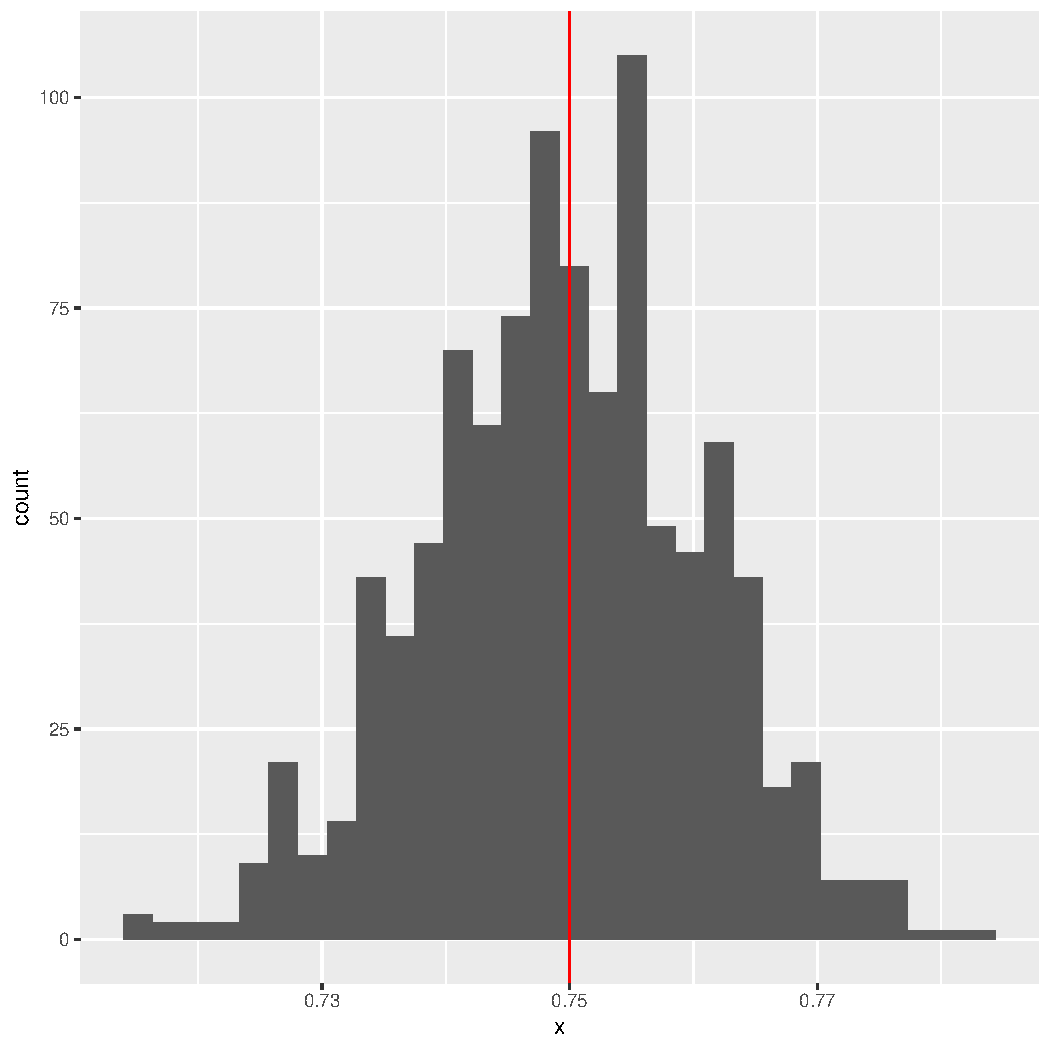
\includegraphics[width=\maxwidth]{images/statistics//unnamed-chunk-55-1} 
\end{knitrout}



The CLT for Markov Chains


\begin{knitrout}
\definecolor{shadecolor}{rgb}{0.969, 0.969, 0.969}\color{fgcolor}\begin{kframe}
\begin{alltt}
\hldef{CLT} \hlkwb{<-}\hlkwd{sqrt}\hldef{(sample_size)}\hlopt{*}\hldef{( Many_Sample_Means_MC}\hlopt{-}   \hldef{mu)}
\hlkwd{ggplot}\hldef{(} \hlkwc{data} \hldef{=} \hlkwd{tibble}\hldef{(}\hlkwc{x} \hldef{= CLT ))} \hlopt{+}
      \hlkwd{geom_histogram}\hldef{(} \hlkwd{aes}\hldef{(x,} \hlkwd{after_stat}\hldef{(density)),} \hlkwc{bins} \hldef{=} \hlnum{60}\hldef{)} \hlopt{+}
      \hlkwd{stat_function}\hldef{(} \hlkwc{fun} \hldef{=  dnorm,} \hlkwc{args} \hldef{=} \hlkwd{list}\hldef{(}\hlkwc{mean} \hldef{=} \hlnum{0}\hldef{,} \hlkwc{sd} \hldef{= sigma_Markov ),} \hlkwc{col} \hldef{=} \hlsng{'red'}\hldef{)} \hlopt{+}
      \hlkwd{stat_function}\hldef{(} \hlkwc{fun} \hldef{=  dnorm,} \hlkwc{args} \hldef{=} \hlkwd{list}\hldef{(}\hlkwc{mean} \hldef{=} \hlnum{0}\hldef{,} \hlkwc{sd} \hldef{= sigma_iid ),} \hlkwc{col} \hldef{=} \hlsng{'blue'}\hldef{)}
\end{alltt}
\end{kframe}
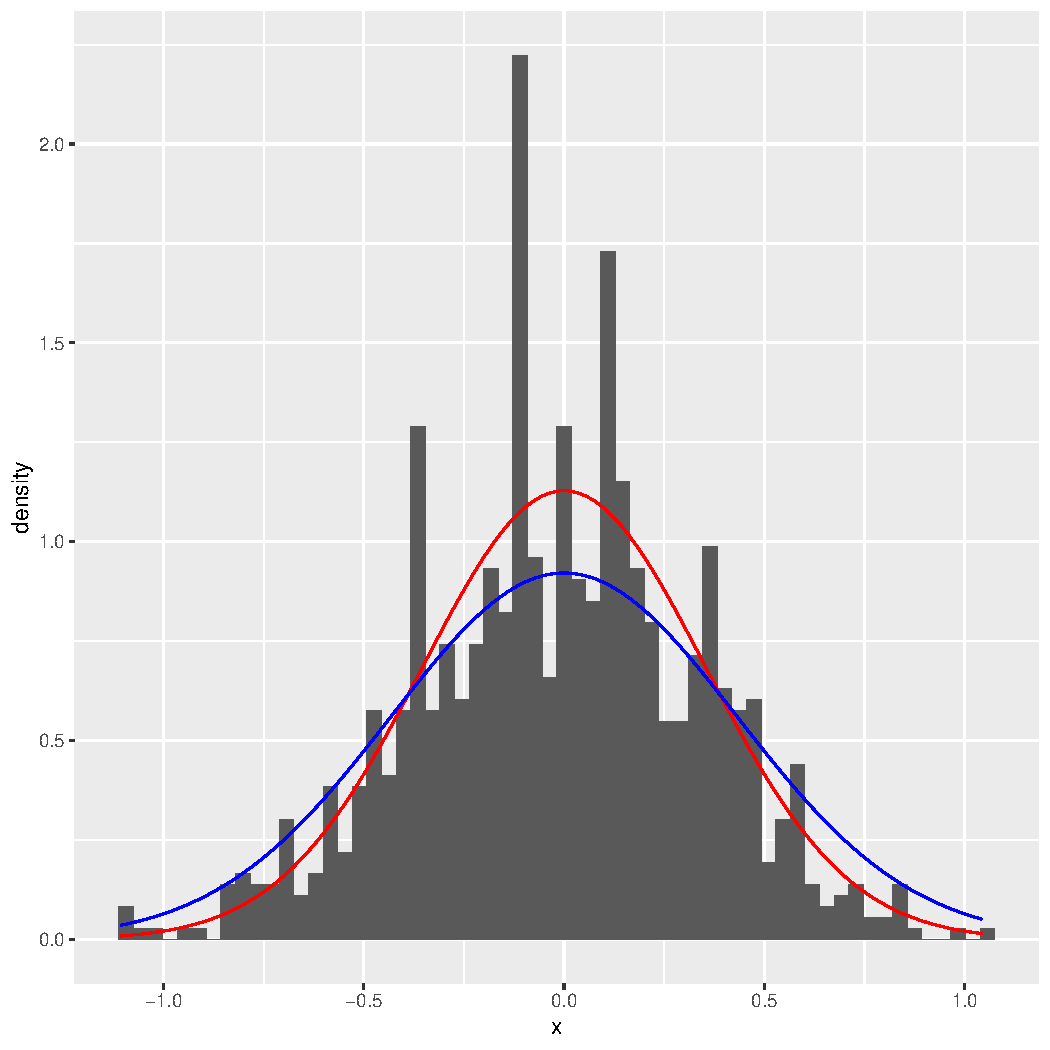
\includegraphics[width=\maxwidth]{images/statistics//unnamed-chunk-56-1} 
\end{knitrout}
\begin{knitrout}
\definecolor{shadecolor}{rgb}{0.969, 0.969, 0.969}\color{fgcolor}\begin{kframe}
\begin{alltt}
\hldef{sample_size} \hlkwb{<-} \hlnum{100000}
\hldef{MC} \hlkwb{<-} \hlkwd{simulate_markov_chain}\hldef{(sample_size, a, b)}
\hlcom{# The exponential distribution  has standard deviation 1}
\hlcom{# and mean 1}
\hldef{CLT} \hlkwb{<-} \hlkwd{sqrt}\hldef{((}\hlnum{1}\hlopt{:}\hldef{Sample_size))}\hlopt{*}\hldef{(} \hlkwd{cumsum}\hldef{(MC)}\hlopt{/}\hlnum{1}\hlopt{:}\hldef{Sample_size} \hlopt{-} \hldef{mu)}\hlopt{/}\hldef{sigma_Markov}
\hlkwd{ggplot}\hldef{(} \hlkwc{data} \hldef{=} \hlkwd{tibble}\hldef{(}\hlkwc{x} \hldef{=} \hlnum{1}\hlopt{:}\hldef{Sample_size,} \hlkwc{y} \hldef{= CLT  ))} \hlopt{+}
        \hlkwd{geom_line}\hldef{(}\hlkwd{aes}\hldef{(x,y))}
\end{alltt}
\end{kframe}
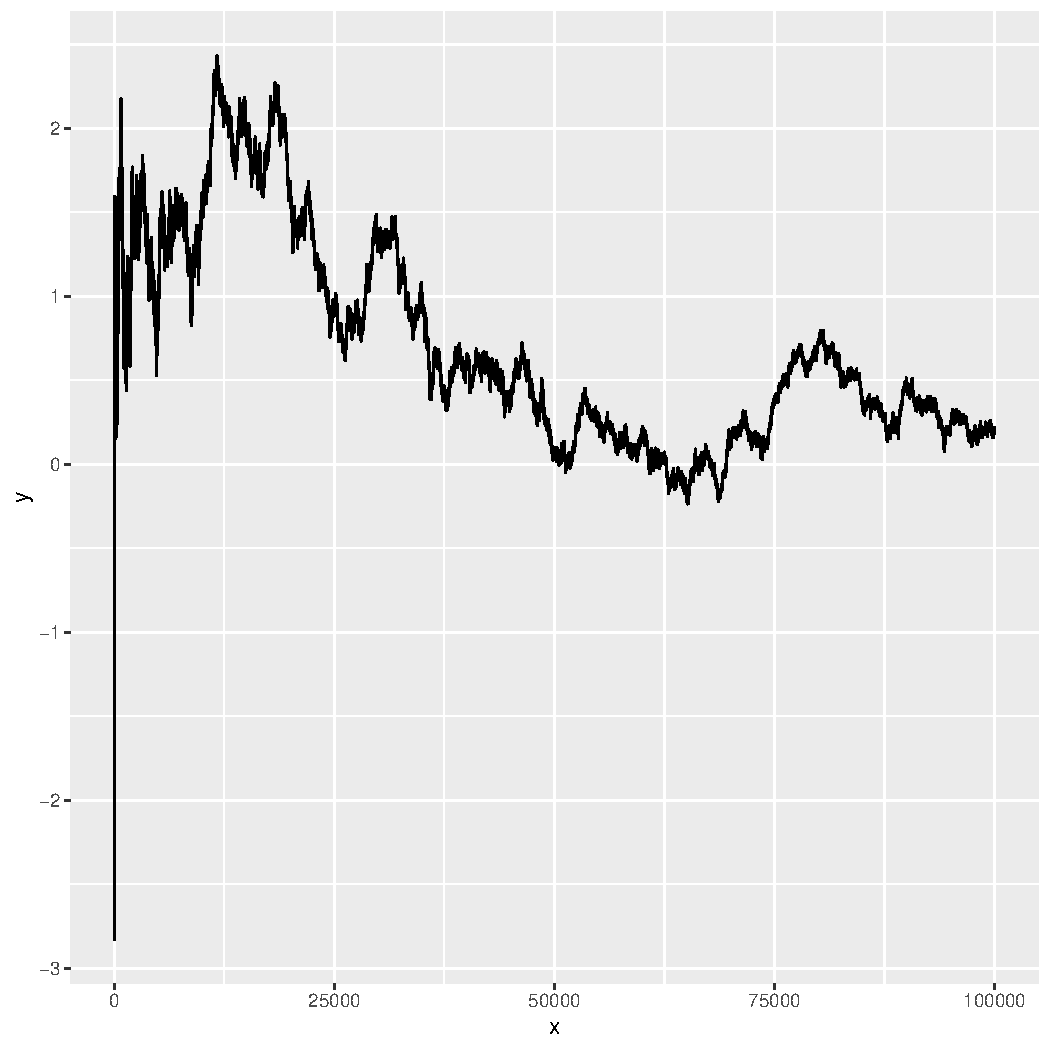
\includegraphics[width=\maxwidth]{images/statistics//unnamed-chunk-57-1} 
\end{knitrout}
	Let 
	\begin{equation}
	\label{e:Markoc}
	\left(
		\begin{array}{cc}
			1-a & a \\
			b & 1-b 
		\end{array}
	\right)
	\end{equation}
	be the transition probability of a Markov chain. This means that $a$ and $b$ are the probabilities of transitionating from $0$ to $1$ and from $1$ to $0$, respectively. We recall the model \eqref{e:Markov_model}
	\bel{}{
		& \mathbb P(X_{n+1} = 1 | X_{n} = 0 , X_{n-1} = x_{n-2}, \ldots , X_1 = x_1 ) = \mathbb P(X_{n + 1} = 1 | X_n = 0  ) = a \\ 
		& \mathbb P(X_{n+1} = 0 | X_{n} = 1 , X_{n-1} = x_{n-2}, \ldots , X_1 = x_1 ) = \mathbb P(X_{n + 1} = 1 | X_n = 0  ) = b
	}
	for each $n \in \mathbb N $ and $x_{n-1}, \ldots , x_1 \in \{0,1\}$. Given a sequence of 0s and 1s, such as the one coming from the consonants and the vowels in the Eugene Onegin
\begin{knitrout}
\definecolor{shadecolor}{rgb}{0.969, 0.969, 0.969}\color{fgcolor}\begin{kframe}
\begin{alltt}
\hlkwd{library}\hldef{(}\hlsng{'rdracor'}\hldef{)}
\hldef{ru} \hlkwb{<-} \hlkwd{get_dracor}\hldef{(}\hlkwc{corpus} \hldef{=} \hlsng{"rus"}\hldef{)}
\hldef{draa_name} \hlkwb{<-} \hldef{ru}\hlopt{$}\hldef{playName[}\hlnum{10}\hldef{]}
\hldef{text} \hlkwb{<-} \hlkwd{get_text_chr_spoken}\hldef{(}\hlkwc{play} \hldef{= drama_name,} \hlkwc{corpus} \hldef{=} \hlsng{"rus"}\hldef{)}
\end{alltt}


{\ttfamily\noindent\bfseries\color{errorcolor}{\#\# Error in stopifnot(is.character(play) \&\& length(play) == 1): oggetto 'drama\_name' non trovato}}\begin{alltt}
\hldef{all_text} \hlkwb{<-} \hlkwd{paste}\hldef{(text,} \hlkwc{collapse} \hldef{=} \hlsng{""}\hldef{)}
\end{alltt}


{\ttfamily\noindent\bfseries\color{errorcolor}{\#\# Error in paste(text, collapse = "{}"{}): cannot coerce type 'closure' to vector of type 'character'}}\begin{alltt}
\hldef{letters_vector} \hlkwb{<-} \hlkwd{unlist}\hldef{(}\hlkwd{strsplit}\hldef{(all_text,} \hlsng{""}\hldef{))}
\end{alltt}


{\ttfamily\noindent\bfseries\color{errorcolor}{\#\# Error in strsplit(all\_text, "{}"{}): oggetto 'all\_text' non trovato}}\begin{alltt}
\hldef{spoken_chars} \hlkwb{<-} \hldef{letters_vector[}\hlkwd{grepl}\hldef{(}\hlsng{"[а-яё]"}\hldef{, letters_vector)]}  \hlcom{# Keep only Russian letters}
\end{alltt}


{\ttfamily\noindent\bfseries\color{errorcolor}{\#\# Error: oggetto 'letters\_vector' non trovato}}\begin{alltt}
\hldef{russian_vowels} \hlkwb{<-} \hlkwd{strsplit}\hldef{(}\hlsng{"аеёиоуыэюя"}\hldef{,} \hlsng{""}\hldef{)[[}\hlnum{1}\hldef{]]}
\hldef{binary_sequence} \hlkwb{<-} \hlkwd{ifelse}\hldef{(spoken_chars} \hlopt \hldef{russian_vowels,} \hlnum{0}\hldef{,} \hlnum{1}\hldef{)}
\end{alltt}


{\ttfamily\noindent\bfseries\color{errorcolor}{\#\# Error in spoken\_chars \%in\% russian\_vowels: oggetto 'spoken\_chars' non trovato}}\begin{alltt}
\hldef{binary_sequence[}\hlnum{1}\hlopt{:}\hlnum{10}\hldef{]}
\end{alltt}


{\ttfamily\noindent\bfseries\color{errorcolor}{\#\# Error: oggetto 'binary\_sequence' non trovato}}\end{kframe}
\end{knitrout}


	an estimate for the parametes $a$ and $b$ is given by the functional of the flux (not of the current)  
	\bel{}{
		\bar b = \frac{1}{n} \sum_{i = 1}^{n-1} \chi(X_i = 0,  X_{i + 1} =1)  
		\bar a = \frac1n \sum_{i = 1 }^{n-1}\chi(X_i = 1, X_{i + 1} = 0)
	}
	This is for me: The invariant measure of the dynamics depends on the ratio between the transitions from 0 to 1 (b) and from 1 to 0 (a) (the current )
	$\pi_0 b = \pi_1 a $, so that $(\pi_0, \pi_1 )  = (a,b )/(a+b)$. In particular, we have two estimates for $p = \pi_1$: the is given by $\bar b / \bar a + \bar b$, and the standard empirical one. 
	\section{Central limit theorem for the Markov Sequence }	


	\bel{}{
		\bar b = \frac{1}{n} \sum_{i = 1}^{n-1} \chi(X_i = 0,  X_{i + 1} =1)  
		\bar a = \frac1n \sum_{i = 1 }^{n-1}\chi(X_i = 1, X_{i + 1} = 0)
	}
	\begin{equation}
	\label{e:Markoc}
	\left(
		\begin{array}
			1-a & a \\
			b & 1-b 
		\end{array}
	\right)
	\end{equation}
	Let's compute the variance of $\sum_{ i = 1 \ldots }\frac1{\sqrt{n}} \left( X_i - \pi_i \right)$. This is given by 
	\bel{}{
		\frac1n	\sum_{i, j} E\left[ (X_i - \pi_i)(X_j -\pi_j)\right]
	}	
	and, assuming we start from the invariant measure, it becomes 
	\bel{}{
	\text{Var}_\pi(X_0) + \sum_{i =1}^{+\infty}\text{Cov}_\pi(X_i , X_0 )) = \sigma
	}
	We need to compute the mean of $ P^n_{i,j}f_if_j$. Since the covariace function that we want to compute is already mean zero, meaning that $f = (-\pi_1, 1- \pi_1 )$ has mean with respec to to $\pi$ given $- \pi_0\pi_1 + \pi_1 - \pi_1^2 = \pi_1(1 - \pi_1 - \pi_2) = 0 $ since $\pi$ is a probability measure. Indeed $f = (-\pi_1  ,\pi_0)$ Indeed $(-\pi_1, \pi_0)$ and the harmonic $(1,1)$ function $\pi$ ar ean orthonormal basis in $L^2(\pi)$. Therefoe 
	\bel{}{
		\text{Cov}_\pi(X_0, X_n ) = \lambda_2^n < (\cdot - \pi_1 ),(\cdot - \pi_1) >_\pi = \lambda_2^n \text{Var}_\pi(X_0)  
	} 
	This gives us 
	that the varaince of the variable in the central limit theorem is 
	\bel{}{
		\text{Var}_\pi(X_0)\frac{1}{1- \lambda_2}
	}
	where $\lambda_2$ is the second eigenvalue (it is in general like that? no there are the smaller effects of the other eigenvalues ) 
	The variance of $X_0$ is $ \pi_0\pi^2_1 + \pi_1(1 - \pi_1)^2  = \pi_1^2  + \pi_1 - 2\pi_1^2  = \pi_1( 1- \pi_1)$ (of course, si a Bernoulli) and $\lambda_2 = 1- a - b$, so that 
	\bel{}{
		\sigma^2 = \frac{ b/(a + b) a/(a + b)}{ a + b } = \frac{ab}{(a + b)^2} 
	}
	which is the sigma for our variable 
	\section{ Eugene Onegin }
		\subsection{Eugene Onegin}
		We now see that the Markov model 
		We come backk to Example~\ref{ex:Eugene_Onegin1} and place it in the statisitical setting introduced in Subsection~\ref{ss:model} and Section~\ref{s:testing}. Recall that from the texts of the german drama corpus we have defined a sequence $\underline X = X_1 X_2 \ldots X_N$ of $N$ digits $X_i$ that are either $1$, if the $i$-th character is a consonant of 0 if it is a vowel, neglecting all the other characters and empty spaces. \\
	The first model $H_0$ says that $H_0$ is obtained from the distribution by 
